%%%%%%%%%%%%%%%%%%%%%%%%%%%%%%%%%%%%%%%%%%%%%%%%%%%%%%%%%%%%%%%%%%%%
\section{Design}
\label{sec:fdsp-apa-design}

The physics performance of the \dword{spmod} is a function of many intertwined detector parameters including argon purity, drift distance, \efield, wire pitch, wire length, and noise levels in the readout \dword{ce}.  Energy deposits from \dwords{mip} originating anywhere inside the active volume of the detector should be identifiable with near \num{100}\% efficiency.  This requirement constrains aspects of the \dword{apa} design, specifically, the limits on wire pitch, wire length, and choice of wire material.  This section details the design of an individual \dword{apa}. We begin with an overview of the key fundamental parameters of the \dwords{apa} and their connection to the physics requirements of the experiment. 


%%%%%%%%%%%%%%%%%%%%%%%%%%%%%%%%%%%%%%%%%%%%%%%%%%%%%%%%%%%%%%%%%%%%
\subsection{APA Design Parameters}
\label{sec:fdsp-apa-design-overview}

Each \dword{apa} is \SI{6}{m} high, \SI{2.3}{m} wide, and \SI{15}{cm} thick.  The underlying support frame is made from stainless steel hollow tube sections that are precisely machined and bolted together. A fine, conducting mesh covers the rectangular openings in the frame on both sides, to define a uniform electrical \dword{gp} behind the wires. The four layers of sense and shielding wires at varying angles relative to each other completely cover the frame. The wires terminate on boards that anchor them as well as providing the connection to the \dword{tpc} readout \dword{ce}. Starting from the outermost wire layer, there is first an uninstrumented shielding plane (vertical, $G$), followed by two induction planes (\apainducwireangle to the vertical, $U,V$), and finally the collection plane (vertical, $X$). All wire layers span the entire height of the \dword{apa} frame. The two planes of induction wires wrap in a helical fashion around the long edges and over both sides of the \dword{apa}. Figures~\ref{fig:tpc_apa1} and \ref{fig:tpc_apa2} illustrate the layout of the wire layers.  Below, we summarize the key design parameters and the considerations driving the main design choices for the \dwords{apa}.  A tabulated summary of \dword{apa} specific requirements are also provided in Table~\ref{tab:SP-APA-specs}. %Appendix \ref{ch:sp-reqs}.   %A complete list of \dword{apa} design requirements can be found in DUNE-docdb-6416. 

%\fixme{Anne added new tables here 12/10. Updated 12/14 (generated longtable)}

% This file is generated, any edits may be lost.

% It defines macros which expand to corresponding
% specification values for subsystem SP-APA



\begin{longtable}{p{0.14\textwidth}p{0.13\textwidth}p{0.18\textwidth}p{0.22\textwidth}p{0.20\textwidth}}
\caption{Specifications for SP-APA \fixmehl{ref \texttt{tab:spec:SP-APA}}} \\
  \rowcolor{dunesky}
       Label & Description  & Specification \newline (Goal) & Rationale & Validation \\  \colhline

   \newtag{SP-FD-1}{ spec:min-drift-field }  & Minimum drift field  &  $>$\,\SI{250}{ V/cm} \newline ( $>\,\SI{500}{ V/cm}$ ) &  Lessens impacts of $e^-$-Ar recombination, $e^-$ lifetime, $e^-$ diffusion and space charge. &  ProtoDUNE \\ \colhline
    
   
  \newtag{SP-FD-2}{ spec:system-noise }  & System noise  &  $<\,\SI{1000}\,e^-$ &  Provides $>$5:1 S/N on induction planes for  pattern recognition and two-track separation. &  ProtoDUNE and simulation \\ \colhline
    
   
  \newtag{SP-FD-3}{ spec:light-yield }  & Light yield  &  $>\,\SI{20}{PE/MeV}$ (avg), $>\,\SI{0.5}{PE/MeV}$ (min) &  Gives PDS energy resolution comparable that of the TPC for 5-7 MeV SN $\nu$s, and allows tagging of $>\,\SI{99}{\%}$ of nucleon decay backgrounds with light at all points in detector. &  Supernova and nucleon decay events in the FD with full simulation and reconstruction. \\ \colhline
    
    \\ \rowcolor{dunesky} \newtag{SP-FD-4}{ spec:time-resolution-pds } & Name: Time resolution \\
    Description & The time resolution of the photon detection system shall be less than 1 microsecond in order to assign a unique event time.   \\  \colhline
    Specification (Goal) &  $<\,\SI{1}{\micro\second}$  ( $<\,\SI{100}{\nano\second}$ ) \\   \colhline
    Rationale &   Enables \SI{1}{mm} position resolution for \SI{10}{MeV} SNB candidate events for instantaneous rate $<\,\SI{1}{m^{-3}ms^{-1}}$.  \\ \colhline
    Validation &   \\
   \colhline

   \newtag{SP-FD-5}{ spec:lar-purity }  & Liquid argon purity  &  $<$\,\SI{100}{ppt} \newline ($<\,\SI{30}{ppt}$) &  Provides $>$5:1 S/N on induction planes for  pattern recognition and two-track separation. &  Purity monitors and cosmic ray tracks \\ \colhline
    
    \\ \rowcolor{dunesky} \newtag{SP-FD-6}{ spec:apa-gaps } & Name: Gaps between APAs  \\
    Description & The gap size between APAs shall minimize loss of fiducial volume and distortion of charge collection.   \\  \colhline
    Specification &  $<\,\SI{15}{mm}$ between APAs on same support beam; $<\,\SI{30}{mm}$ between APAs on different support beams \\   \colhline
    Rationale &   Maintains fiducial volume.  Simplified contruction.  \\ \colhline
    Validation & ProtoDUNE  \\
   \colhline

    \\ \rowcolor{dunesky} \newtag{SP-FD-7}{ spec:misalignment-field-uniformity } & Name: Drift field uniformity due to component alignment \\
    Description & Misalignments of the various TPC components shall not introduce drift-field nonuniformities beyond those specified in the HVS requirements.   \\  \colhline
    Specification &  $<\,1\,$\% throughout volume \\   \colhline
    Rationale &   Maintains APA, CPA,  FC orientation and shape.  \\ \colhline
    Validation & ProtoDUNE  \\
   \colhline

    
   
  \newtag{SP-FD-8}{ spec:apa-wire-angles }  & APA wire angles  &  \SI{0}{\degree} for collection wires, \SI{35.7}{\degree} for induction wires &  Minimize inter-APA dead space. &  Engineering calculation \\ \colhline
    
    
   
  \newtag{SP-FD-9}{ spec:apa-wire-spacing }  & APA wire spacing  &  \SI{4.669}{mm} for U,V; \SI{4.790}{mm} for X,G &  Enables 100\% efficient MIP detection, \SI{1.5}{cm} $yz$ vertex resolution. &  Simulation \\ \colhline
    
   
  \newtag{SP-FD-10}{ spec:apa-wire-pos-tolerance }  & APA wire position tolerance  &  $\pm\,\SI{0.5}{mm}$ &  Interplane electron transparency; $dE/dx$, range, and MCS calibration. &  ProtoDUNE and simulation \\ \colhline
    

    \\ \rowcolor{dunesky} \newtag{SP-APA-1}{ spec:apa-unit-size } & Name: APA unit size \\
    Description & Overall dimensions of a single anode plane assembly   \\  \colhline
    Specification &  \SI{6.0}{m} tall $\times$ \SI{2.3}{m} wide \\   \colhline
    Rationale &   Maximum size allowed for fabrication, transportation, and installation.   \\ \colhline
    Validation & ProtoDUNE-SP   \\
   \colhline

   
  \newtag{SP-APA-2}{ spec:apa-active-area }  & Active area  &  Maximize total active area. &  Maximize area for data collection  &  ProtoDUNE-SP  \\ \colhline
    
   
  \newtag{SP-APA-3}{ spec:apa-wire-tension }  & Wire tension  &  \SI{6}{N} $\pm$ \SI{1}{N} &  Prevent contact beween wires and minimize  break risk &  ProtoDUNE-SP \\ \colhline
    
    \\ \rowcolor{dunesky} \newtag{SP-APA-4}{ spec:apa-bias-voltage } & Name: Wire plane bias voltages \\
    Description & APAs should produce optimal and uniform induction and collection signal shapes.   \\  \colhline
    Specification &  The setup, including boards, must hold 150\% of max operating voltage. \\   \colhline
    Rationale &   Headroom in case adjustments needed  \\ \colhline
    Validation & E-field simulation sets wire bias voltages. ProtoDUNE-SP confirms performance.  \\
   \colhline

    
   
  \newtag{SP-APA-5}{ spec:apa-frame-planarity }  & Frame planarity (twist limit)  &  $<$\SI{5}{mm} &  APA transparency.  Ensures wire plane spacing change of $<$0.5 mm.  &  ProtoDUNE-SP \\ \colhline
    
    
   
  \newtag{SP-APA-6}{ spec:apa-bad-channels }  & Missing/unreadable channels  &  $<$1\%, with a goal of $<$0.5\% &  Reconstruction efficiency &  ProtoDUNE-SP \\ \colhline
    


\label{tab:specs:SP-APA}
\end{longtable}
%% This file is generated, any edits may be lost.

% It defines macros which expand to corresponding
% specification values for subsystem SP-APA



\begin{longtable}{p{0.13\textwidth}p{0.15\textwidth}p{0.22\textwidth}p{0.25\textwidth}p{0.18\textwidth}}    

\caption{Specifications for SP-APA \fixmehl{ref \texttt{tab:specs:SP-APA}}} \\

\rowcolor{dunesky}
  Label & Name  & Specification \newline (Goal) & Rationale & Validation \\  \colhline

  \newtag{SP-FD-1}{ spec:min-drift-field }  & Minimum drift field  &  $>$\,\SI{250}{ V/cm} \newline ( $>\,\SI{500}{ V/cm}$ ) &  Lessens impacts of e-Ar recombination, e-lifetime, e-diffusion and space charge. &  ProtoDUNE \\ \colhline
    
 
 \newtag{SP-FD-2}{ spec:system-noise }  & System noise  &  $<\,\SI{1000}{enc}$ &  Provides $>$5:1 S/N on induction planes for  pattern recognition and two-track separation. &  ProtoDUNE and simulation \\ \colhline
 
   \newtag{SP-FD-3}{ spec:light-yield }  & Light yield  &  $>\,\SI{0.5}{pe/MeV}$ \newline ( $>\,\SI{5}{pe/MeV}$ ) &  Rejects nucleon decay backgrounds from cosmogenic events near cathode. &   \\ \colhline
  
 \newtag{SP-FD-4}{ spec:time-resolution-pds }  & Time resolution  &  $<\,\SI{1}{\micro\second}$ \newline ( $<\,\SI{100}{\nano\second}$ ) &  Enables \SI{1}{mm} position resolution for \SI{10}{MeV} SNB candidate events for instantaneous rate $<\,\SI{1}{m^{-3}ms^{-1}}$. &   \\ \colhline
 
 
   \newtag{SP-FD-5}{ spec:lar-purity }  & Liquid argon purity  &  $<$\,\SI{100}{ppt} \newline ( $<\,\SI{30}{ppt}$ ) &  Provides $>$5:1 S/N on induction planes for  pattern recognition and two-track separation. &  Purity monitors and cosmic ray tracks \\ \colhline
    

 \newtag{SP-FD-6}{ spec:apa-gaps }  & Gaps between APAs   &  $<\,\SI{15}{mm}$ between APAs on same support beam; $<\,\SI{30}{mm}$ between APAs on different support beams &  Maintains fiducial volume.  Simplified contruction. &  ProtoDUNE \\ \colhline

 \newtag{SP-FD-7}{ spec:misalignment-field-uniformity }  & Drift field uniformity due to component alignment  &  $<\,1\,$\% throughout volume &  Maintains APA, CPA,  FC orientation and shape. &  ProtoDUNE \\ \colhline
   
  \newtag{SP-FD-8}{ spec:apa-wire-angles }  & APA wire angles  &  \SI{0}{\degree} for collection wires, \SI{35.7}{\degree} for induction wires &  Minimize inter-APA dead space. &  Engineering calculation \\ \colhline
   
   \newtag{SP-FD-9}{ spec:apa-wire-spacing }  & APA wire spacing  &  \SI{4.669}{mm} for U,V; \SI{4.790}{mm} for X,G &  Enables 100\% efficient MIP detection, \SI{1.5}{cm} $yz$ vertex resolution. &  Simulation \\ \colhline
   
   \newtag{SP-FD-10}{ spec:apa-wire-pos-tolerance }  & APA wire position tolerance  &  $\pm\,\SI{0.5}{mm}$ &  Interplane electron transparency; $dE/dx$, range, and MCS calibration. &  ProtoDUNE and simulation \\ \colhline
    
 % \newtag{SP-APA-1}{ spec:apa-unit-size }  & Overall dimensions of a single anode plane assembly  &  \SI{6.0}{m} tall $\times$ \SI{2.3}{m} wide &  Maximum size allowed for fabrication, transportation, and installation.  &  ProtoDUNE-SP  \\ \colhline
    \newtag{SP-APA-1}{ spec:apa-unit-size }  & APA unit size  &  \SI{6.0}{m} tall $\times$ \SI{2.3}{m} wide &  Maximum size allowed for fabrication, transportation, and installation.  &  ProtoDUNE-SP  \\ \colhline 
    

%  \newtag{SP-APA-2}{ spec:apa-active-area }  & APAs should be sensitive over most of the full area of an APA frame, limiting dead regions in the detector volume.  &  Maximize total active area. &  Maximize area for data collection  &  ProtoDUNE-SP  \\ \colhline
 \newtag{SP-APA-2}{ spec:apa-active-area }  & Active area  &  Maximize total active area. &  Maximize area for data collection  &  ProtoDUNE-SP  \\ \colhline
    
    

 % \newtag{SP-APA-3}{ spec:apa-wire-tension }  & APA wires shall not touch during operation and break risk must be kept to a minimum.   &  \SI{6}{N} $\pm$ \SI{1}{N} &  Prevent contact beween wires and minimize  break risk &  ProtoDUNE-SP \\ \colhline
     \newtag{SP-APA-1}{ spec:apa-unit-size }  & APA unit size  &  \SI{6.0}{m} tall $\times$ \SI{2.3}{m} wide &  Maximum size allowed for fabrication, transportation, and installation.  &  ProtoDUNE-SP  \\ \colhline

%  \newtag{SP-APA-4}{ spec:apa-bias-voltage }  & APAs should produce optimal and uniform induction and collection signal shapes.  &  The setup, including boards, must hold 150\% of max operating voltage. &  Headroom in case adjustments needed &  E-field simulation sets wire bias voltages. ProtoDUNE-SP confirms performance. \\ \colhline
 \newtag{SP-APA-4}{ spec:apa-bias-voltage }  & Wire plane bias voltages  &  The setup, including boards, must hold 150\% of max operating voltage. &  Headroom in case adjustments needed &  E field simulation sets wire bias voltages. ProtoDUNE-SP confirms performance. \\ \colhline    
    

%  \newtag{SP-APA-5}{ spec:apa-frame-planarity }  & Overall twist of the APA frame.  &  $<$\SI{5}{mm} &  APA transparency.  Ensures wire plane spacing change of $<$0.5 mm.  &  ProtoDUNE-SP \\ \colhline
  \newtag{SP-APA-5}{ spec:apa-frame-planarity }  & Frame planarity (twist limit)  &  $<$\SI{5}{mm} &  APA transparency.  Ensures wire plane spacing change of $<$0.5 mm.  &  ProtoDUNE-SP \\ \colhline  
    

%  \newtag{SP-APA-6}{ spec:apa-bad-channels }  & Number of channels incapable of recording signals.  &  $<$1\%, with a goal of $<$0.5\% &  Reconstruction efficiency &  ProtoDUNE-SP \\ \colhline
     \newtag{SP-APA-6}{ spec:apa-bad-channels }  & Missing/ unreadable channels  &  $<$1\%, with a goal of $<$0.5\% &  Reconstruction efficiency &  ProtoDUNE-SP \\ \colhline
    
\label{tab:SP-APA-specs}

\end{longtable}  %need to replace; anne 1/8

\begin{itemize}
\item \textbf{\dword{apa} size.} The size of the \dwords{apa} is chosen for fabrication purposes, compatibility with over-the-road shipping, and for eventual transport to the \SI{4,850}{ft}~level at \dword{surf} and installation into the membrane cryostat of a \dword{detmodule}. The dimensions are also chosen so that an integral number of electronic readout channels and boards fill in the full area of the \dword{apa}.

%\fixme{Nora: anode plane assemblies in first sentence of following section should be capitalized (Anode).}

\item \textbf{Detector active area} \dword{apa}s should be sensitive over most of the full area of an \dword{apa} frame, with dead regions between \dwords{apa} due to frame elements, wire boards, electronics, or cabling kept to a minimum.  The wrapped style shown in Figure~\ref{fig:tpc_apa1} allows all channels to be read out at the top of the \dword{apa}, eliminating the dead space between \dwords{apa} that would otherwise be created by electronics and associated cabling. In addition, in the design of the \dword{spmod}, a central row of \dwords{apa} is flanked by drift-field regions on either side (see Figure~\ref{fig:FarDet-interior}), and the wrapped design allows the induction plane wires to sense drifted ionization that originates from either side of the \dword{apa}.  This double-sided feature is also effective for the \dwords{apa} located against the cryostat walls where the drift field is on only one side; the grid layer facing the wall effectively blocks any ionization generated outside the \dword{tpc} from drifting in to the wires on that side of the \dword{apa}.        

\item \textbf{Wire angles} The $X$ wires run vertically to provide optimal reconstruction of beam-induced particle tracks, which are predominantly forward (in the beam direction). The angle of the induction planes on the \dword{apa}, \apainducwireangle, was chosen to ensure that each induction wire only crosses a given collection wire once, reducing the ambiguities that the reconstruction must address.  Simulation studies (see next item) show that this configuration performs similarly to an optimal 45$^\circ$ wire angle for the primary \dword{dune} physics channels.  The design angle of the induction wires, coupled with their pitch, was also chosen so an integer multiple of electronics boards is needed to read out one \dword{apa}.

\item \textbf{Wire pitch} The choice of wire pitch, \xgpitch for $(X,G)$ and \uvpitch for $(U,V)$, combined with key parameters for other \dword{tpc} systems (described in their respective sections of the \dword{tdr}), can achieve the required performance for energy deposits by \dwords{mip} while providing good tracking resolution and good granularity for particle identification. The \single requirement that it be possible to determine the fiducial volume to \num{1}\% implies a vertex resolution of \SI{1.5}{cm} along each coordinate direction. The $\sim$\uvpitch %\SI{4.7}{mm}
\fixme{check - uvpitch?} wire pitch achieves this for the $y$ and $z$ coordinates.  The resolution on $x$, the drift coordinate, will be better than in the $y$--$z$ plane because of the combination of drift velocity and electronics sampling rate.  Finally, as already mentioned, the total number of wires on an \dword{apa} should match the granularity of the electronics boards (each \dword{femb} can read out \num{128} wires, mixed between the $U,V,X$ planes). This determines the exact wire spacings of \xgpitch on the collection plane and \uvpitch on the induction planes.  To achieve the reconstruction precision required (e.g., for $dE/dx$ reconstruction accuracy and multiple Coulomb scattering determination), the tolerance on the wire pitch is \wirepitchtol.

In 2017, the \dword{dune} \dword{fd} task force, using a full \dword{fd} simulation and reconstruction chain, performed many detector optimization studies to quantify the impact of design choices, including wire pitch and wire angle, on \dword{dune} physics performance.  The results indicated that reducing wire spacing (to \SI{3}{mm}) or changing wire angle (to \num{45}$^\circ$) would not significantly affect the performance for the main physics goals of \dword{dune}, including $\nu_\mu $ to $\nu_e$ oscillations and \dword{cpv} sensitivity.  Figure~\ref{fig:e-gamma} reproduces two plots from the task force report showing the effect of wire pitch and orientation on distinguishing electrons versus photons in the detector.  This is a key low-level metric for oscillation physics because photon induced showers can fake electron showers and create neutral-current generated backgrounds in the $\nu_e$ \dword{cc} event sample. Two important handles for reducing this contamination are the energy density at the start of the shower and the visible gap between a photon shower and the vertex of the neutrino interaction due to the non-zero photon interaction length.  Figure~\ref{fig:e-gamma}(a) shows the reconstructed ionization energy loss density ($dE/dx$) in the first centimeters of electron and photon showers, illustrating the separation between the single \dword{mip} signal from electrons and the double \dword{mip} signal when photons pair-produce an $e^+e^-$.  The final electron signal selection efficiency is shown as a function of the background rejection rate for different wire configurations in Figure~\ref{fig:e-gamma}(b). At a signal efficiency of \num{90}\,\%, for example, the background rejection can be improved by about \num{1}\,\% using either \SI{3}{mm} spacing or 45$^\circ$ wire angles for the induction planes.  This slight improvement in background rejection with more dense hit information or more optimal wire angles is not surprising, but the effect on high-level physics sensitivities from these changes is very small. The conclusions of the \dword{fd} task force, therefore, were that the introduction of ambiguities into the reconstruction by increasing the wire angles is not a good trade off, and the increase in cost incurred by decreasing the wire pitch (and, therefore, increasing the number of readout channels) is not justified.  

\begin{dunefigure}[Electron-photon separation dependence on wire pitch and angle]{fig:e-gamma}
{Summary of electron--photon separation performance studies from the \dword{dune} \dword{fd} task force. (a) $e$--$\gamma$ separation by $dE/dx$ for the nominal wire spacing and angle (\SI{4.7}{mm}/$37.5^\circ$) compared to \SI{3}{mm} spacing or 45$^\circ$ induction wire angles. (b) Electron signal selection efficiency versus photon (background) rejection for the different detector configurations. The \SI{3}{mm} wire pitch and 45$^\circ$ wire angle have similar effects, so the 45$^\circ$ curve is partly obscured by the \SI{3}{mm} curve.}
(a)
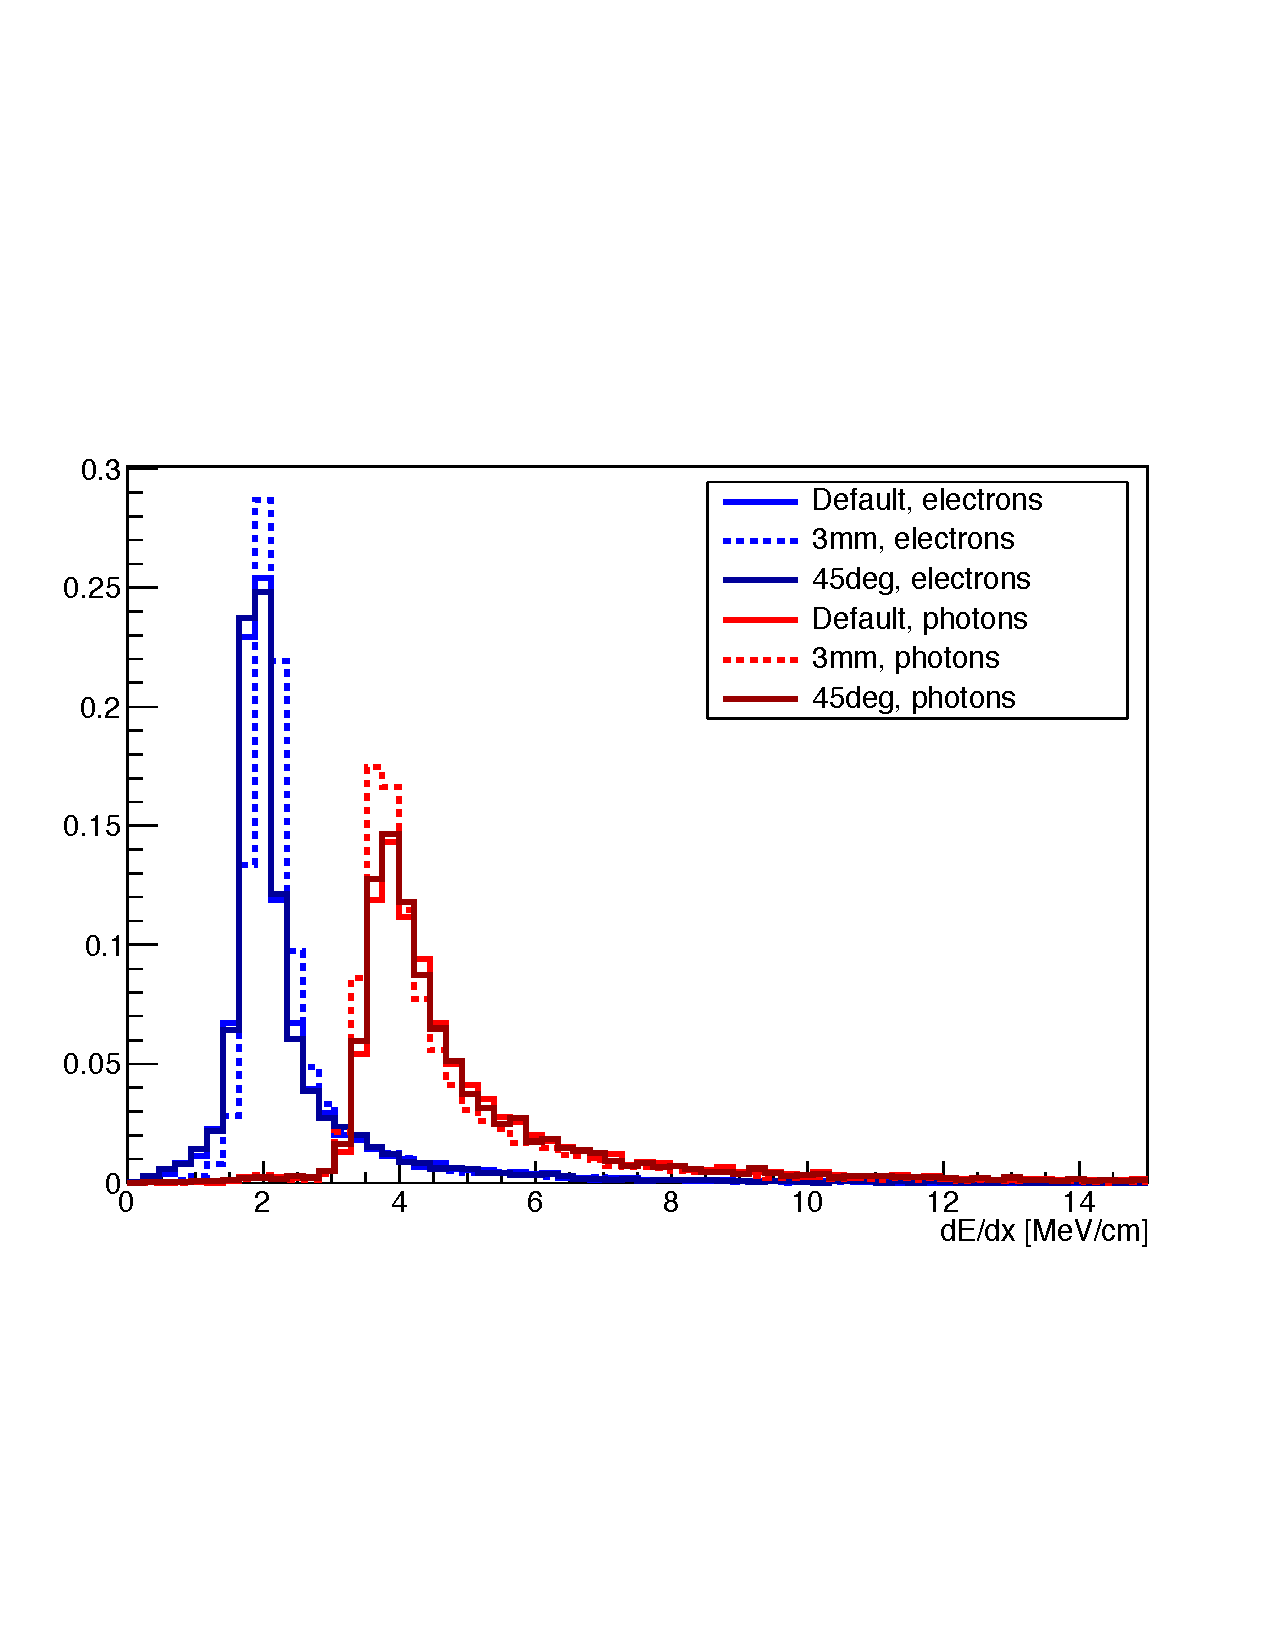
\includegraphics[height=0.24\textheight]{sp-apa-e-gamma-dEdx.pdf} \qquad
(b)
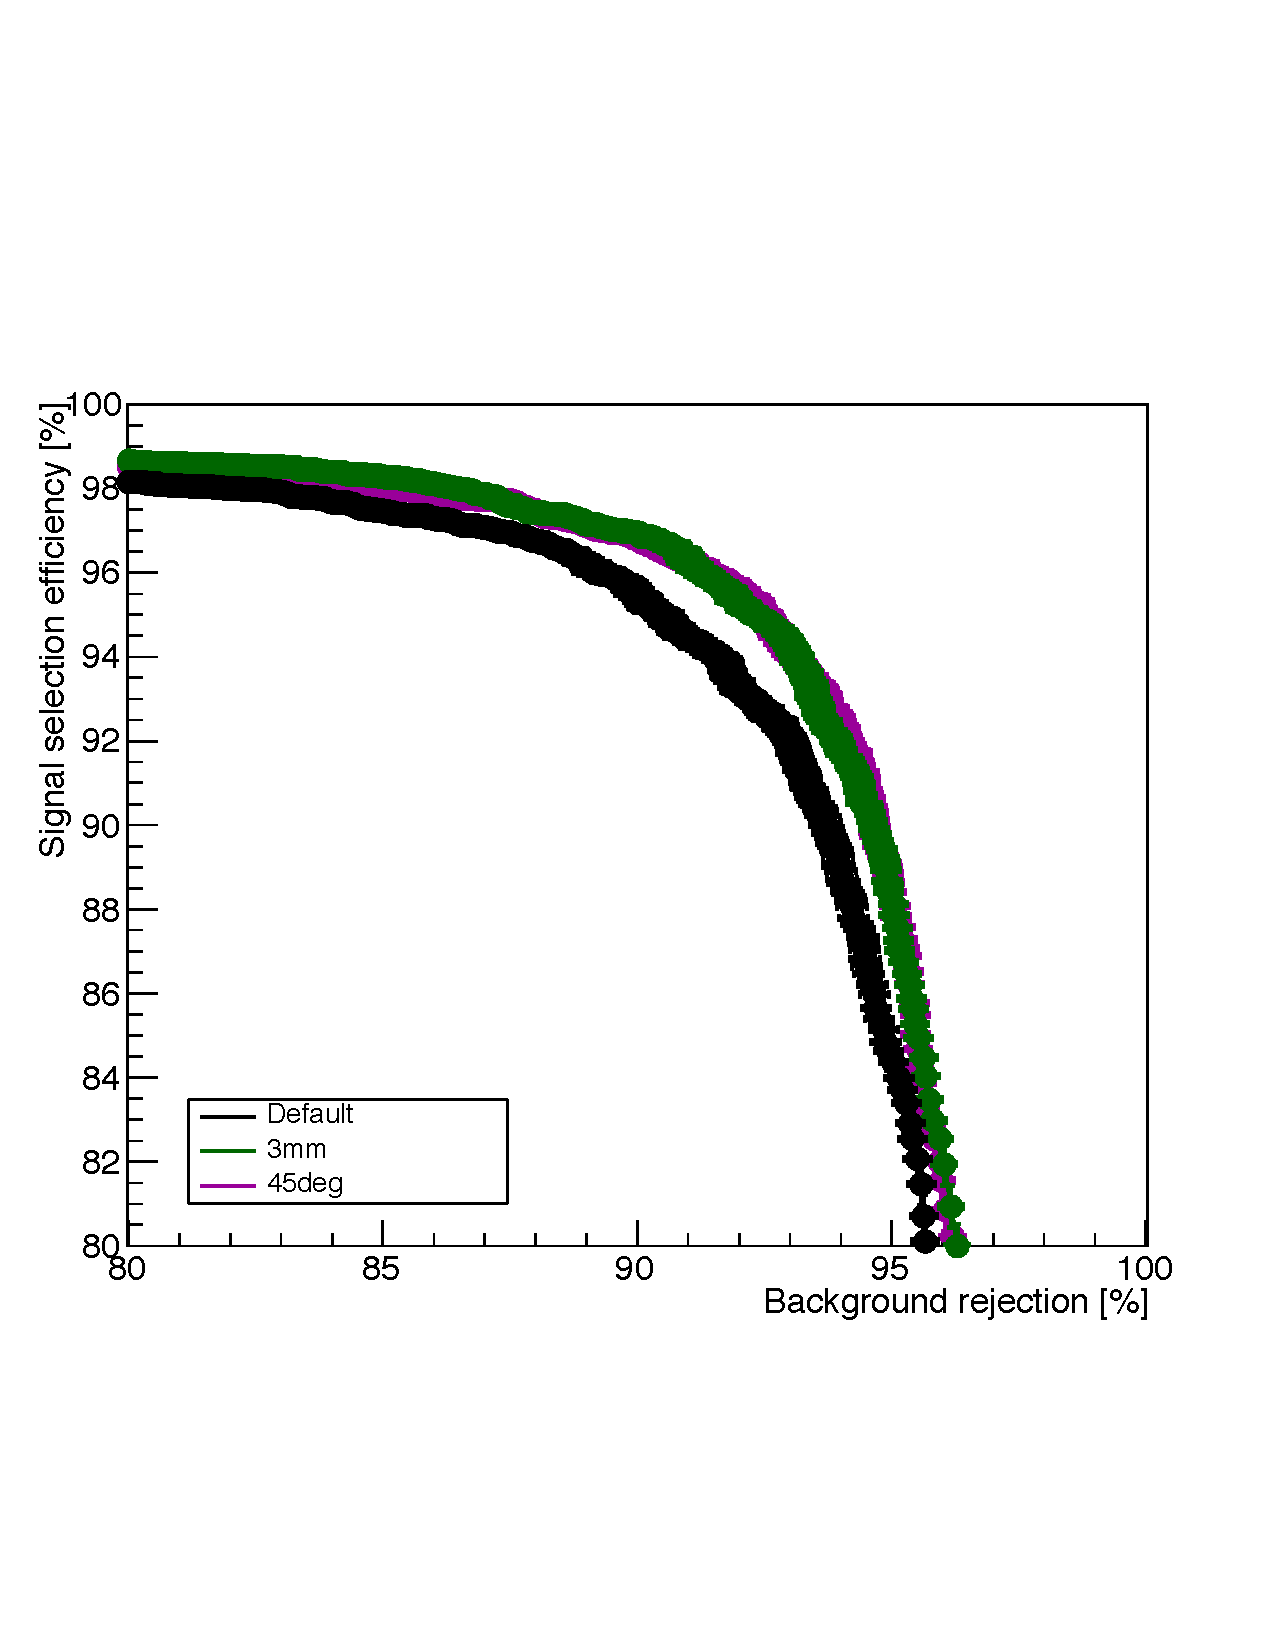
\includegraphics[height=0.24\textheight]{sp-apa-eff-bkgd-wires.pdf} 
\end{dunefigure}

\item \textbf{Wire plane transparency and signal shapes.}  The ordering of the layers, from the outside in, is $G$-$U$-$V$-$X$, followed by the grounding mesh. The operating voltages of the \dword{apa} layers are listed in Table~\ref{tab:bias}.  Figure~\ref{fig:apa-fields} shows the field simulation and expected signal shapes for the bias voltages listed in the table.  When operated at these voltages, the drifting ionization follows trajectories around the grid and induction wires, terminating on a collection plane wire. The grid and induction layers are completely transparent to drifting ionization, and the collection plane is completely opaque.  The grid layer is present for pulse-shaping and not connected to the electronics readout; it effectively shields the first induction plane from the drifting charge and removes the long leading edge from the signals on that layer. 


\begin{table}[ht]
\begin{minipage}[b]{0.46\linewidth}
\centering
\begin{tabular}{ l  r }
    \hline
   \rowcolor{dunesky} \textbf{Anode Plane} & \textbf{Bias Voltage} \\ \toprowrule
	$G$ - Grid & \SI{-665}{V} \\ \colhline
	$U$ - Induction & \SI{-370}{V{}} \\ \colhline
	$V$ - Induction & \SI{0}{V} \\ \colhline
	$X$ - Collection & \SI{820}{V} \\ \colhline
	Grounding Mesh & \SI{0}{V} \\ \colhline
    \end{tabular}
    \caption{Baseline bias voltages for \dword{apa} wire layers.}
    \label{tab:bias}
\end{minipage}\hfill
\begin{minipage}[t]{0.5\linewidth}
\centering
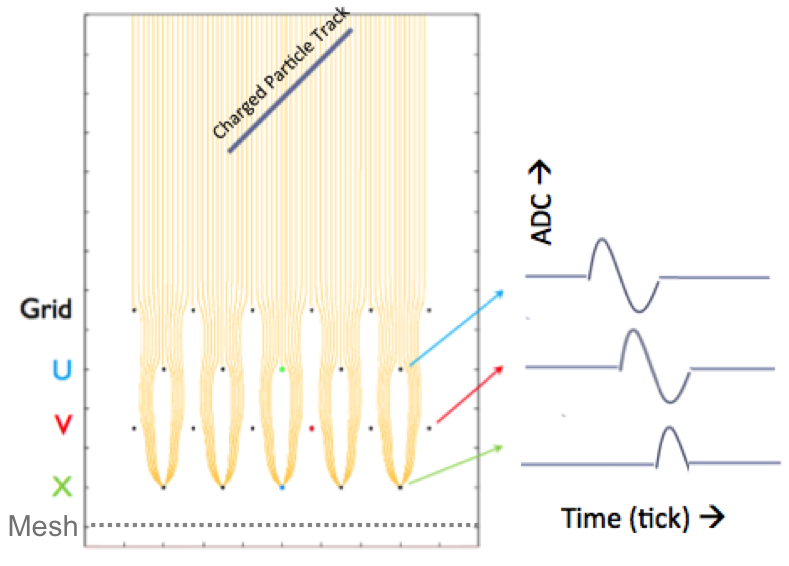
\includegraphics[width=0.9\linewidth]{sp-apa-drawing-wire-field-signals.png}
\captionof{figure}{Field lines and resulting signal shapes on the APA induction and collection wires.}
\label{fig:apa-fields}
\end{minipage}
\end{table}

\item \textbf{Wire type and tension}  The wire selected for the \dwords{apa} is \SI{152}{$\mu$m} beryllium (\num{1.9}\%) copper wire, %\footnote{\url{http://www.lfa-wire.com/heat-treatable-alloy-25_c17200-and-c17300.htm}}
chosen for its mechanical and electrical properties, ease of soldering, and cost.  The tension on the wires, combined with intermediate support combs (described in Section~\ref{sec:combs}) on the \dword{apa} frame cross beams, ensure that the wires are held taut in place with minimal sag.  Wire sag can affect the precision of reconstruction, as well as the transparency of the \dword{tpc} wire planes.  The tension must be low enough that when the wires are cooled, which increases their tension due to thermal contraction, they stay safely below the break load of the beryllium copper wire.  A tension of $6\pm$\SI{1}{N} is the baseline for \dword{dune}, to be confirmed after \dword{pdsp} analysis is completed.  To further mitigate wire slippage and its effect on detector performance, each wire in the \dword{apa} is anchored twice at all end points with both solder and epoxy.  See Section~\ref{sec:fdsp-apa-wires} for more details about the wires.

\end{itemize}

Table~\ref{tab:apaparameters} summarizes some of the principal design parameters for the \dword{spmod} 
\dwords{apa}.

\begin{dunetable}[APA design parameters]{lr}{tab:apaparameters}
{\dword{apa} design parameters}   
Parameter & Value  \\ \toprowrule
Active height & \SI{5.984}{m} \\ \colhline
Active width & \SI{2.300}{m} \\ \colhline
Wire pitch ($U,V$) & \uvpitch \\ \colhline
Wire pitch ($X,G$) & \xgpitch \\ \colhline
Wire pitch tolerance & \wirepitchtol \\ \colhline
Wire plane spacing & \planespace \\ \colhline
Wire plane spacing tolerance & $\pm$\SI{0.5}{mm} \\ \colhline
Wire Angle (w.r.t. vertical) ($U,V$) & \apainducwireangle{} \\ \colhline
Wire Angle (w.r.t. vertical) ($X,G$) & \apacollwireangle \\ \colhline
Number of wires / \dword{apa} & 960 ($X$), 960 ($G$), 800 ($U$), 800 ($V$) \\ \colhline
Number of electronic channels / \dword{apa} & 2560 \\ \colhline
%Wire Tension & \SI{5.0}{N} \\ \colhline
%Wire Tension Tolerance & $\pm$\SI{1}{N} \\ \colhline
Wire material & beryllium copper \\ \colhline
Wire diameter & 152 $\mu$m \\ \colhline
%Wire Resistivity & 7.68 $\mu\Omega$-cm $@$ 20$^{\circ}$ C \\ \colhline
%Wire Resistance/m & 4.4 $\Omega$/m $@$ 20$^{\circ}$ C \\ \colhline
%Frame Planarity & 5 mm \\ \colhline
%Photon Detector Slots & 10 \\
\end{dunetable}


%%%%%%%%%%%%%%%%%%%%%%%%%%%%%%%%%%%%%%%%%%%%%%%%%%%%%%%%%%%%%%%%%%%%%%
\subsection{Support Frames}
\label{sec:fdsp-apa-frames}

The \dword{apa} frames are built of rectangular hollow section (RHS) stainless steel tubes.  Figure~\ref{fig:apa-frame-full} shows three long tubes, a foot tube, a head tube, and eight cross-piece ribs that bolt together to create the \SI{6.0}{m} tall by \SI{2.3}{m} wide frame. All hollow sections are \SI{10.2}{cm} (\SI{4}{in}) deep with varying widths depending on their role. % (see Figures~\ref{fig:apa-frame-full} and \ref{fig:apa-frame-details}).

%\begin{dunefigure}[Bare \dword{apa} frame drawing]{fig:apa-frame-2}
%{A \dword{pdsp} \dword{apa} frame showing overall dimensions and the \num{13} separate stainless steel tube sections that bolt together to form a complete frame.  The long tubes and foot tube are a \num{4}$\times$\SI{4}{in} cross section, the head tube is \num{4}$\times$\SI{6}{in}, and the ribs are \num{4}$\times$\SI{2}{in}. Also shown are the slots and guide rails used to house the light guide bar \dwords{pd}.}% in \dword{pdsp}.}
%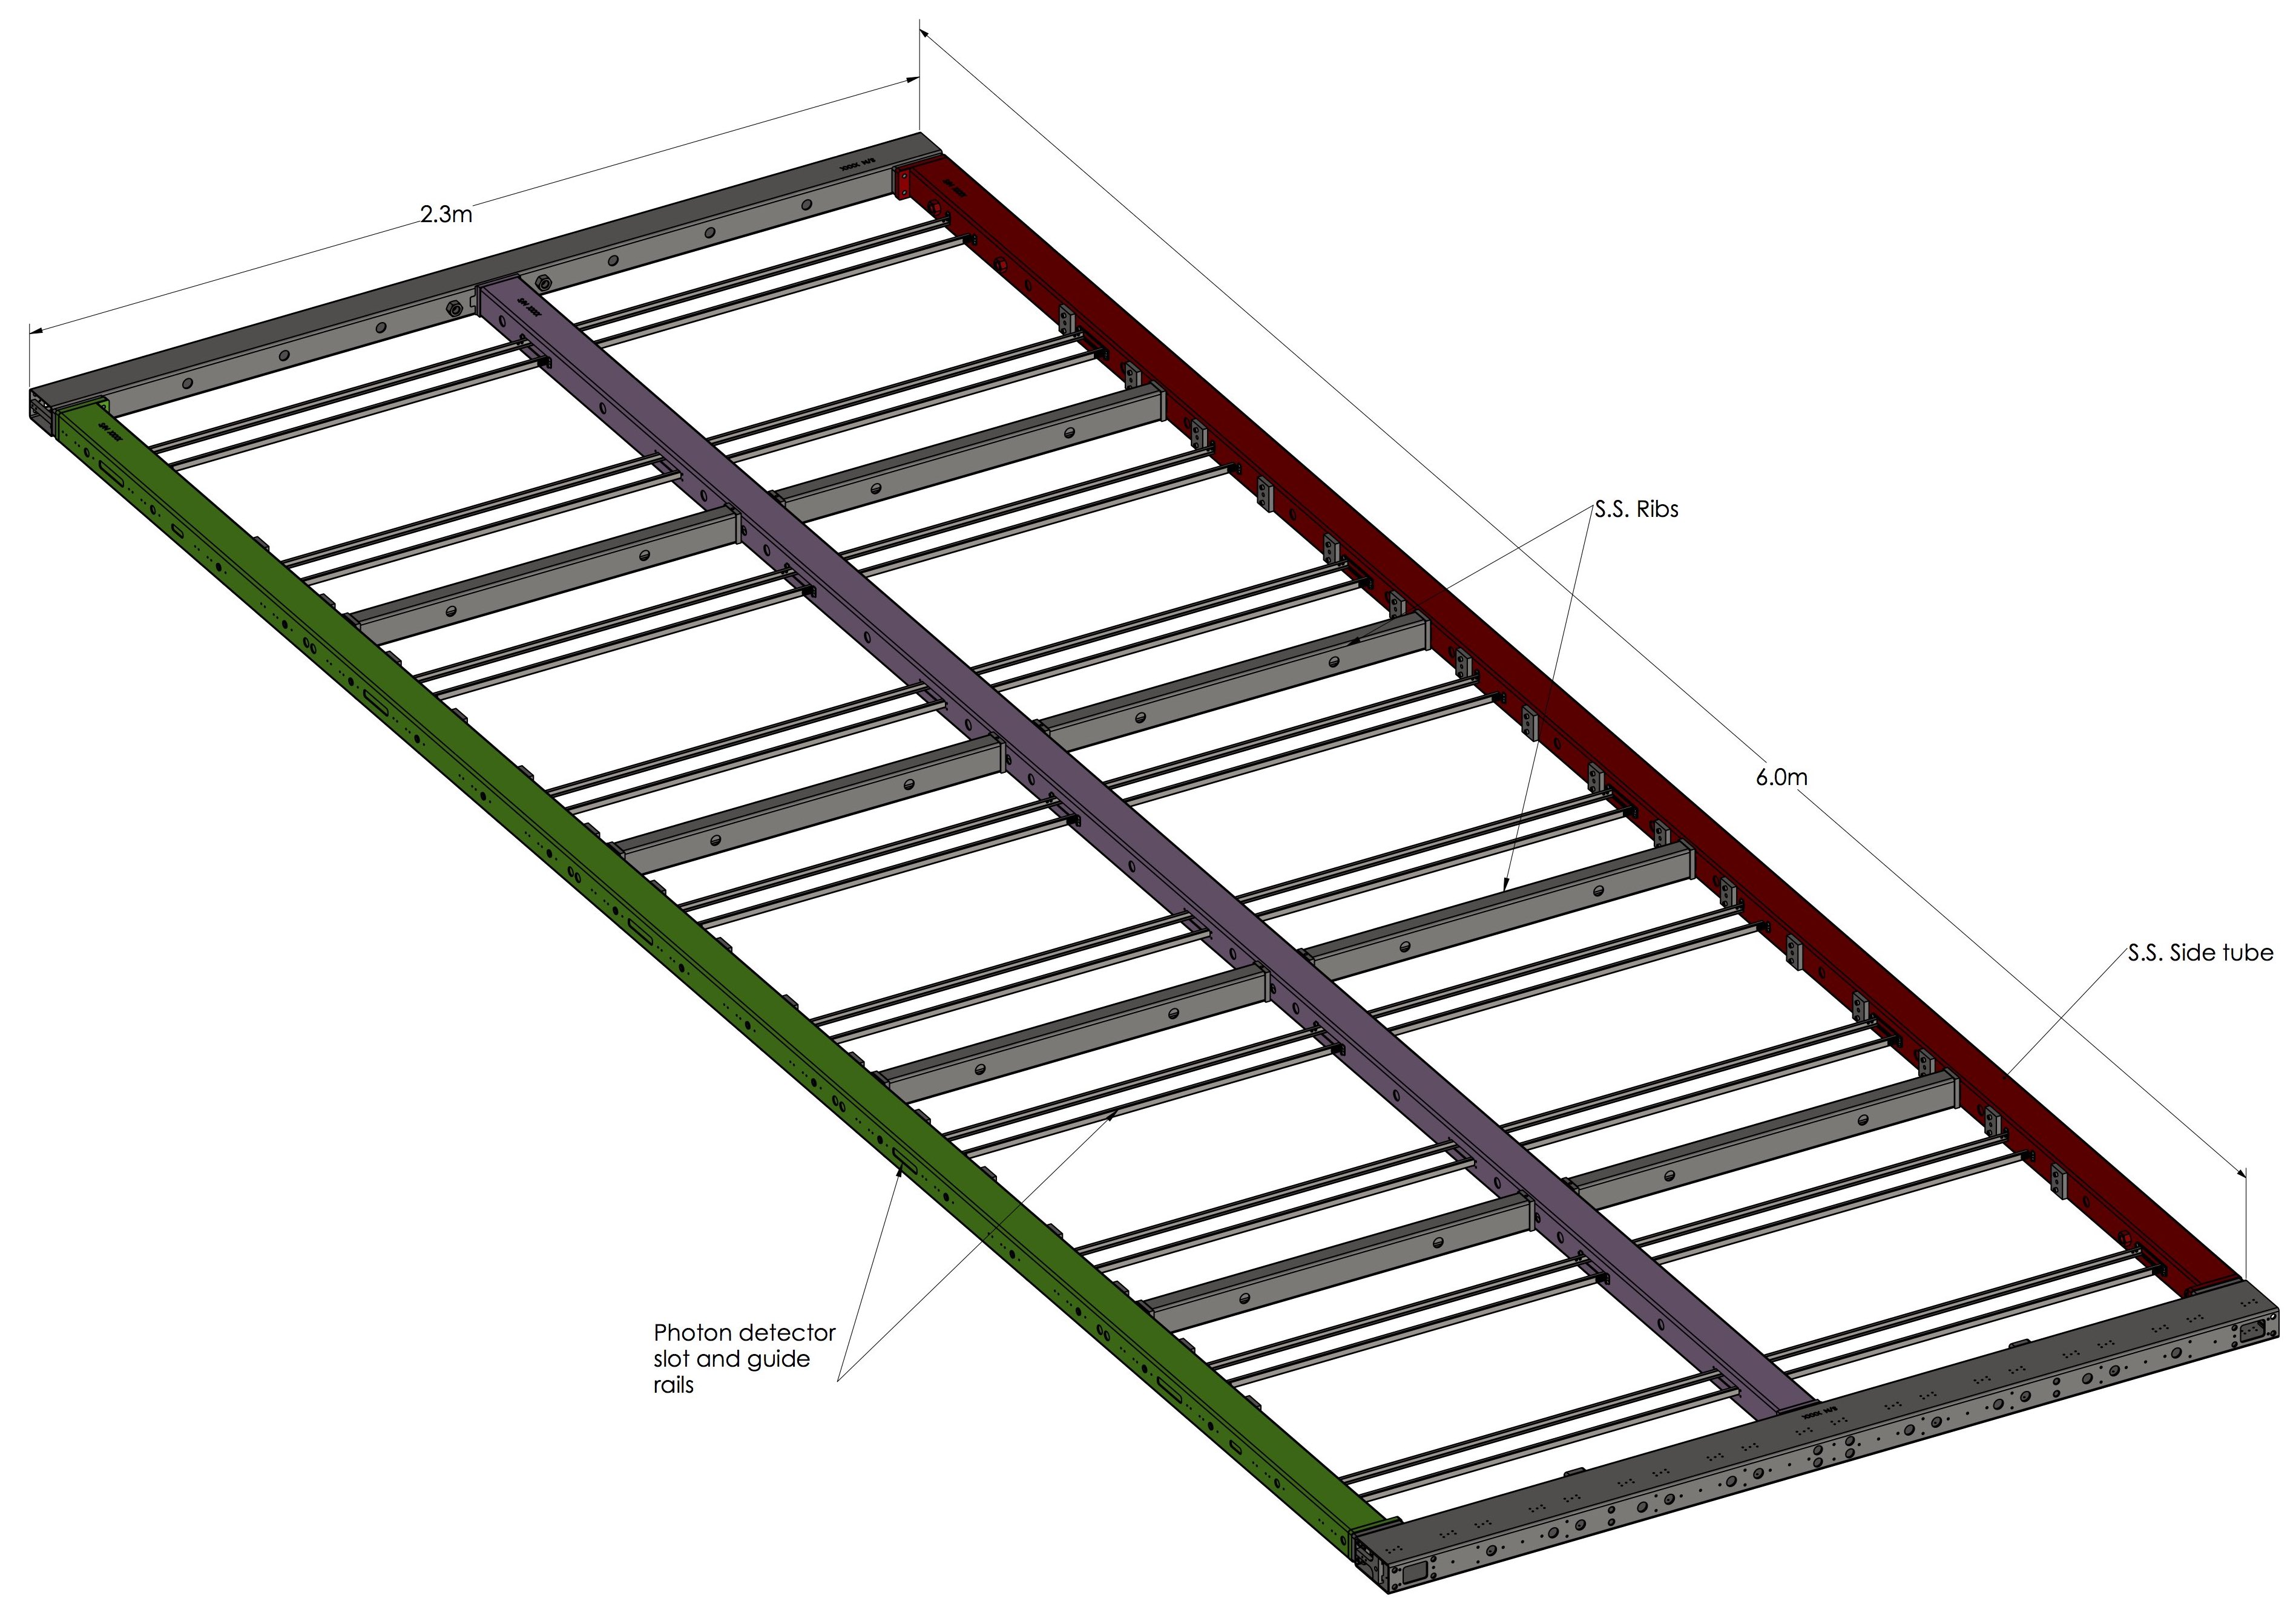
\includegraphics[width=0.9\textwidth]{sp-apa-iso-color.jpg} 
%\end{dunefigure}

\begin{dunefigure}[Bare APA frame drawings]{fig:apa-frame-full}
{Top: A \dword{dune} \dword{apa} frame showing the \num{13} separate stainless steel tube sections that bolt together to form a complete frame.  The long tubes and foot tube are a \num{10.2}$\times$\SI{10.2}{cm} (\num{4}$\times$\SI{4}{inch}) cross section, the head tube is \num{10.2}$\times$\SI{15.2}{cm} (\num{4}$\times$\SI{6}{inch}), and the ribs are \num{10.2}$\times$\SI{5.1}{cm} (\num{4}$\times$\SI{2}{inch}). %Lower Left: The corner joint between the foot tube and the side tube. Lower Middle: The joint between the side tube and a rib. Lower Right: The joints between the head tube and the side and center tubes.
}
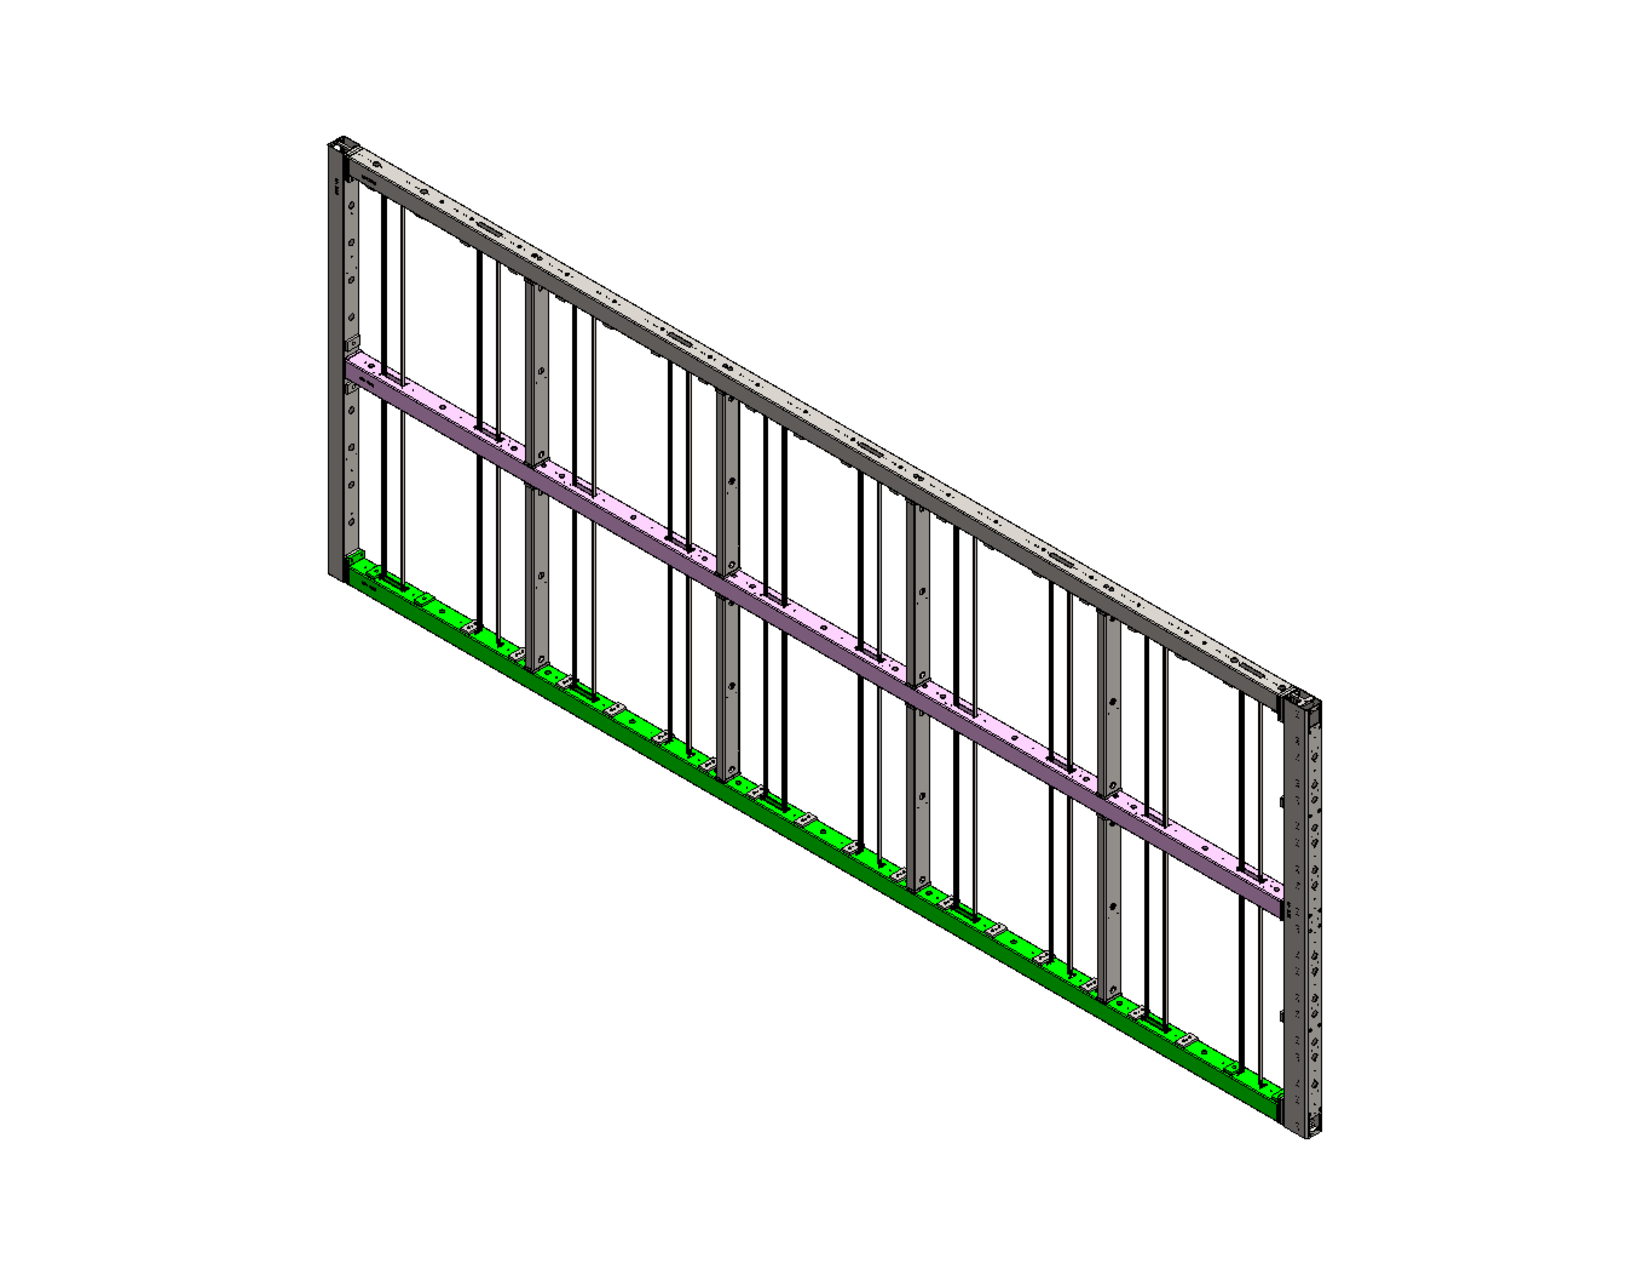
\includegraphics[width=1\textwidth]{sp-apa-frame-full-2.pdf}
%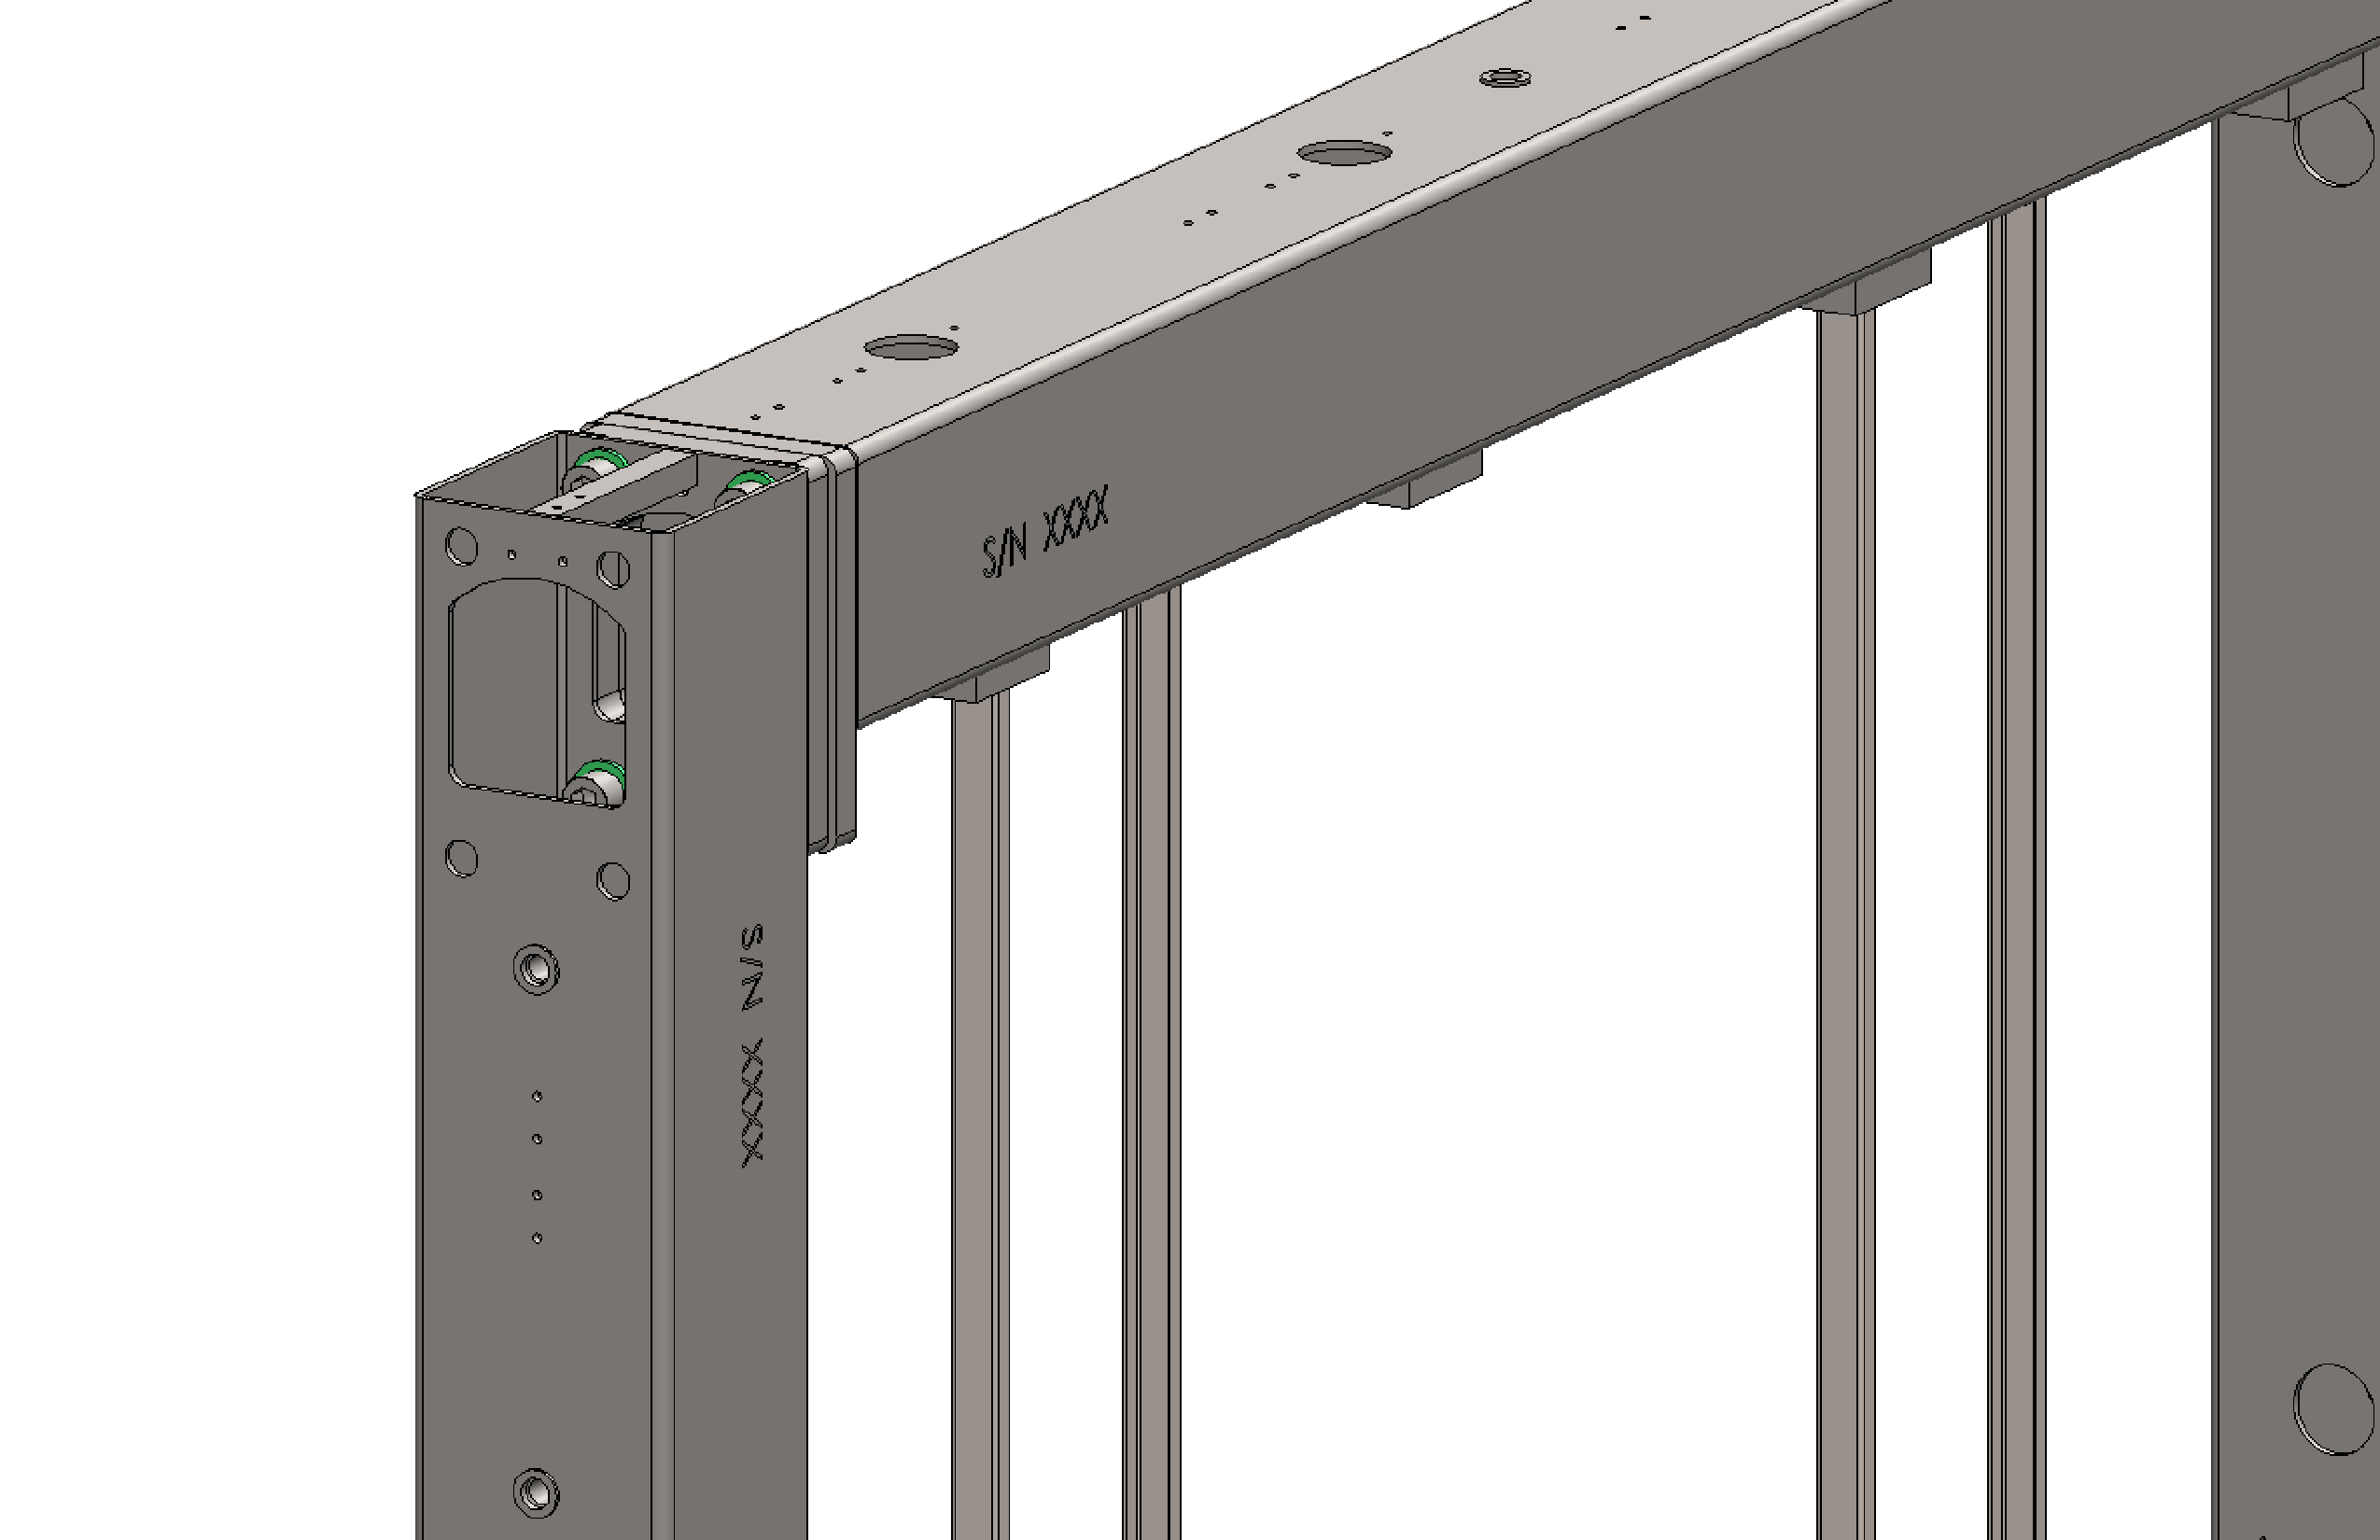
\includegraphics[height=0.34\textheight,trim=0mm 0mm 0mm 0mm,clip]{sp-apa-frame-foot.pdf}
%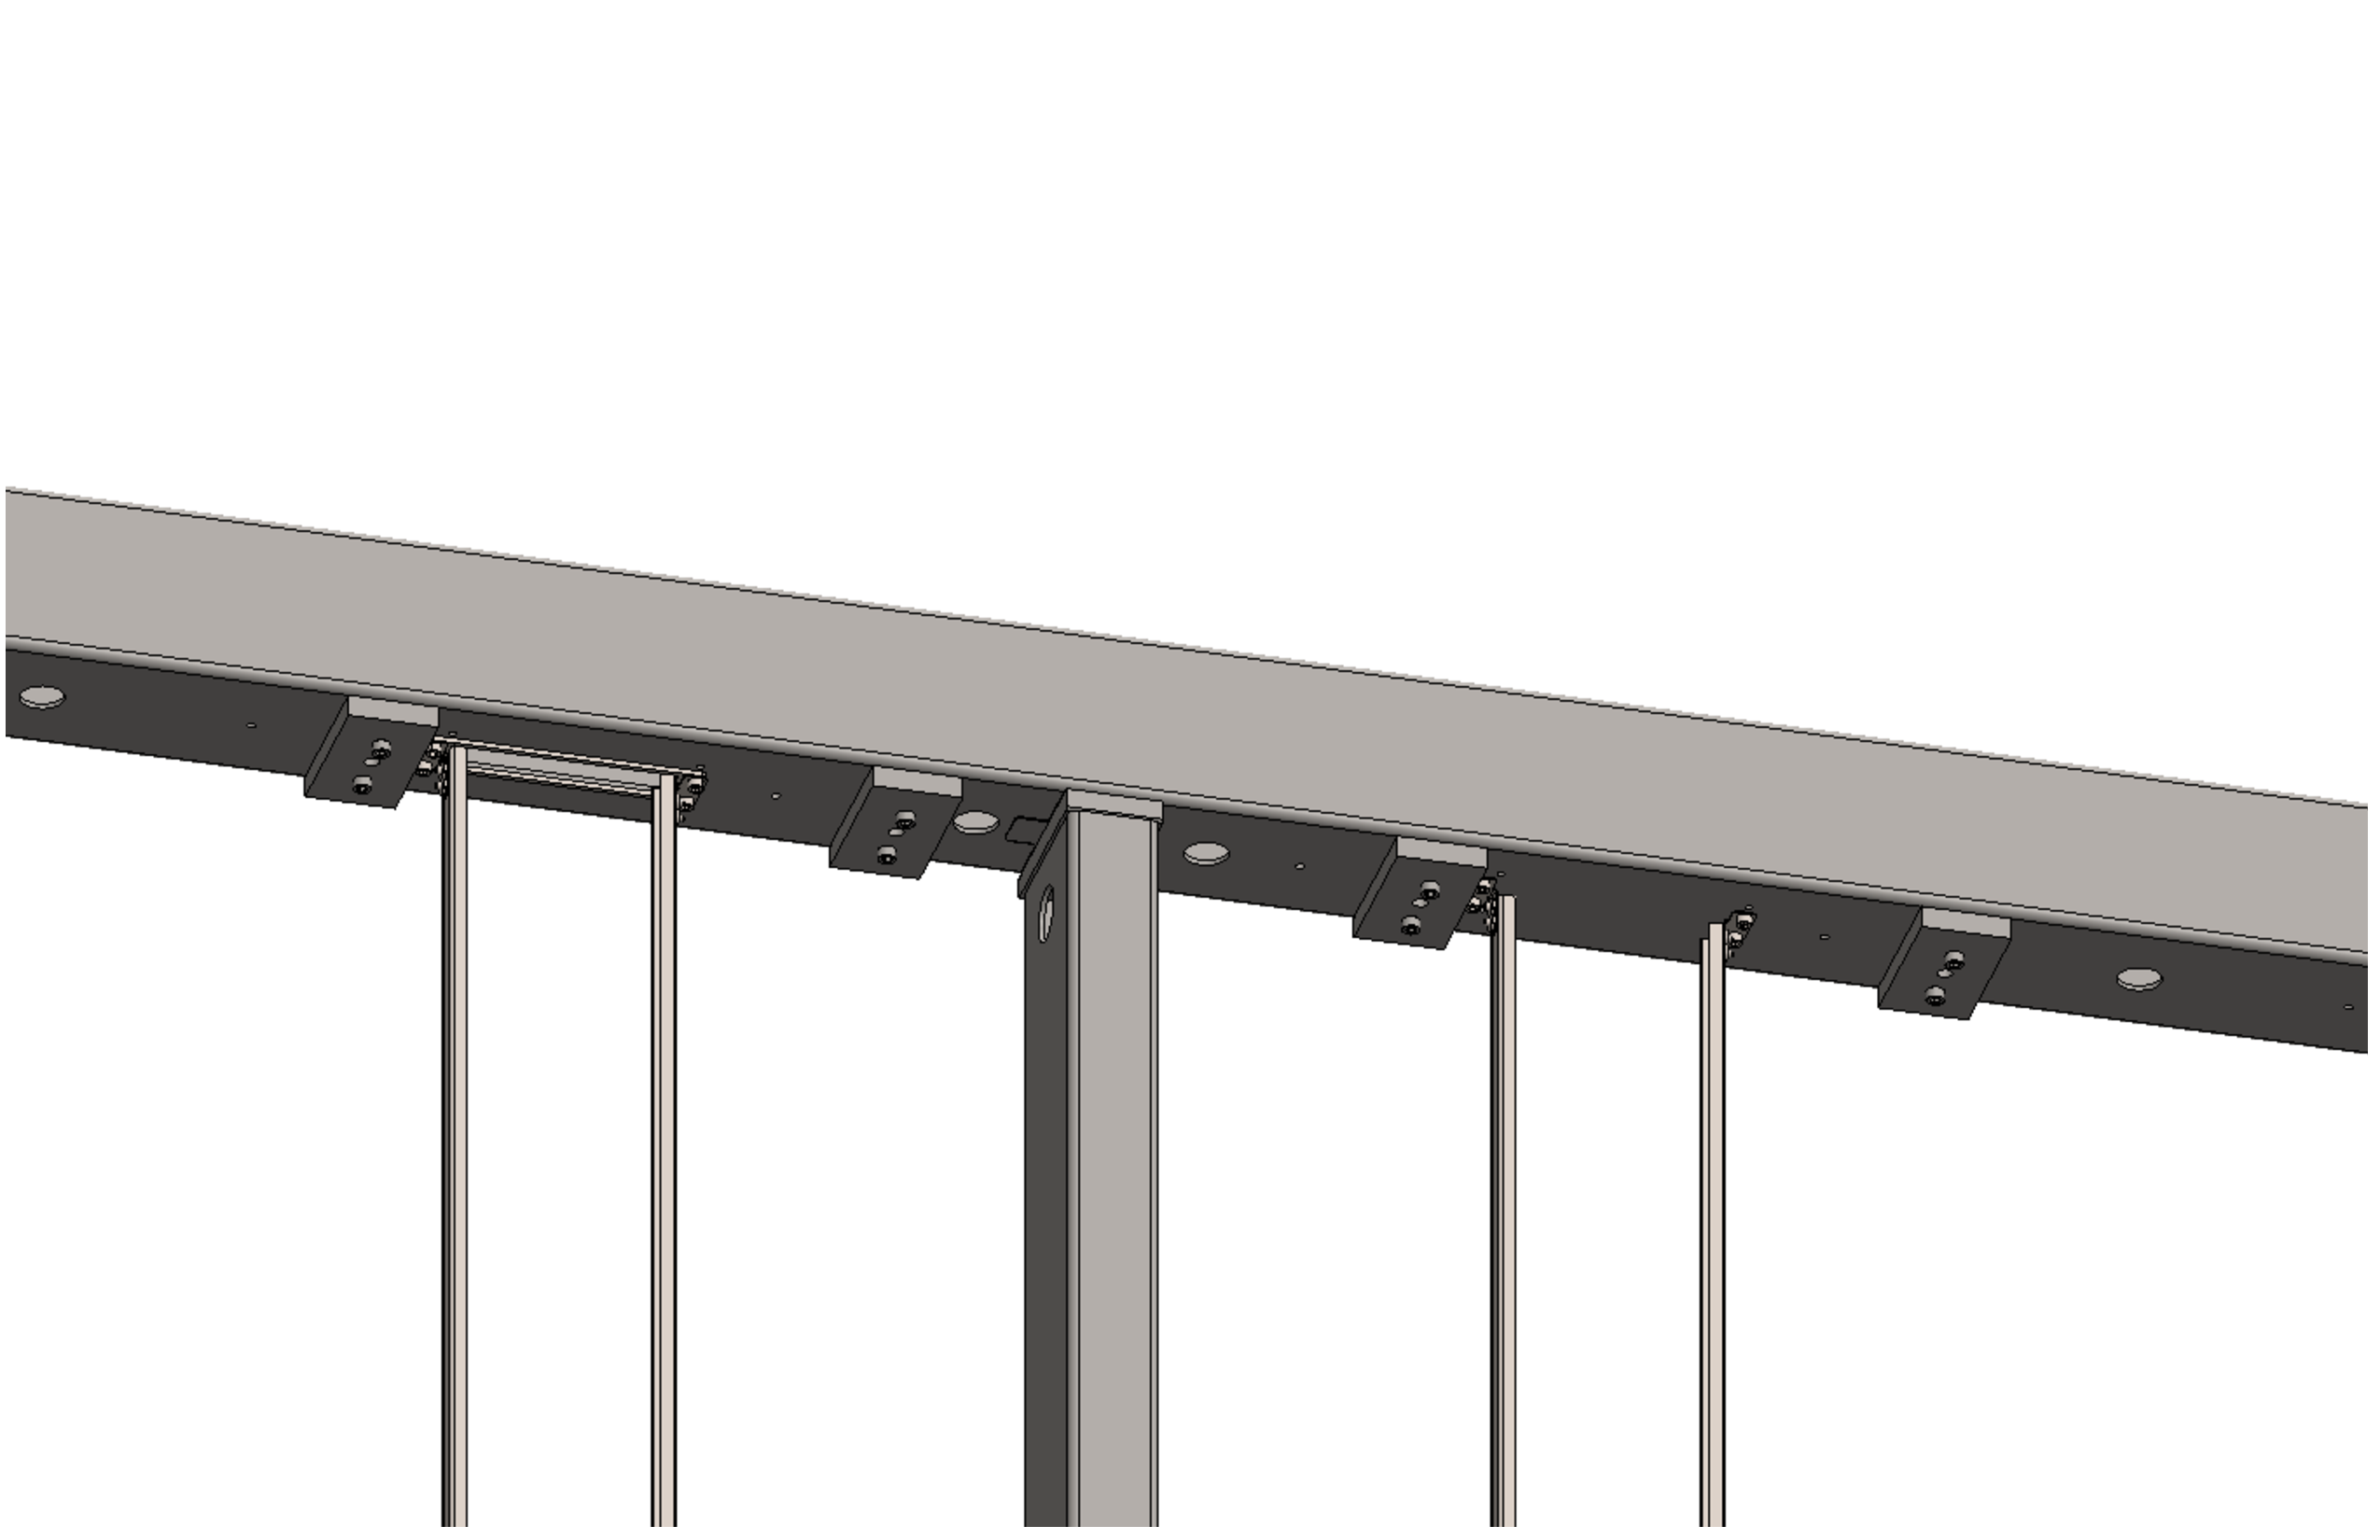
\includegraphics[height=0.34\textheight,trim=0mm 0mm 0mm 0mm,clip]{sp-apa-frame-side-joint.pdf}
%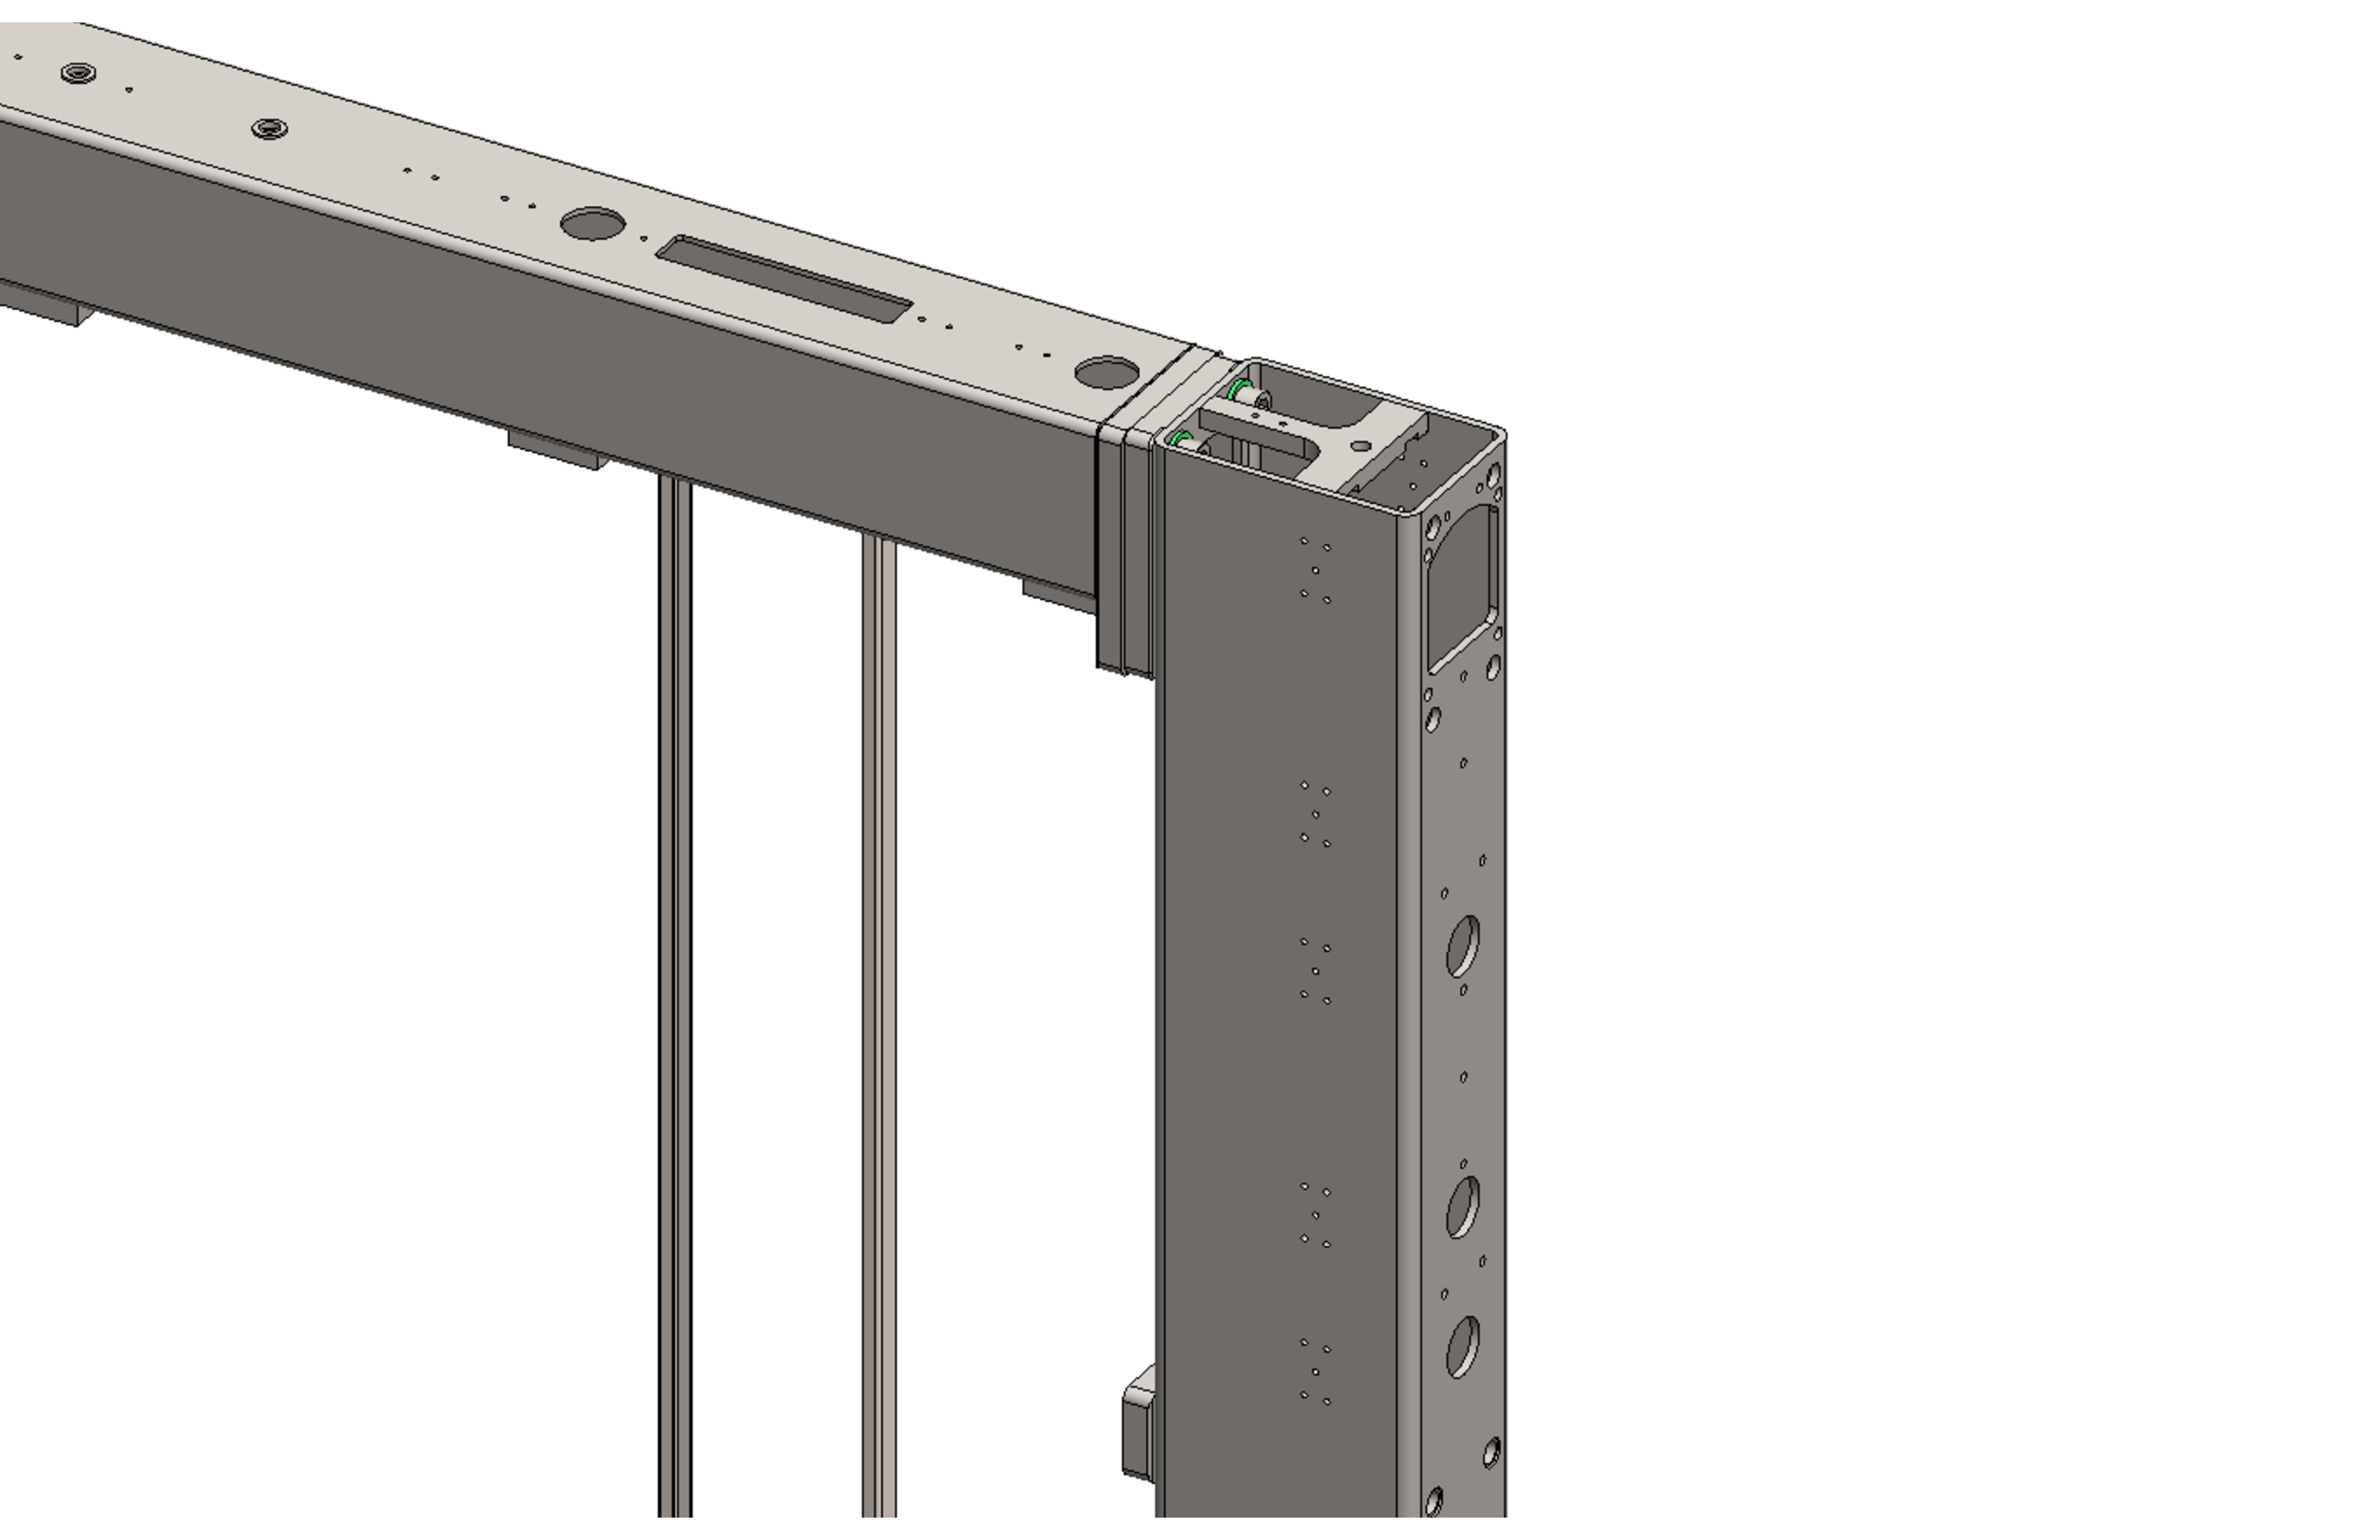
\includegraphics[height=0.34\textheight]{sp-apa-frame-head.pdf}
\end{dunefigure}

\begin{dunefigure}[Bare APA frame drawings]{fig:apa-frame-details}
{\dword{apa} frame construction details. Top: The corner joint between the foot tube and the side tube. Middle: The joint between the side tube and a rib. Lower Bottom: The joint between the head tube and the side tube.}
%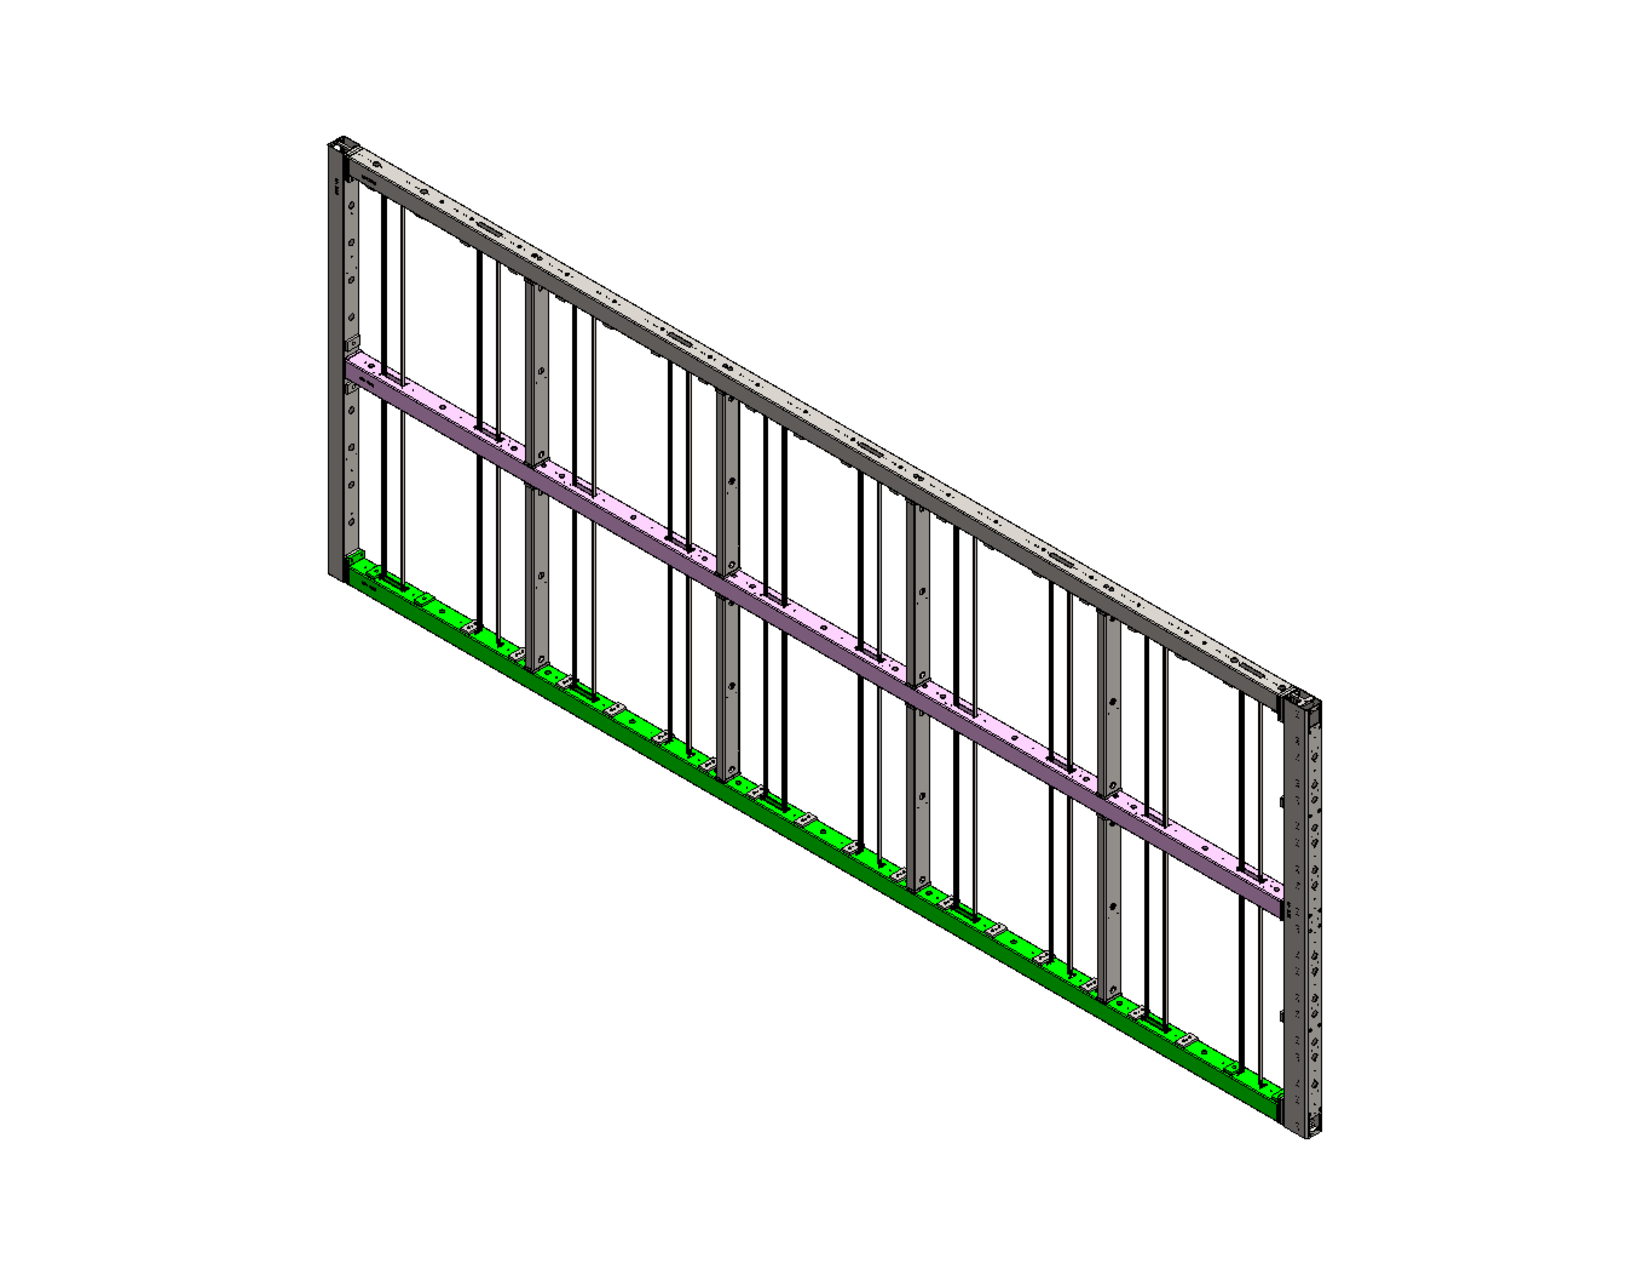
\includegraphics[width=1\textwidth]{sp-apa-frame-full-2.pdf}
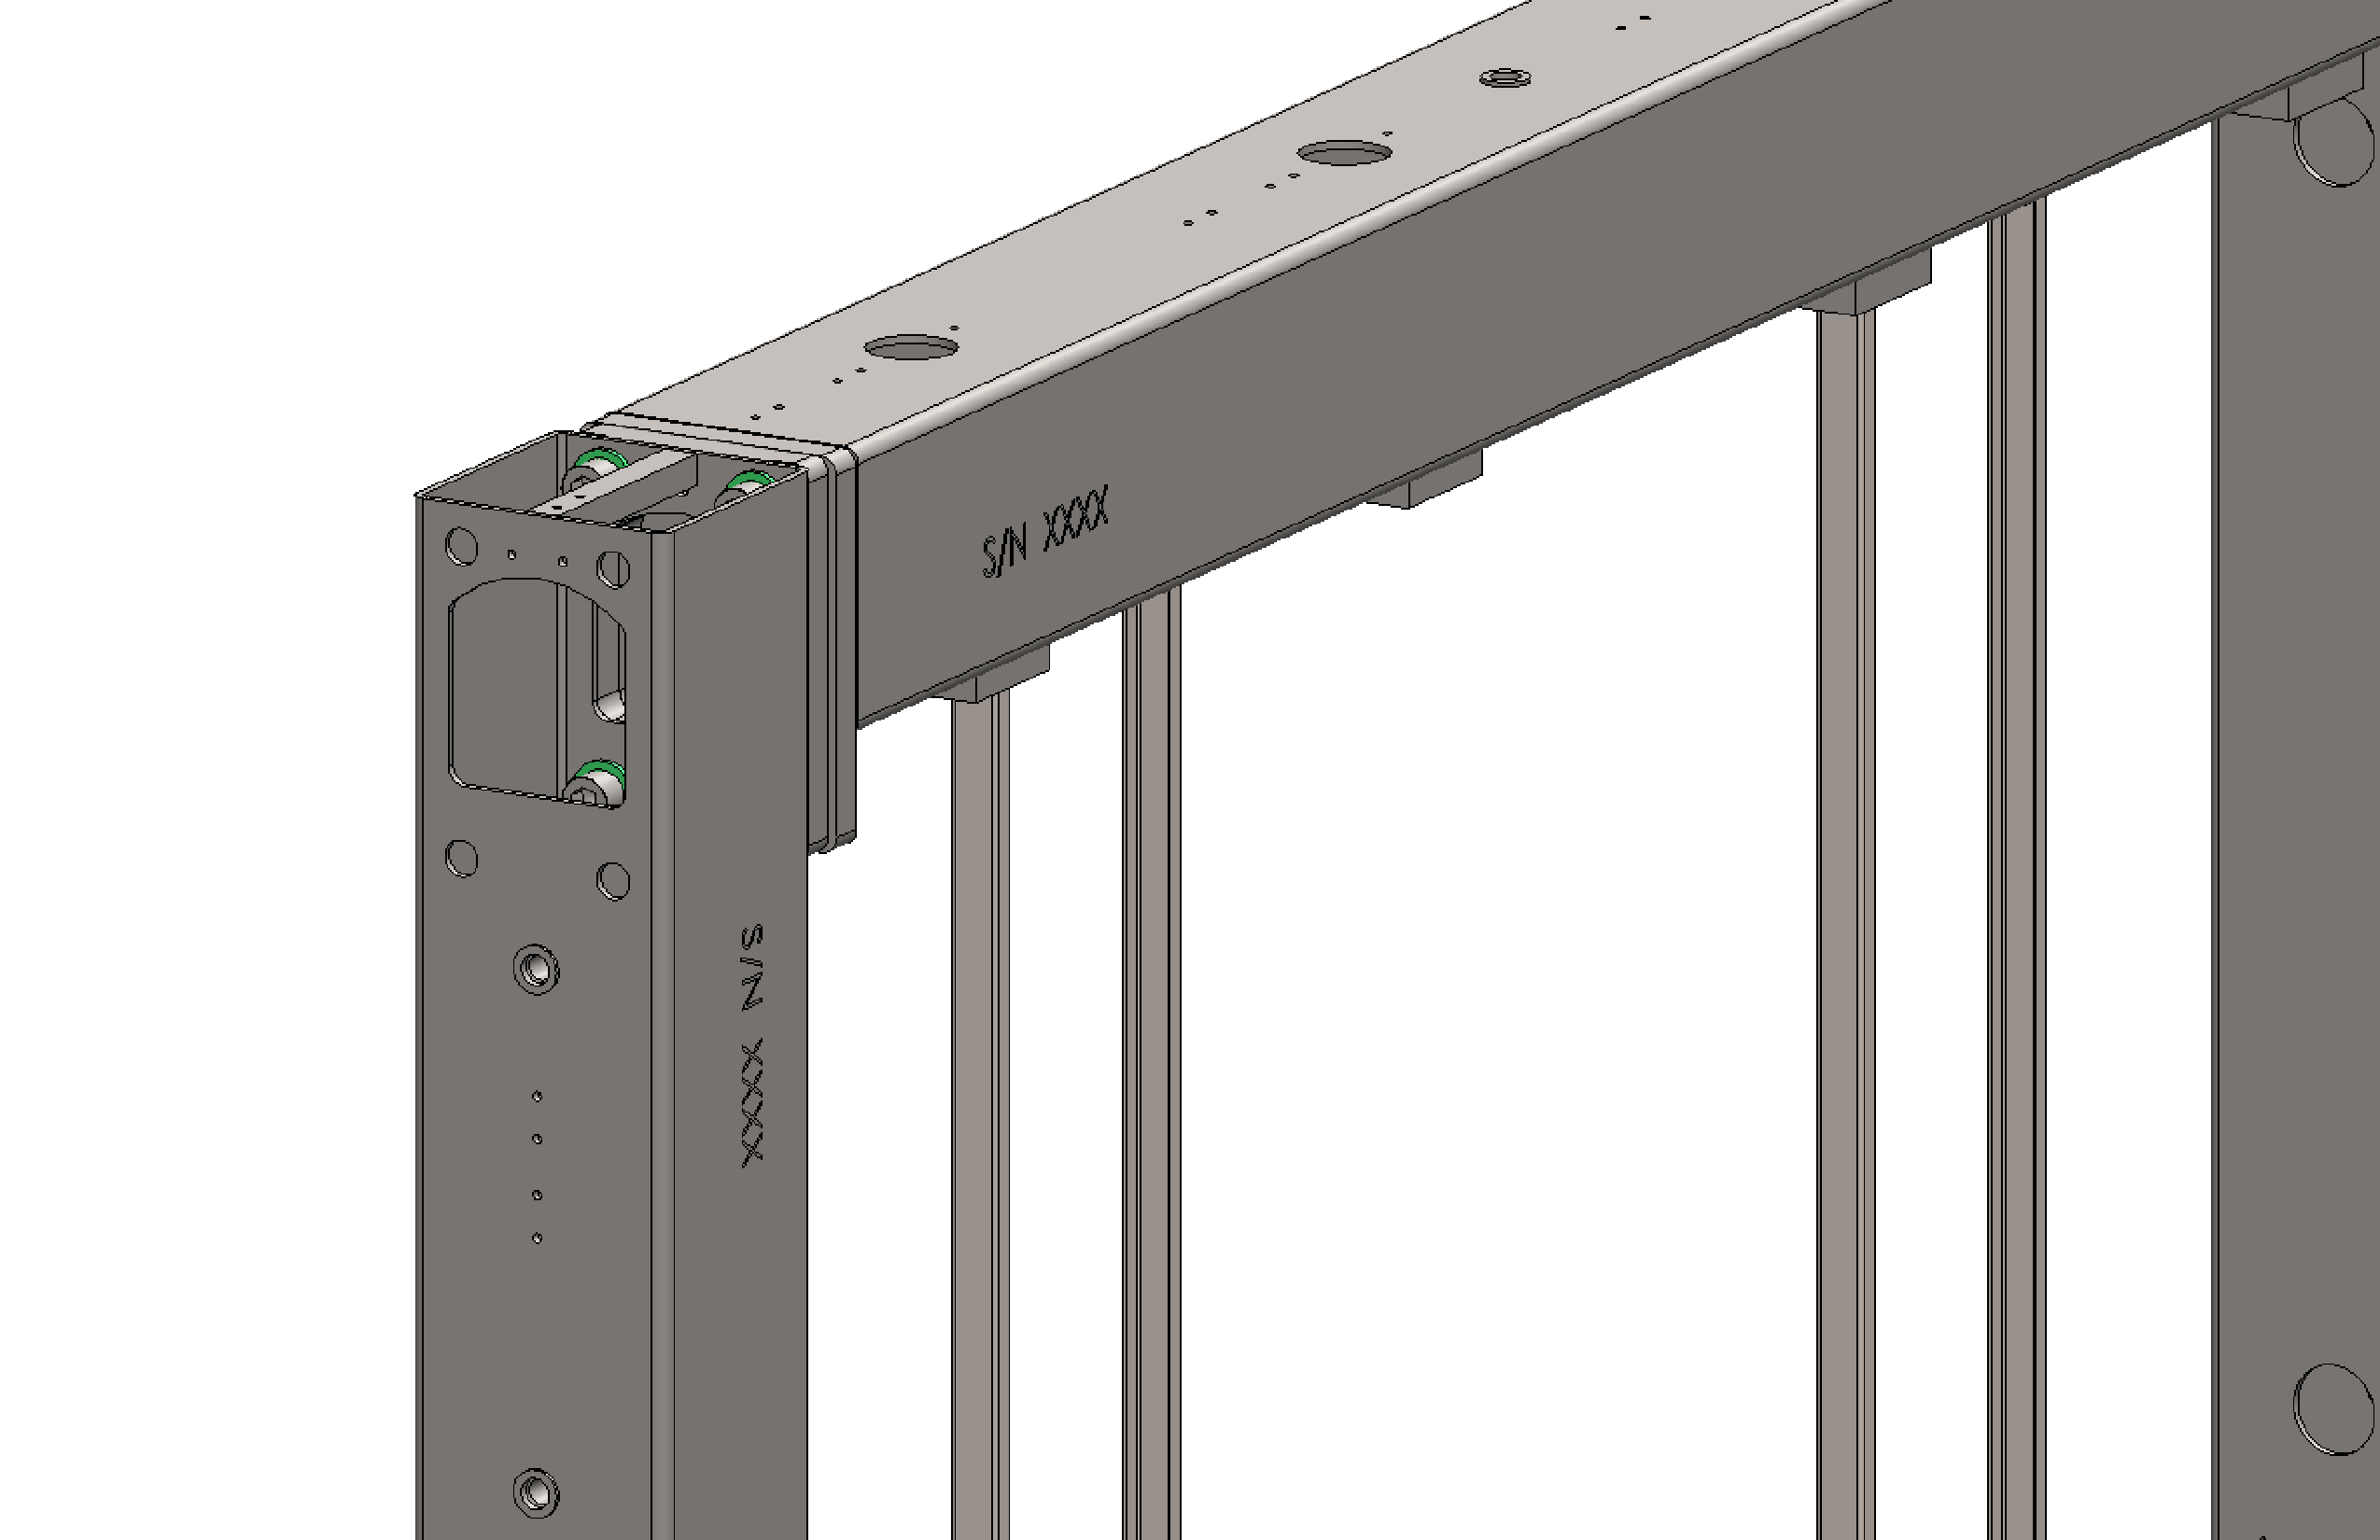
\includegraphics[height=0.31\textheight,trim=0mm 0mm 0mm 0mm,clip]{sp-apa-frame-foot.pdf}
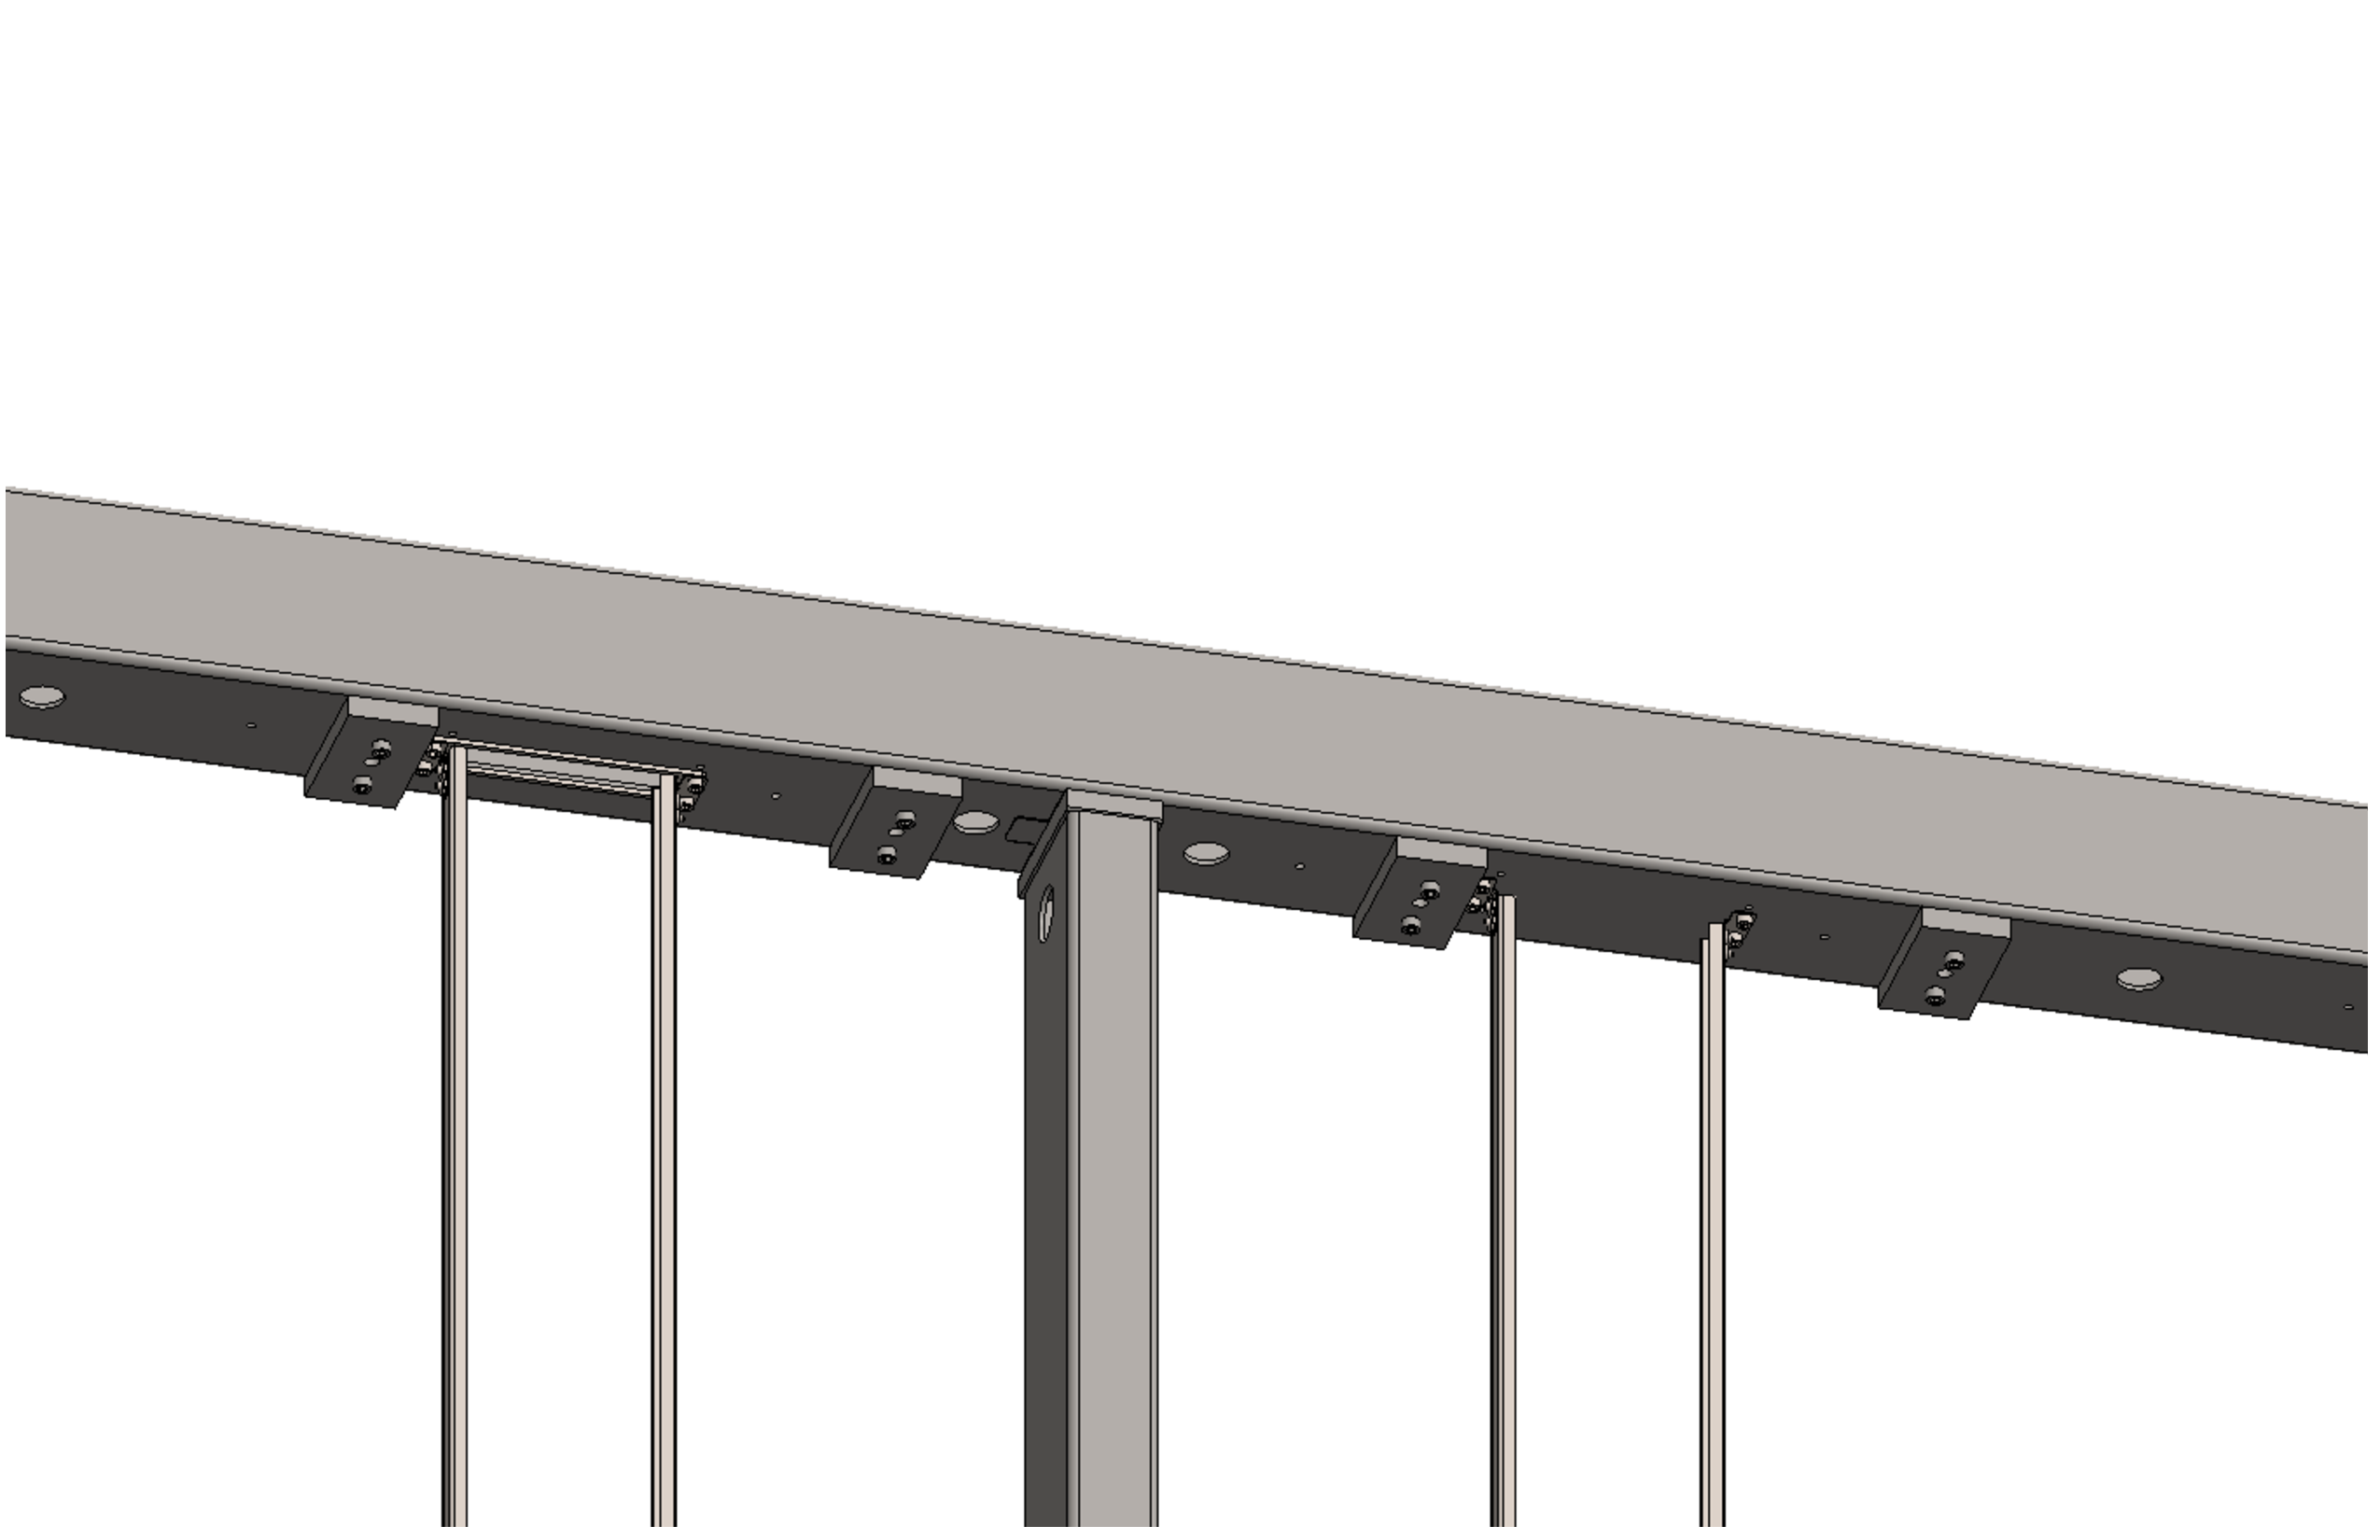
\includegraphics[height=0.28\textheight,trim=0mm 0mm 0mm 0mm,clip]{sp-apa-frame-side-joint.pdf}
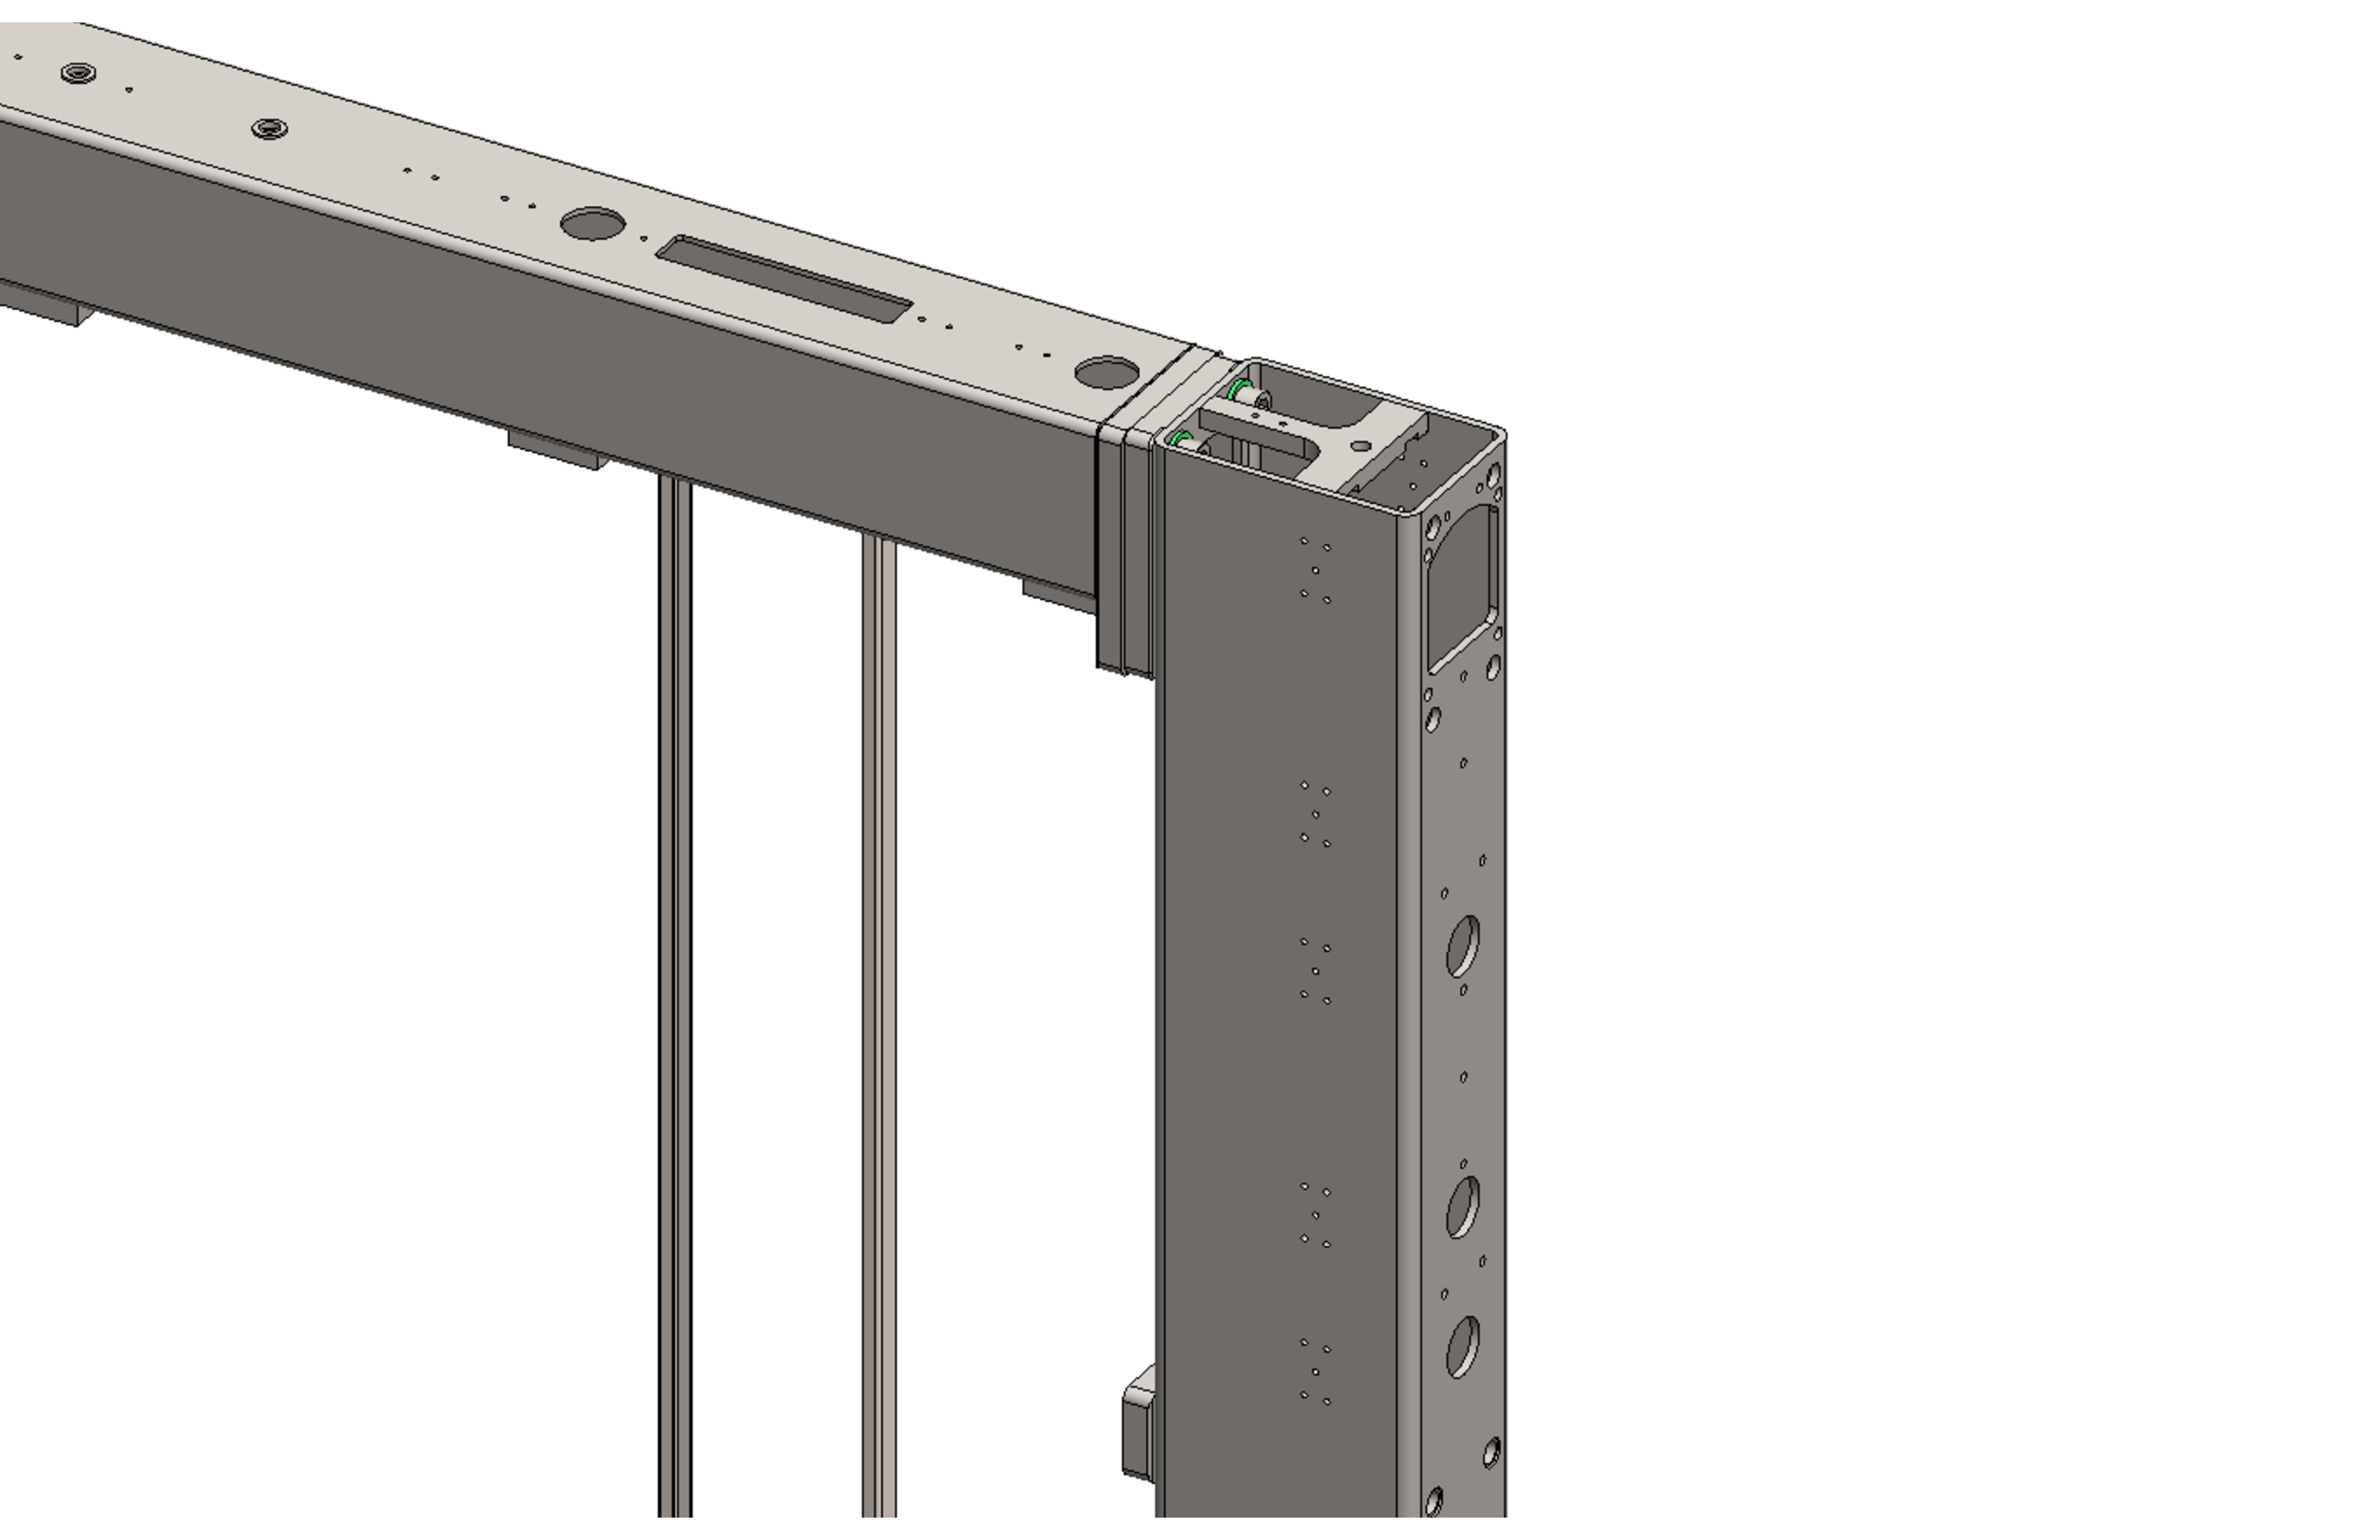
\includegraphics[height=0.32\textheight]{sp-apa-frame-head.pdf}
\end{dunefigure}

The head and foot tubes are bolted to the side and center pieces via abutment flanges welded to the tubes. In production, the pieces can be individually machined and cleaned before assembly to give flexibility both in the production process and help remain within the flatness and shape tolerances.  During final assembly, shims are used to create a flat, rectangular frame of the specified dimensions.  The central cross pieces are similarly attached to the side pieces.  Figure~\ref{fig:apa-frame-details} shows models of the different joints.   

%\begin{dunefigure}[Details of \dword{apa} bolted joints]{fig:tpc_apa_boltedjointdrawing}
%{The bolted joints in the \dword{apa} frame. Left: Connection between the head tube and a side tube. Right: Connections between the center tube and the rib pieces on either side.  These bolted connections can be shimmed during assembly to ensure the frame meets dimensional and flatness specifications. %\fixme{PSL: Need new versions of these drawings for the 4in frame}}
%}
%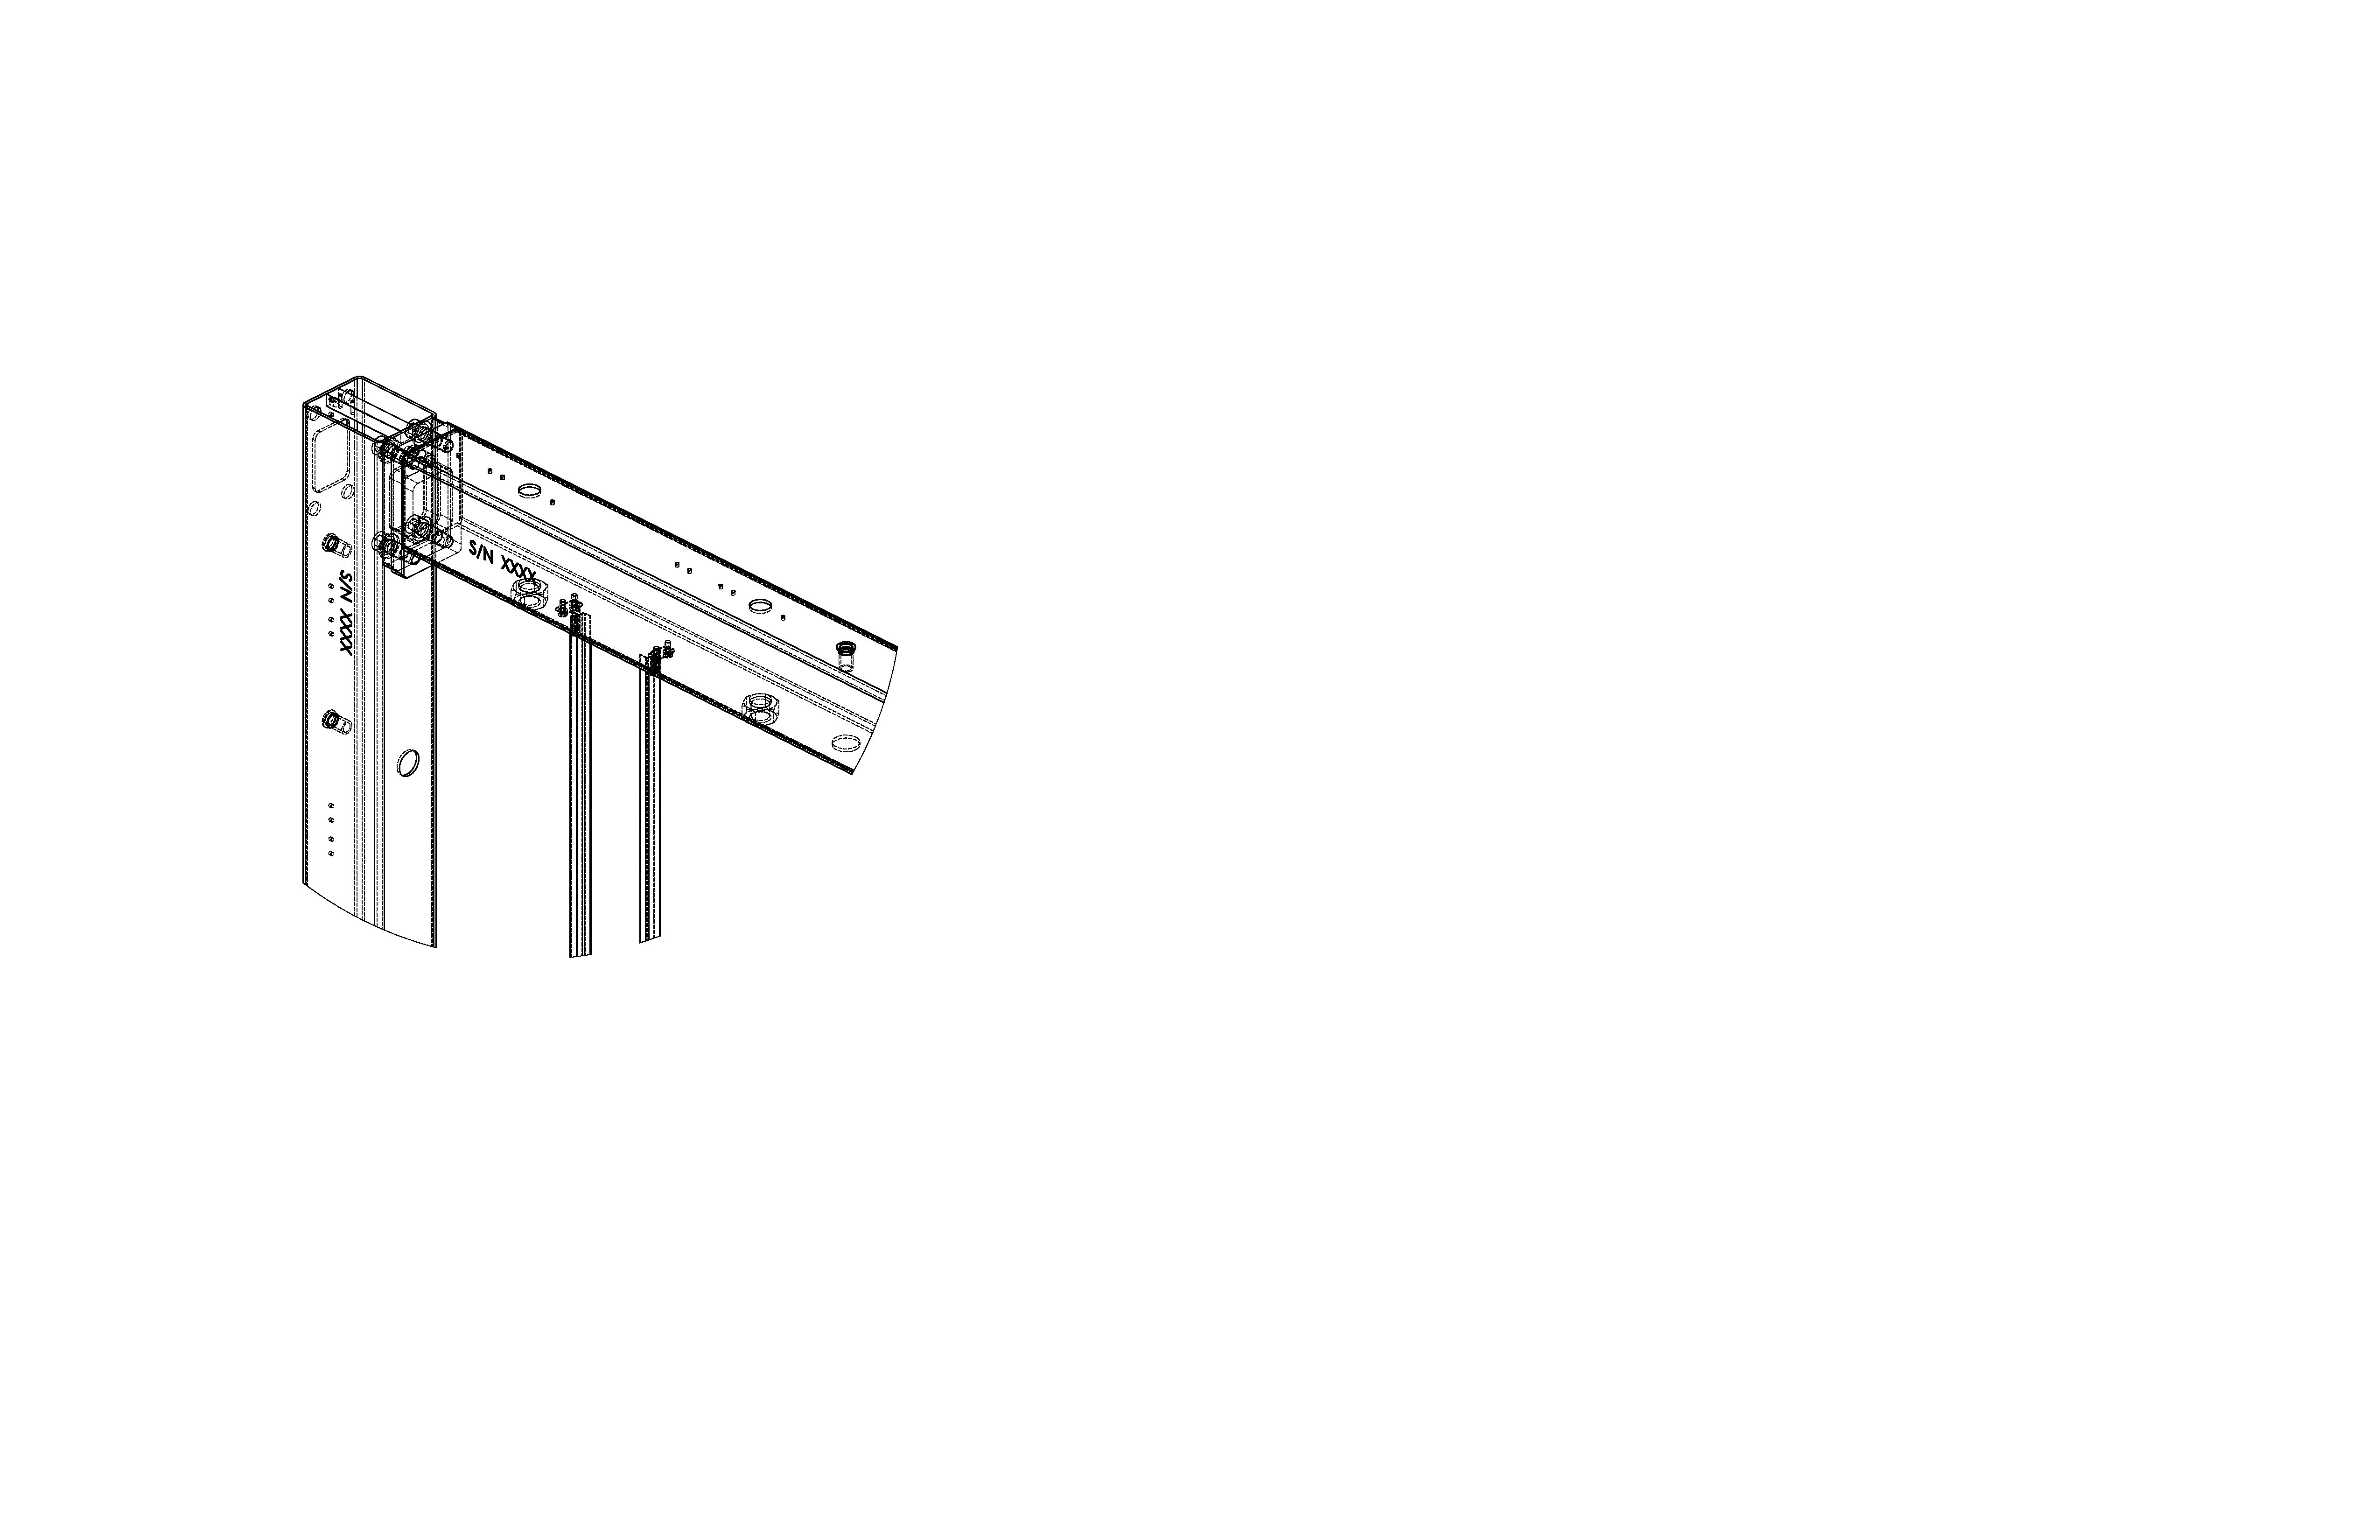
\includegraphics[width=0.45\textwidth]{sp-apa-joint-detail-1.pdf} \quad
%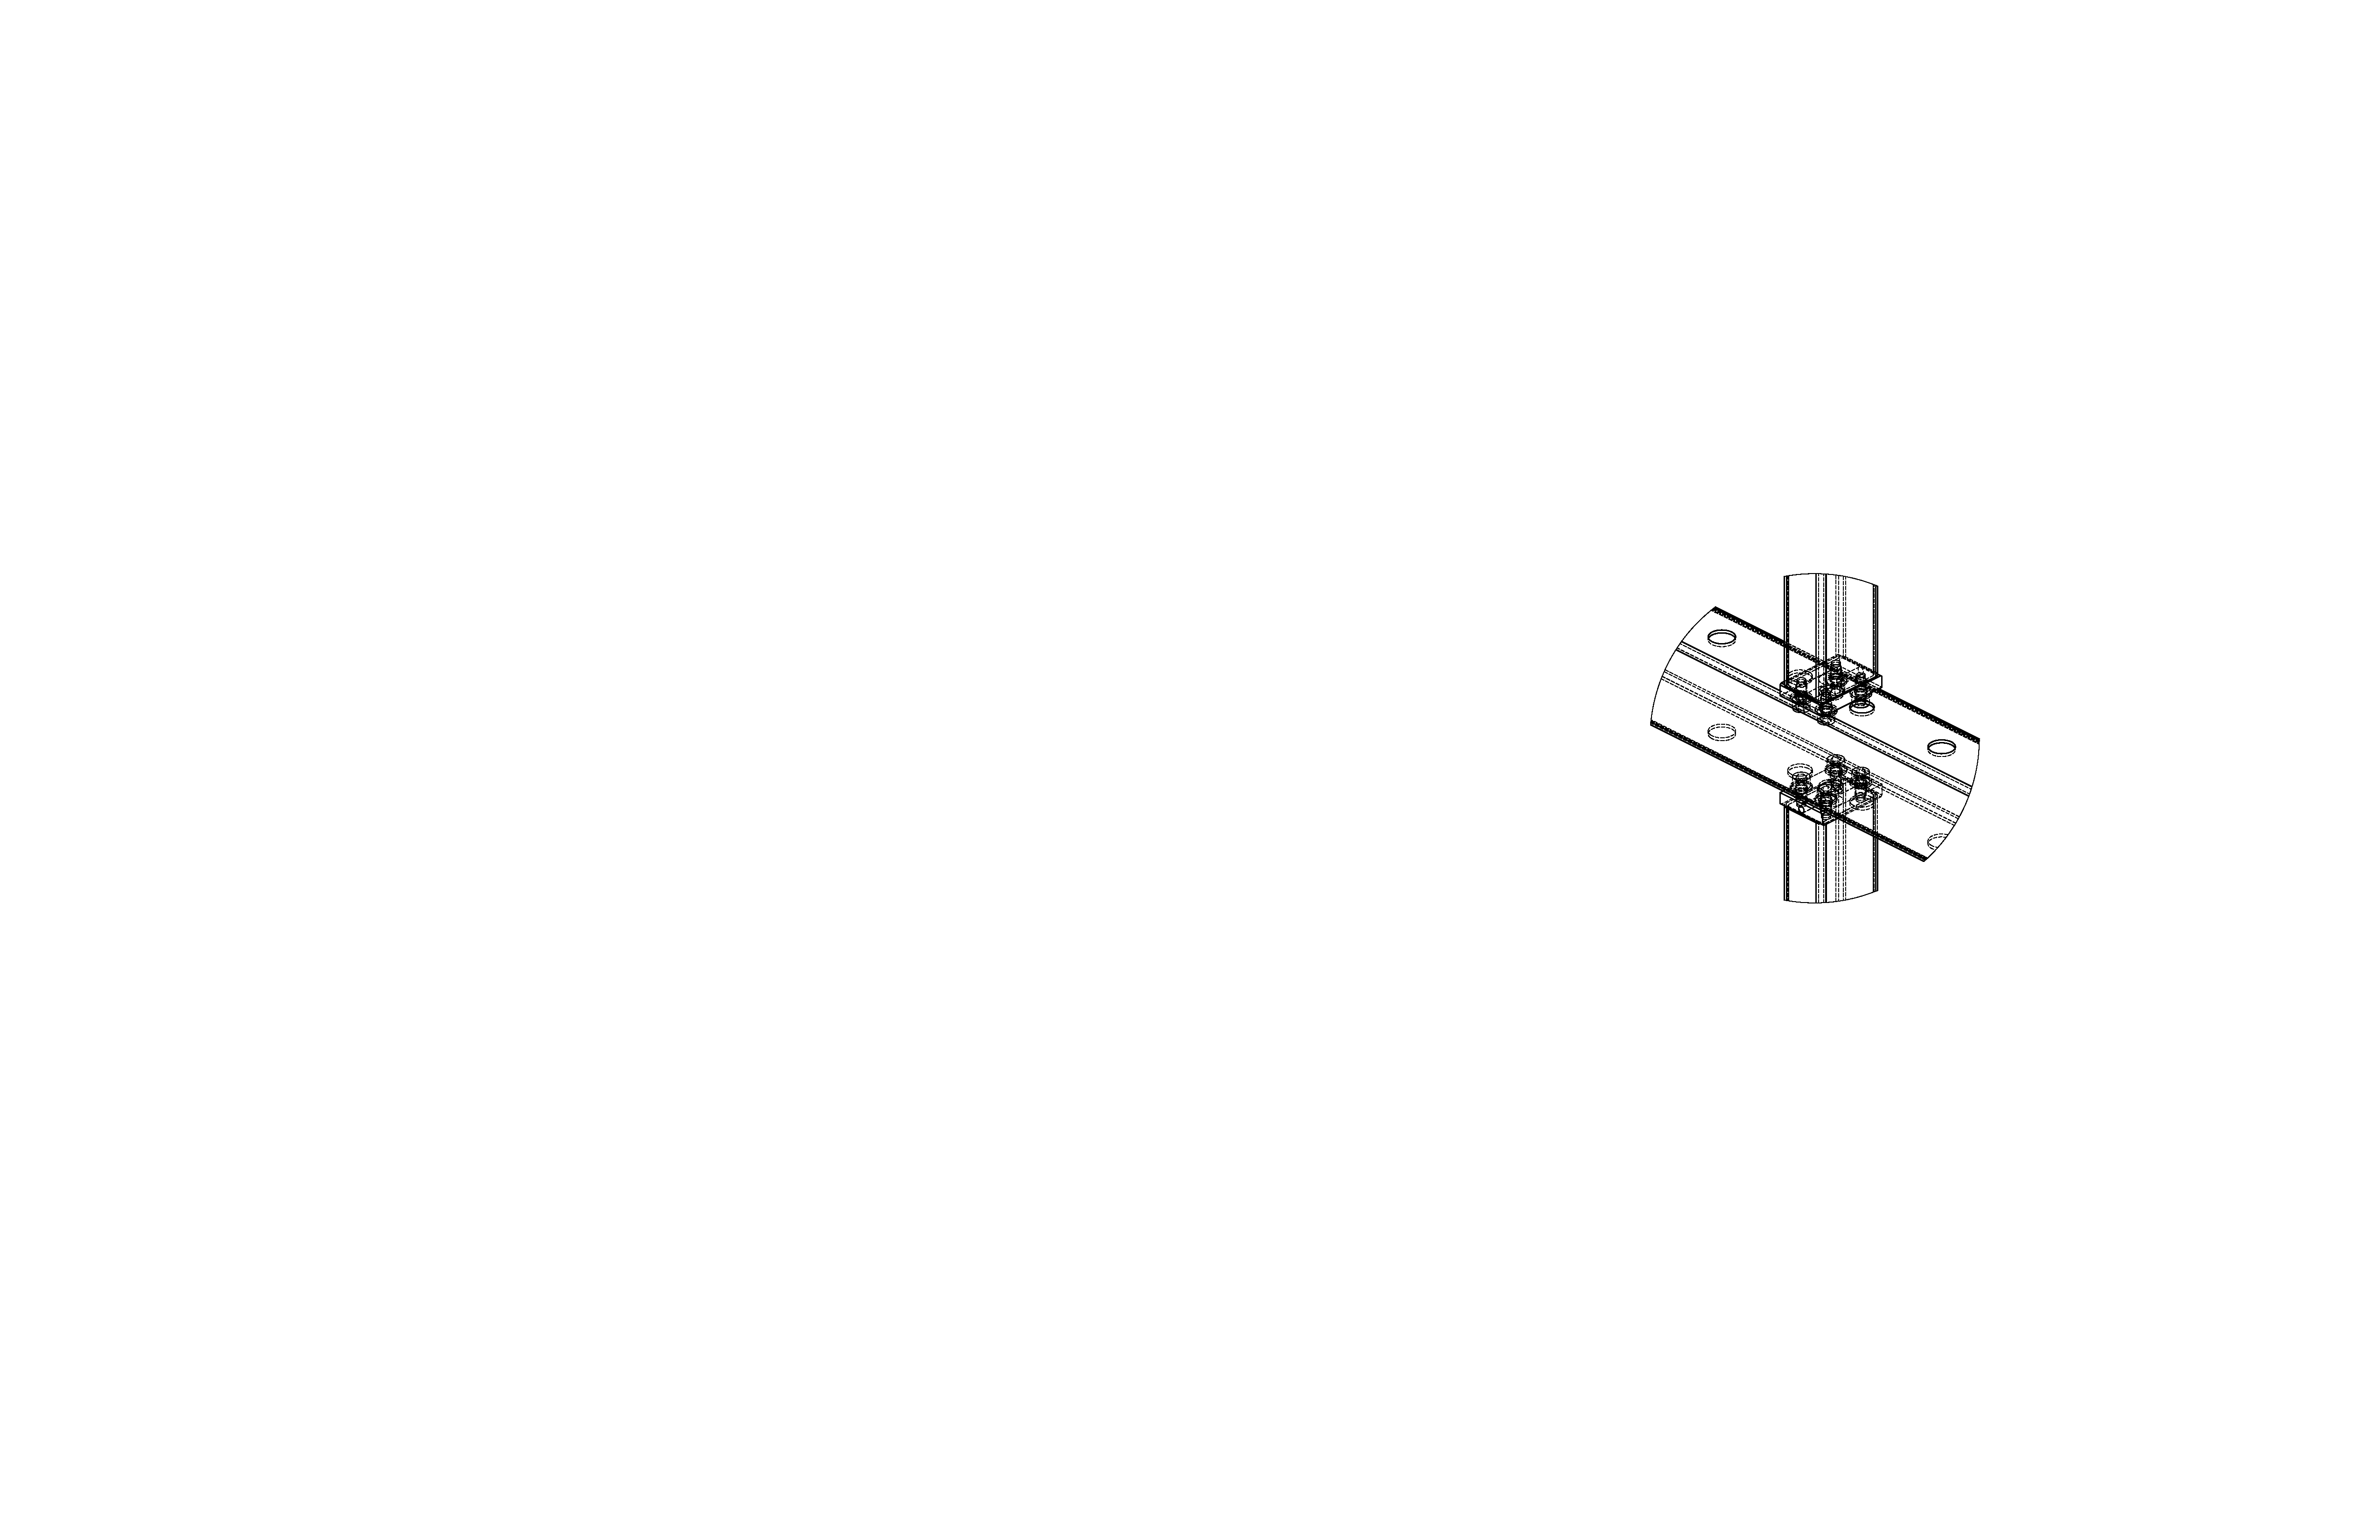
\includegraphics[width=0.45\textwidth]{sp-apa-joint-detail-2.pdf} 
%\end{dunefigure}

The \dword{apa} frames also house the \dword{pds}.  %In the \dword{pdsp} design, 
Rectangular slots are machined in the outer frame tubes and guide rails are used to slide in \dword{pd} elements from the edges. %although alternative \dword{pd} designs are being considered for the \dwords{spmod}. %DUNE. 
(See Section~\ref{sec:fdsp-apa-intfc} for more details on interfacing with the \dword{pds}.)   

In a \dword{fd} \dword{spmod}, pairs of \dword{apa} frames will be mechanically connected to form a \tpcheight %\SI{12}{m} 
tall structure with electronics for \dword{tpc} readout at both the top and bottom of this two-frame assembly and \dwords{pd} installed throughout.  The \dword{apa} frame design, therefore, must support cable routing to the top of the detector from both the bottom \dword{apa} readout electronics and the \dwords{pd} mounted throughout both \dwords{apa}.  %The dimensions of the stainless steel tube sections used in the frame are currently being revisited from that used in \dword{pdsp} to ensure sufficient space is available to accommodate all detector cables.  
Again, see Section~\ref{sec:fdsp-apa-intfc} on interfaces or Chapter~\ref{ch:fdsp-pd} for more details.
%the Photon Detector Chapter in the \dword{tdr} for more information.

%\fixme{from Nora: I suggest line 116 be rephrased in this way for clarity. The dimensions of the stainless steel tube sections used in the frame may be changed from what was used in \dword{pdsp} to ensure the frame has sufficient space to accommodate all detector cables. }

\forlbnc{Finite Element Analysis has been conducted on the frames, both at room and LAr temperatures, and a structural design review started in March.  A short summary and conclusions will be added here once the review report is available.}

%%%%%%%%%%%%%%%%%%%%%%%%%%%%%%%%%%%%%%%%%%%%%%%%%%%%%%%%%%%%%%%%%%%%%
\subsection{Grounding Mesh}
\label{sec:fdsp-apa-mesh}

Beneath the layers of sense wires, a uniform conducting surface is desired to evenly terminate the \efield and improve the uniformity of field lines around the wire planes. A fine woven mesh that is \num{87}\% optically transparent is used to allow scintillation photons to pass through to the \dwords{pd} mounted inside the frame.  The mesh also shields the \dword{apa} wires from the pick-up of signals from other parts of the \dword{apa} or the \dword{pd} system.  

In the \dword{pdsp} \dwords{apa}, the mesh was installed in four long sheets, along the length of the left- and right-hand halves of each side of the \dword{apa} and epoxied directly to the frame. This approach to mesh installation was found to be slow and cumbersome.  For the \dword{dune} mass production, a modular window-frame design is being developed, where mesh is pre-stretched over smaller sub-frames that can be clipped into each gap between cross beams in the full \dword{apa} frame.   This improves the reliability of the installed mesh (more uniform tension across the mesh) and allows much easier installation on the \dword{apa} frame. The mesh will be from a woven conducting 304 stainless steel \SI{80}{\um} wire and is 85\% transparent. The mesh is mounted on 304 stainless steel \SI{20}{mm}$\times$\SI{10}{mm} box section frames. The mesh is stretched over the frame with purpose built jigs and pneumatic actuators then TIG welded around the top surface and again around the side surfaces. There are five different panel designs to match the openings in the APA frames: two for the foot end, two for the head end, and the central panels are all the same. There are 20 panels per \dword{apa}. Stainless steel brackets will be fixed to the inner window sections of the \dword{apa} frame and the panels will be secured into position using steel fasteners. The design ensures that there is good electrical contact between the mesh and the frame. A full-scale \dword{apa} (\dword{apa}-07) has been built at Daresbury Lab for \dword{ce} testing at \dword{cern}, and uses the mesh panel design. Figure~\ref{fig:tpc-apa-mesh} shows images of the new mesh design and the prototypes built for \dword{apa}-07.

\begin{dunefigure}[Photos of APA grounding mesh]{fig:tpc-apa-mesh}
{\dword{apa} grounding mesh construction and installation. a) The mesh panel stretching jig, b) mesh being welded to the support frame, c) model showing the mesh sub-frame (in dark gray) fitting into the \dword{apa} frame (green), and d) photo of an installed mesh panel in \dword{apa}-07.}
\mbox{a) 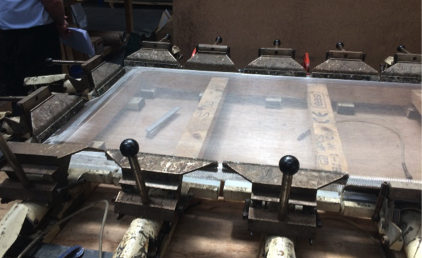
\includegraphics[height=0.23\textheight]{sp-apa-mesh-jig.png} \hspace{0.0mm}
b) 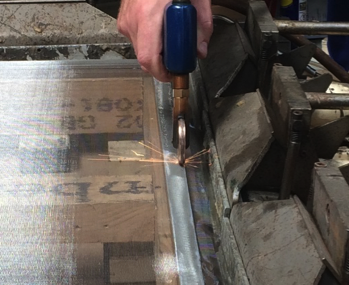
\includegraphics[height=0.23\textheight]{sp-apa-mesh-weld.png}} \\
\vspace{3mm}
\hspace{0.4mm}
\mbox{c) 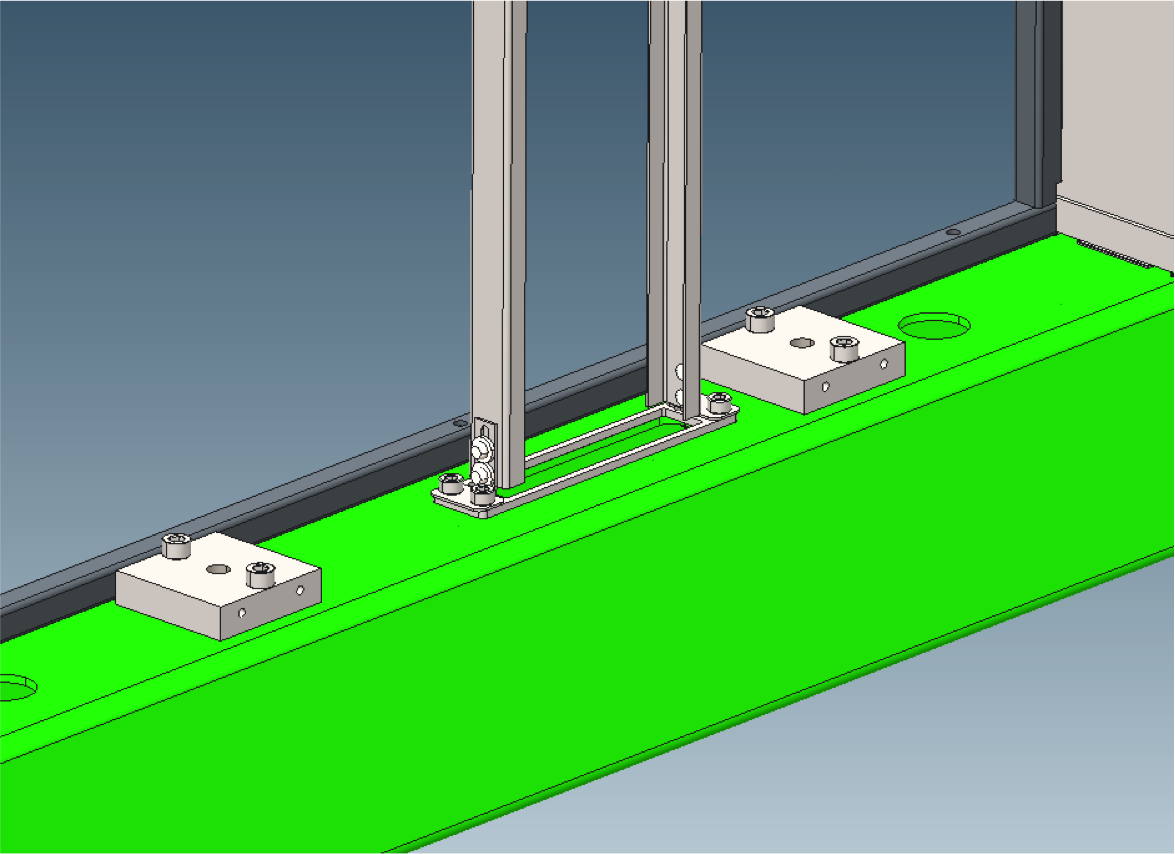
\includegraphics[height=0.23\textheight]{sp-apa-mesh-install-design.png}
d) 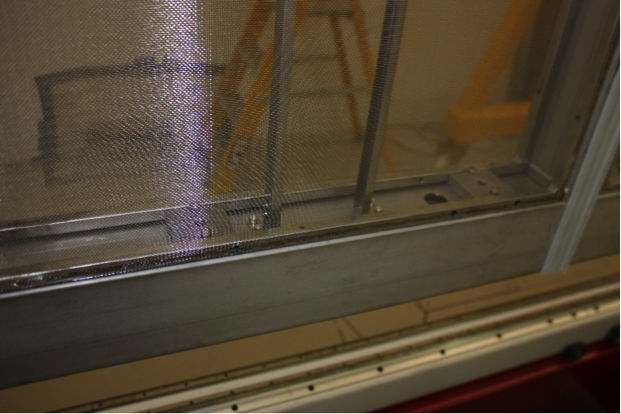
\includegraphics[height=0.23\textheight]{sp-apa-mesh-installed.png}}
\end{dunefigure}

%The mesh was clamped around the perimeter of the opening and then pulled tight (by opening and closing clamps, as needed, during the process).  Once the mesh was taut, a \SI{25}{mm} wide strip was masked off around the opening, and epoxy was applied through the mesh to attach it directly to the steel frame.  Although measurements showed that this gives good electrical contact between the mesh and the frame, a deliberate electrical connection was also made.   dFigure~\ref{fig:tpc-apa-mesh-application}epicts the mesh application setup for a full-size \dword{pdsp} \dword{apa}.
\begin{comment}
\begin{dunefigure}[Photos of APA grounding mesh application in ProtoDUNE-SP]{fig:tpc-apa-mesh-application}
{Grounding mesh being clamped to the \dword{apa} and taped off, ready for gluing to a \dword{pdsp} frame.}
%\setlength{\fboxsep}{0pt}
%\setlength{\fboxrule}{0.5pt}
%\fbox{\includegraphics[height=0.6\textwidth]{apa-mesh-application.png}
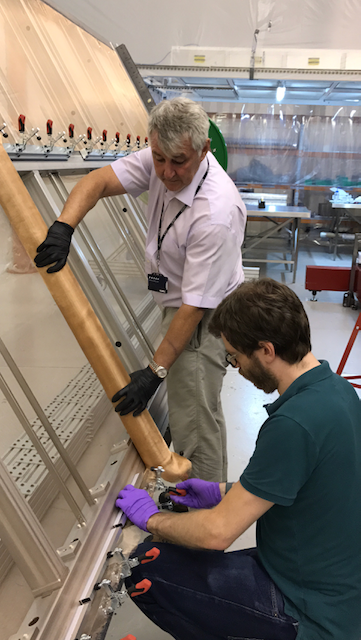
\includegraphics[height=0.6\textwidth]{sp-apa-mesh-application.png} \quad
%} \quad
%\fbox{\includegraphics[height=0.6\textwidth]{apa-mesh-applied.jpg}
%}
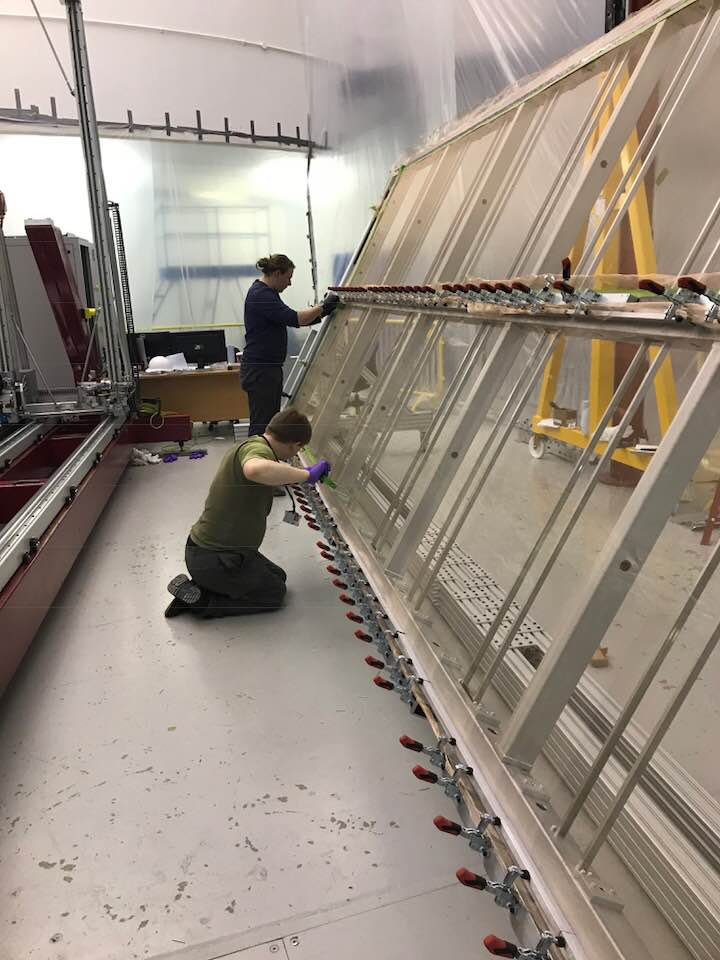
\includegraphics[height=0.6\textwidth]{sp-apa-mesh-applied.jpg}
\end{dunefigure}
%\fixme{Replacing ProtoDUNE-SP in the caption with the dword generated an error. Don't know why. Anne}
\end{comment}
%Installing the mesh as described is difficult; the mesh is prone to wrinkling, %being left 
%which can affect the \efield uniformity and the transparency of the wire planes. For the DUNE mass production, a window-frame design is being considered, where mesh is pre-stretched over smaller sub-frames that can be clipped into each gap between cross beams in the full \dword{apa} frame.  See Section~\ref{sec:fdsp-apa-prod} for more information.


%%%%%%%%%%%%%%%%%%%%%%%%%%%%%%%%%%%%%%%%%%%%%%%%%%%%%%%%
\subsection{Wires}
\label{sec:fdsp-apa-wires}

The \SI{152}{$\mu$m} (\SI{.006}{in}) diameter beryllium copper (CuBe) wire chosen for use in the \dword{apa}s is known for its high durability and yield strength. It is composed of \num{98}\,\% copper, \num{1.9}\,\% beryllium, and a negligible amount of other elements. Each \dword{apa} contains a total of \SI{23.4}{km} of wire.  

The key properties for its use in the \dword{apa}s are low resistivity, high tensile or yield strength, and a coefficient of thermal expansion suitable for use with the \dword{apa}'s stainless steel frame (see Table~\ref{tab:wire} for a summary of properties).  Tensile strength of the wire describes the wire-breaking stress.  The yield strength is the stress at which the wire starts to take a permanent (inelastic) deformation and is the important limit for this case. The wire purchased from Little Falls Alloys~\footnote{Little Falls Alloys\texttrademark, \url{http://www.lfa-wire.com/}} for use on \dword{pdsp} had tensile strength higher than \SI{1380}{MPa} and yield strength more than \SI{1100}{MPa} (\SI{19.4}{N} for \SI{152}{$\mu$m} diameter wire).  The stress while in use is around \SI{280}{MPa} (\SI{5}{N}), leaving a comfortable margin.

The coefficient of thermal expansion (CTE) describes how a material expands or contracts with changes in temperature.  The CTEs of CuBe alloy and \num{304} stainless steel are very similar.  Integrated down to \SI{87}{K}, they are \SI{2.7}{mm/m} for stainless steel and \SI{2.9}{mm/m} for CuBe. The wire contracts slightly more than the frame, so for a wire starting at \SI{5}{N} at room temperature, for example, the tension increases to around \SI{5.5}{N} when everything reaches \lar temperature.  

The change in wire tension during \cooldown is also important.  In the worst case, the wire cools quickly to \SI{87}{K} before any significant cooling of the much larger frame.  In the limiting case with complete contraction of the wire and none in the frame, the tension would peak around \SI{11.7}{N}, which is still well under the \SI{20}{N} yield tension. In practice, however, the cooling will be done gradually to avoid this tension spike as well as other thermal shocks to the detectors.

\begin{dunetable}[Beryllium copper (CuBe) wire properties]{lr}{tab:wire}{Summary of properties of the beryllium copper wire used on the \dword{apa}s.}
Parameter & Value \\ \toprowrule
Resistivity & 7.68 $\mu\Omega$-cm $@$ 20$^{\circ}$ C \\ \colhline
Resistance & 4.4 $\Omega$/m $@$ 20$^{\circ}$ C \\ \colhline
Tensile strength (from property sheets)  & \SI{1436}{MPa} / \SI{25.8}{N} for \SI{152}{$\mu$m} wire \\ \colhline
%Tensile strength (from actual wire)  & \SI{212530}{psi} / \SI{26.4}{N} for \SI{152}{$\mu$m} wire \\ \colhline
CTE of beryllium copper integrated to \SI{87}{K}  & \SI{2.9e-3}{m/m} \\ \colhline
CTE of stainless steel integrated to \SI{87}{K}  & \SI{2.7e-3}{m/m} \\
\end{dunetable}


%%%%%%%%%%%%%%%%%%%%%%%%%%%%%%%%%%%%%%%%%%%%%%%%%%%%%%%%%%%%%%%%
\subsection{Wire Boards and Anchoring Elements}
\label{sec:fdsp-apa-boards}

To guide and secure the \num{3520} wires on an \dword{apa}, stacks of custom FR4 circuit boards attach to the outside edges of the frame, as shown in the engineering drawings in Figure~\ref{fig:apa-wire-boards}.  There are \num{337} total circuit boards on each \dword{apa} (\num{50550} in \num{150} \dword{apa}s), where this number includes 204 wire boards, 72 cover boards, 20 \dword{cr} boards, 20 $G$-layer bias boards, 20 \dword{ce} adapter boards, and one \dword{shv} board to distribute bias voltages to the planes.

\begin{dunefigure}[Wire carrier board layout on the APA frames]{fig:apa-wire-boards}
{Engineering drawings that illustrate the layering of the wire carrier boards that are secured along the perimeter of the \dword{apa} steel frames. Left: The full set of $V$-layer boards.  Right: Detail showing the full stack of four boards at the head end of the \dword{apa}.}
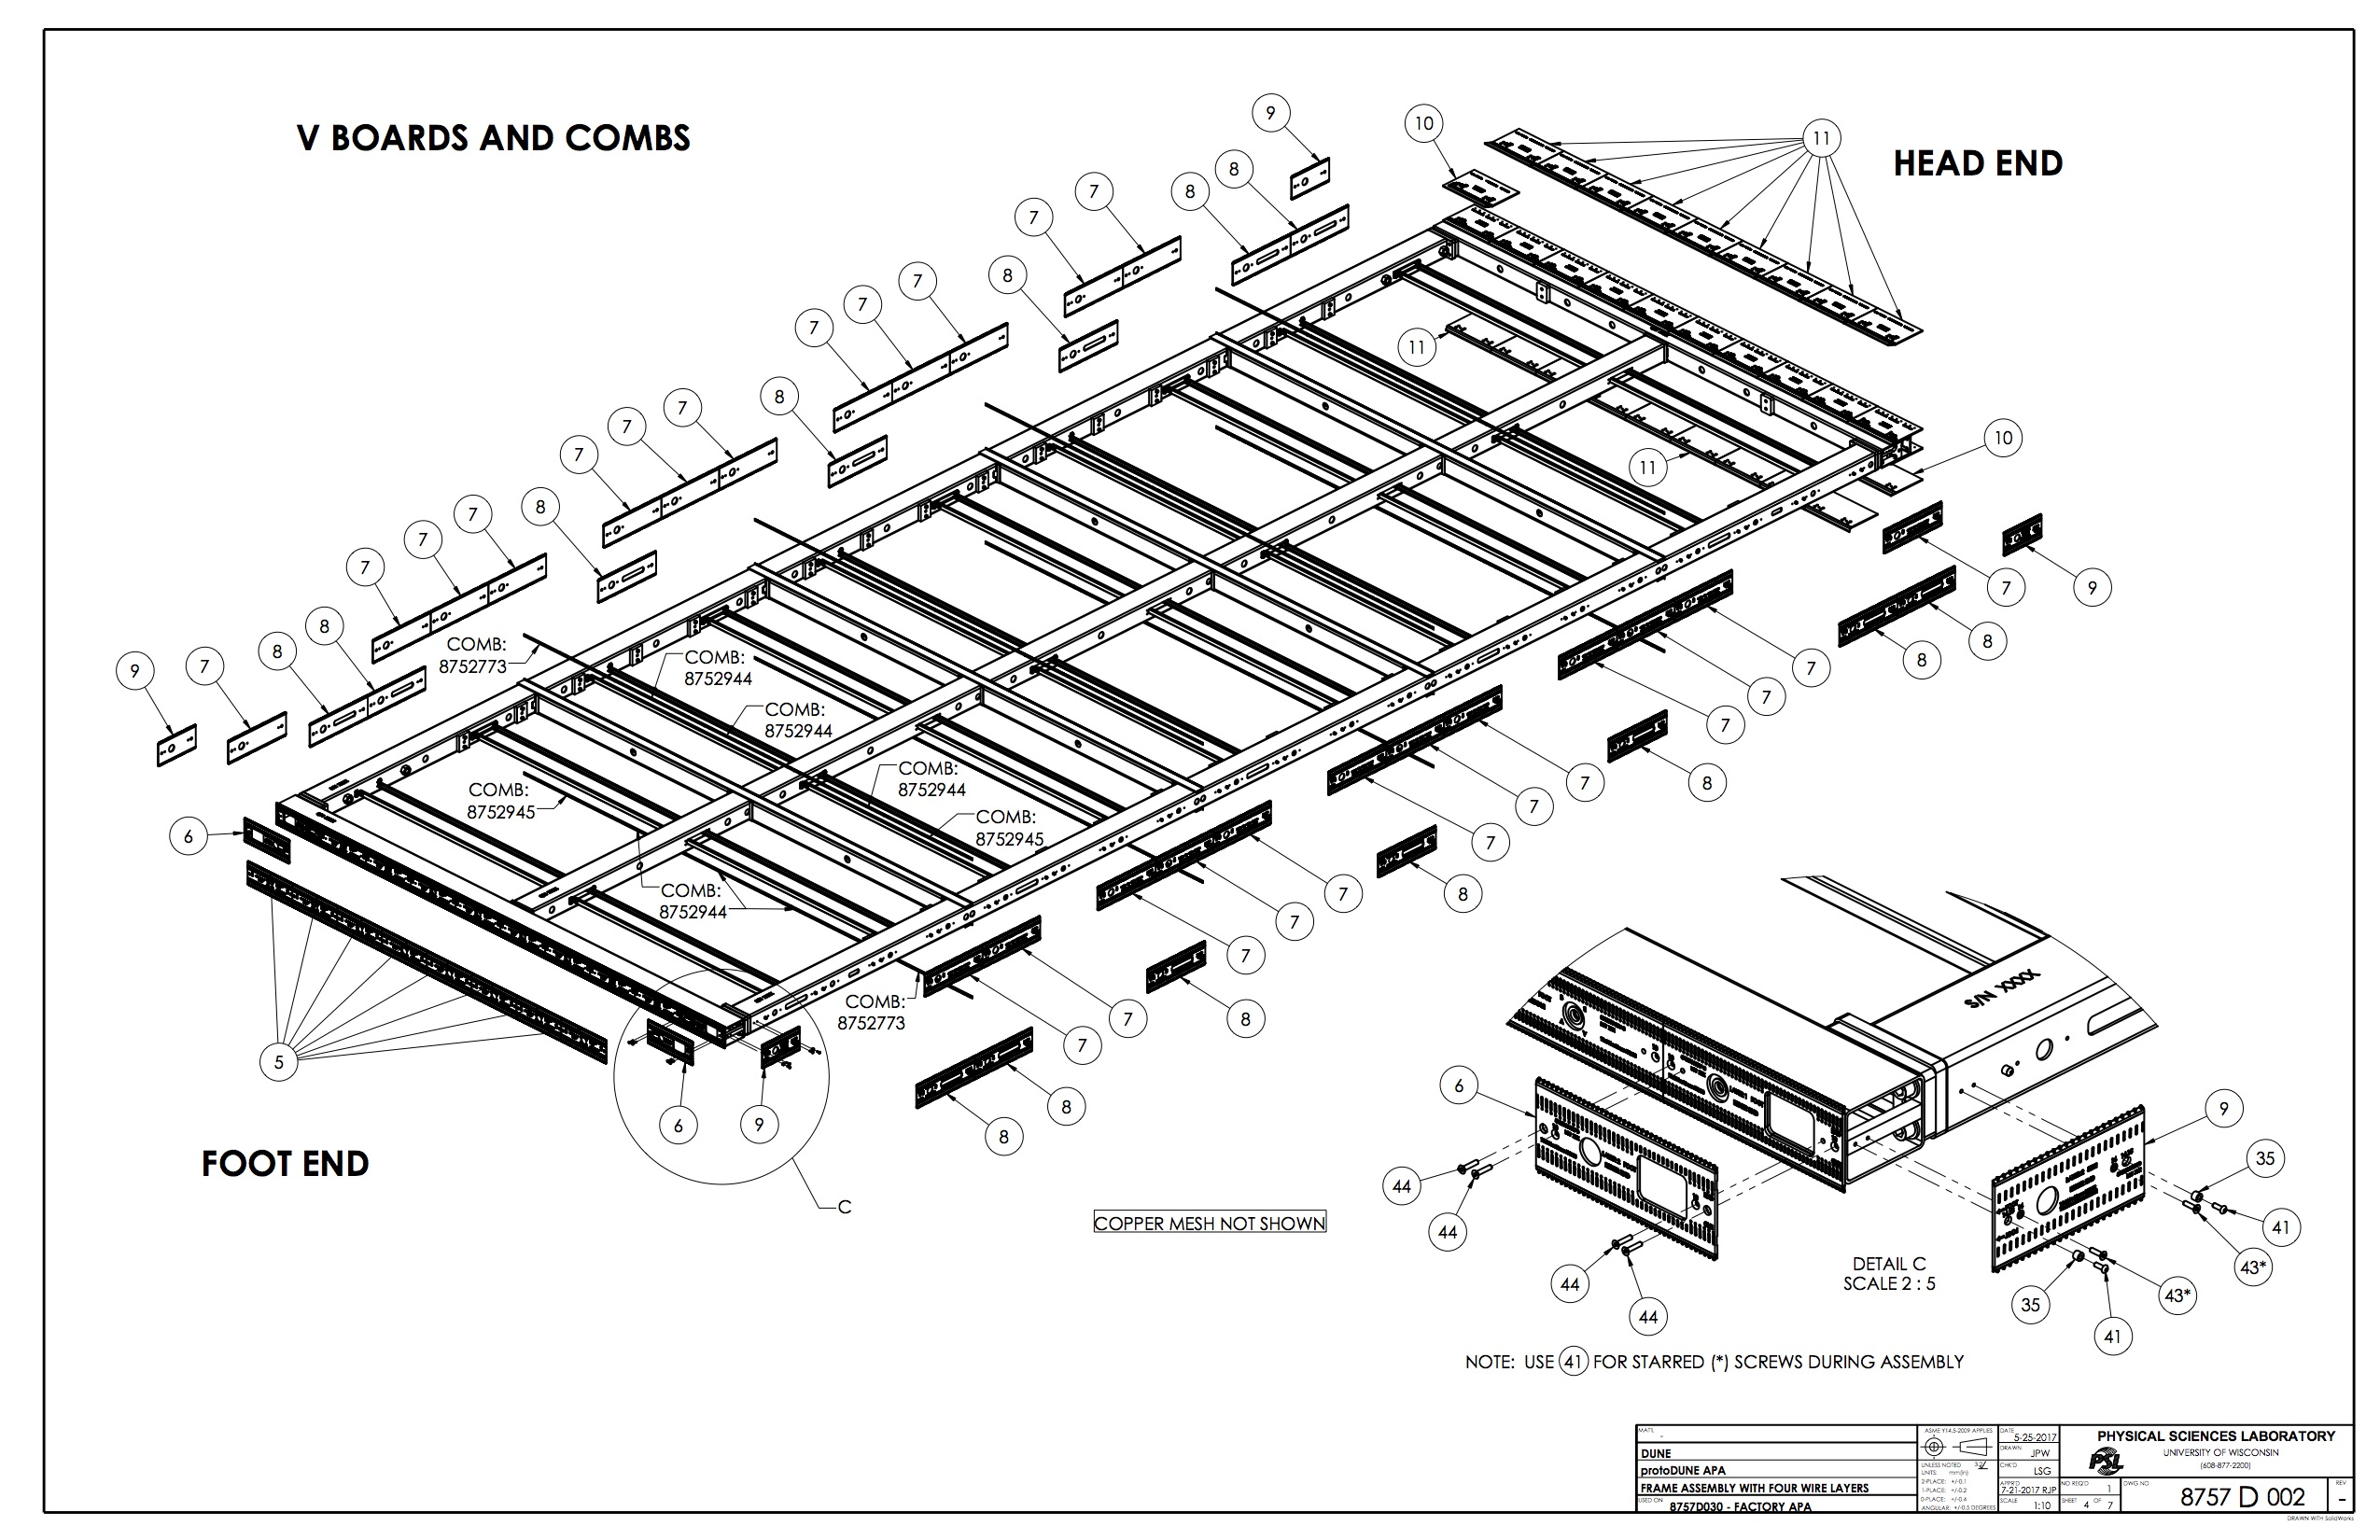
\includegraphics[width=0.48\textwidth]{sp-apa-drawing-v-boards-exploded.jpg}
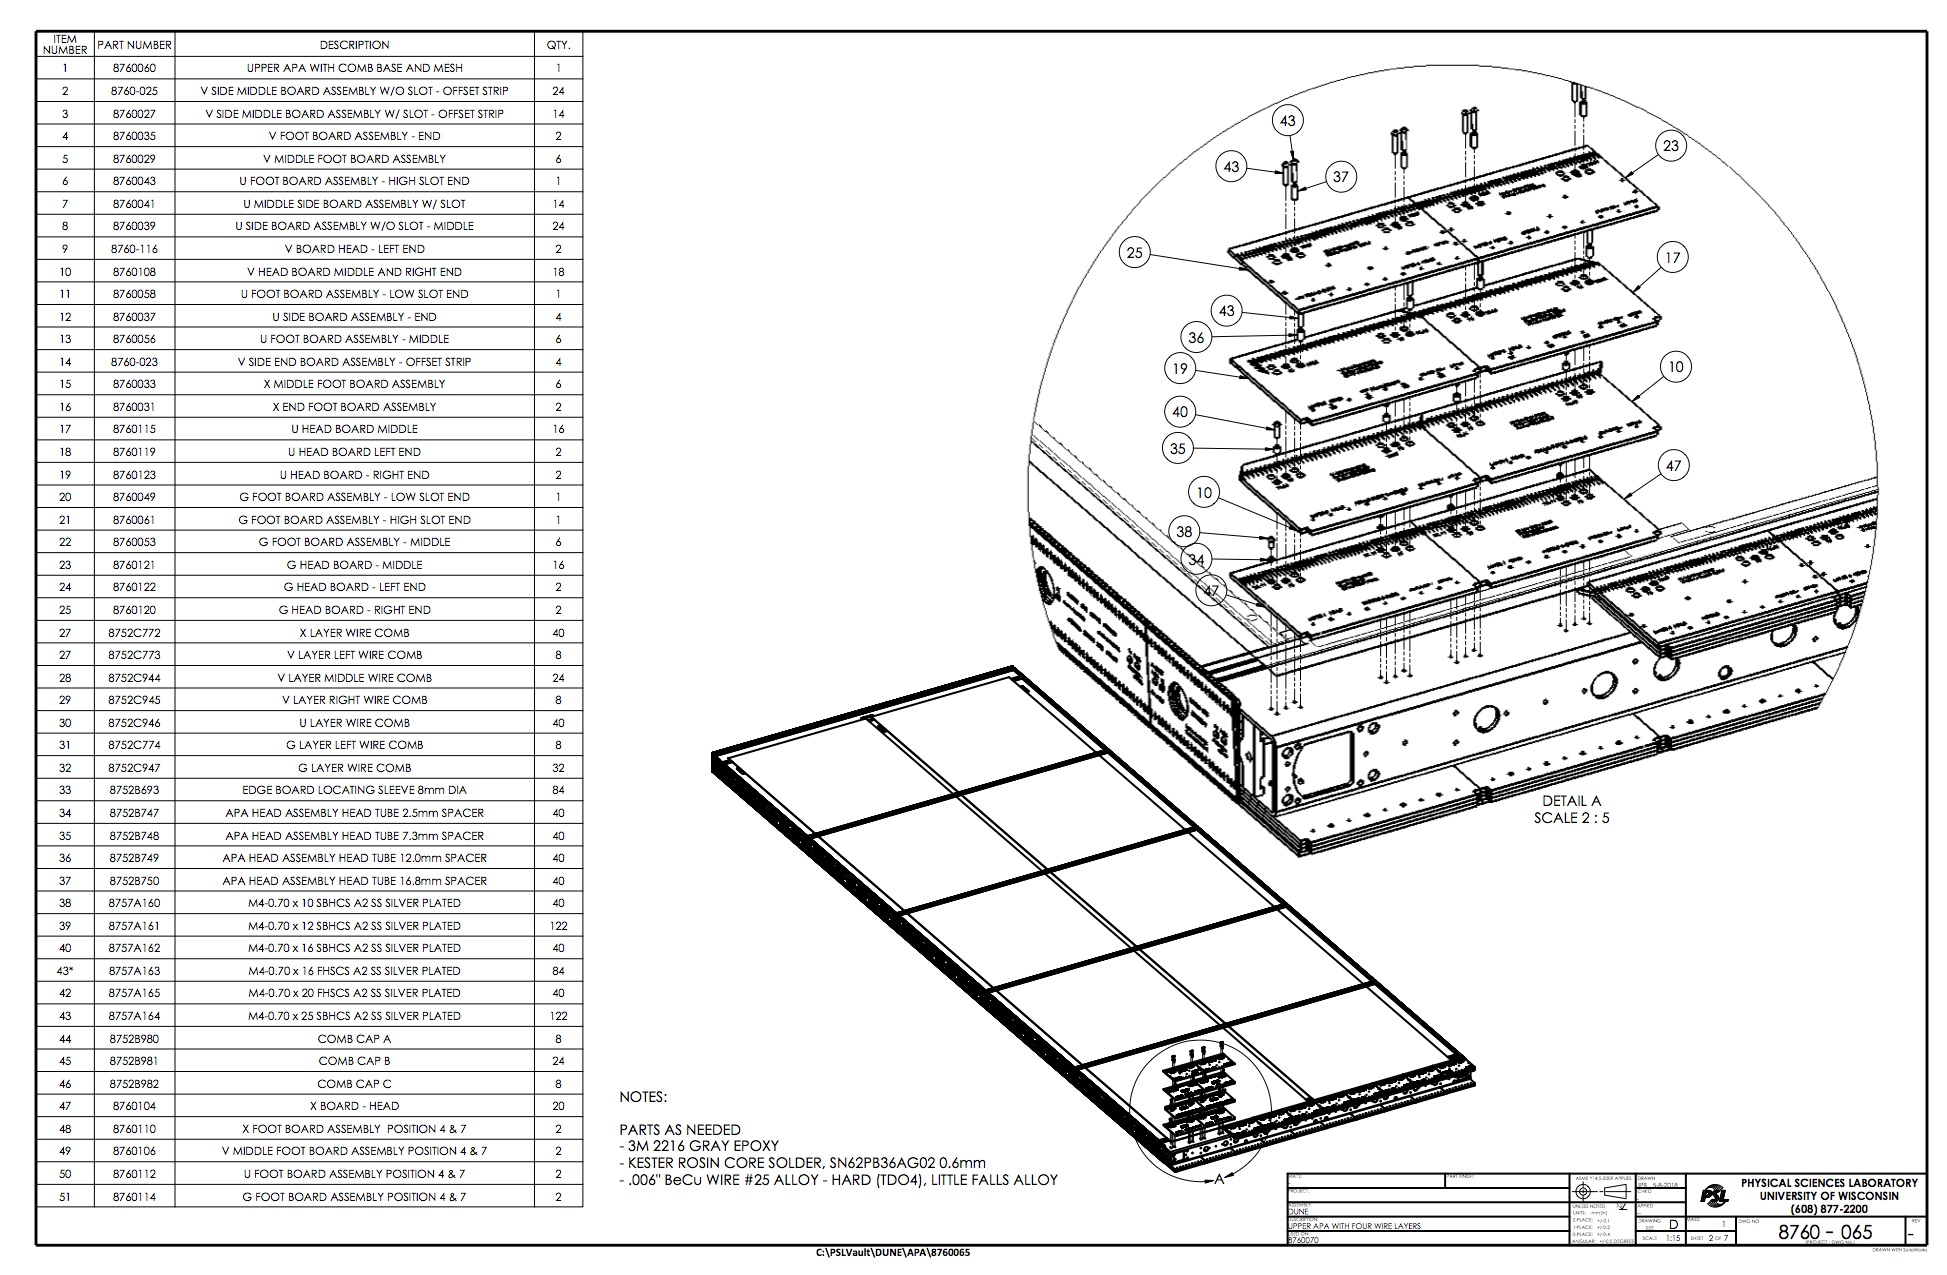
\includegraphics[width=0.48\textwidth]{sp-apa-drawing-board-stack-detail.jpg}
\end{dunefigure}


%%%%%%%%%%%%%%%%%%%%%%%%%%%%%%%%%%%%%%%
\subsubsection{Head Electronics Boards}

All \dword{apa} wires terminate on wire boards stacked along the electronics end of the \dword{apa} frame.  The board stack at the head end is shown in Figure~\ref{fig:apa-wire-boards}. Attaching the wire boards begins with the $X$-plane (lowest). Once the $X$-plane wires are strung on both sides of the \dword{apa} frame, they are soldered and epoxied to their wire boards and trimmed. Next, the $V$-plane boards are epoxied in place and the $V$ wires installed, followed by the $U$-plane boards and wires and finally the $G$-plane boards and wires. The wire plane spacing of \planespace %\SI{4.75}{mm} 
is set by the thickness of these wire boards.   

Mill-Max\footnote{Mill-Max\texttrademark{}, \url{https://www.mill-max.com/}} pins and sockets provide electrical connections between circuit boards within a stack. They are pressed into the circuit boards and are not repairable if damaged. To minimize the possibility of damaged pins, the boards are designed so that the first wire board attached to the frame has only sockets. All boards attached subsequently contain pins that plug into previously mounted boards. This process eliminates exposure of any pins to possible damage during winding, soldering, or trimming.

The $X$, $U$ and $V$ layers of wires are connected to the \dword{ce} (housed in boxes mounted on the \dword{apa}) either directly or through DC-blocking capacitors.  Ten stacks of wire boards are installed across the width of each side along the head of the \dword{apa}.  The $X$-layer board in each stack has room for \num{48} wires, the $V$-layer has 40 wires, the $U$-layer \num{40} wires, and the $G$-layer \num{48} wires.  Each board stack, therefore, has \num{176} wires but only \num{128} signal channels since the $G$ wires are not read out. With a total of \num{20} stacks per \dword{apa}, this results in \num{2560} signal channels per \dword{apa} and a total of \num{3520} wires starting at the top of the \dword{apa} and ending at the bottom. Many of the capacitors and resistors that in principle could be on these wire boards are instead placed on the attached CR boards (see next section) to improve their accessibility in case of component failure. Figure~\ref{fig:tpc_apa_electronics_connectiondiagram} depicts the connections between the different elements of the \dword{apa} electrical circuit at the head end of the frame. 

\begin{dunefigure}[APA wire board connection to electronics]{fig:tpc_apa_electronics_connectiondiagram}{The wire board stack at the head end of an \dword{apa} and the connection to the \dword{ce}. The set of wire boards within a stack can be seen on both sides of the \dword{apa}, with the \dword{cr} board extending further to the right to provide a connection to the \dword{ce}.}
%\setlength{\fboxsep}{0pt}
%\setlength{\fboxrule}{0.5pt}
%%\includegraphics[width=0.62\textwidth, trim=0mm 0mm 5mm 0mm, clip]{apa-board-connections.png}
%\fbox{%\includegraphics[width=0.37\textwidth]{apa-board-stack.png}}
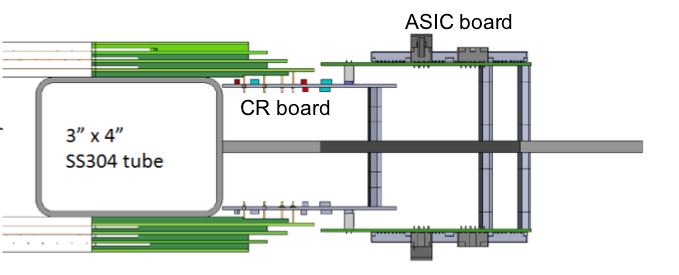
\includegraphics[width=0.60\textwidth, trim=0mm 0mm 5mm 0mm, clip]{sp-apa-board-connections.png}
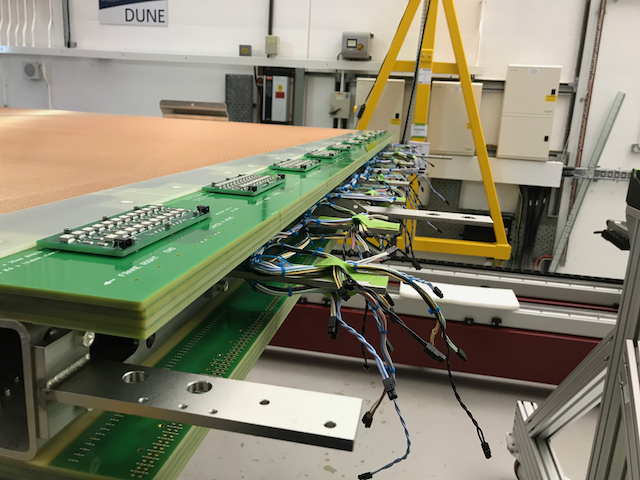
\includegraphics[width=0.35\textwidth]{sp-apa-board-stack.png}
\end{dunefigure} 


%%%%%%%%%%%%%%%%%%%%%%%%%%
\subsubsection{Capacitive-Resistive Boards}
\label{sec:crboards}

The \dword{cr} boards carry a bias resistor and a DC-blocking capacitor for each wire in the $X$ and $U$-planes. These boards are attached to the board stacks after fabrication of all wire planes.   Electrical connections to the board stack are made through Mill-Max pins that plug into the wire boards. Connections from the \dword{cr} boards to the \dword{ce} are made through a pair of \num{96}-pin Samtec\footnote{Samtec\texttrademark \url{https://www.samtec.com/}} connectors.

Surface-mount bias resistors on the \dword{cr} boards have resistance of \SI{50}{\mega\ohm} and are constructed with a thick film on a ceramic substrate. Rated for \SI{2.0}{kV} operation, the resistors measure \num{3.0}$\times$\SI{6.1}{mm^2} (\num{0.12}$\times$\SI{0.24}{in^2}). The selected DC-blocking capacitors have capacitance of \SI{3.9}{nF} and are rated for \SI{2.0}{kV} operation. Measuring %\num{5.6}$\times$\SI{6.4}{mm} (\num{0.22}$\times$\SI{0.25}{in}) across and \SI{2.5}{mm^2} ($\SI{0.10}{in^2}$) 
\SI{5.6 x 6.4}{mm} (\SI{0.22 x 0.25}{in}) across and
\SI{2.5}{mm} (\SI{0.10}{in}) high,  
the capacitors feature flexible terminals to comply with PC board expansion and contraction. They are designed to withstand \num{1000} thermal cycles between the extremes of the operating temperature range. Tolerance is also \num{5}\,\%.

In addition to the bias and DC-blocking capacitors for all $X$ and $U$-plane wires, the \dword{cr} boards include two R-C filters for the bias voltages\footnote{The $V$-plane does not carry a bias voltage, so does not require these components.}. The resistors are of the same type used for wire biasing except with a resistance of \SI{5}{\mega\ohm}, consisting of two \SI{10}{\mega\ohm} resistors connected in parallel. Wire plane bias filter capacitors are \SI{39}{nF}, consisting of ten \SI{3.9}{nF} surface-mount capacitors connected in parallel. They are the same capacitors as those used for DC blocking.

The selected capacitors were designed by the manufacturer to withstand repeated temperature excursions over a wide range. Their mechanically compliant terminal structure accommodates \dword{cte} mismatches. The resistors use a thick-film technology that is also tolerant of wide temperature excursions.  Capacitors and resistors were qualified for \dword{pdsp} by testing samples repeatedly at room temperature and at \num{-190}\,$^\circ$C.  Performance criteria were measured across five thermal cycles, and no measurable changes were observed. During the production of \num{140} \dword{cr} boards, more than \num{10000} units of each component were tested at room temperature, at \dword{lar} temperature, and again at room temperature. No failures or measurable changes in performance were observed.

%%%%%%%%%%%%%%%%%%%%%%%%%%%%%%%%%%%%
\subsubsection{Side and Foot Boards}

The boards along the sides and foot of the \dword{apa} have notches, pins, and other location features to hold wires in the correct position as they wrap around the edge from one side of the \dword{apa} to the other.  

\begin{dunefigure}[Photos of APA side boards showing traces that connect wires around openings]{fig:tpc_apa_sideboardmodel}
{Side boards with traces that connect wires around openings.  The wires are wound straight over the openings, then soldered to pads at the ends of the traces. The wire sections between the pads are then trimmed away.}
%\setlength{\fboxsep}{0pt}
%\setlength{\fboxrule}{0.5pt}
%\fbox{\includegraphics[height=0.28\textheight]{apa-side-board-slot.jpg}
%}\quad
%\fbox{\includegraphics[height=0.28\textheight,trim=0mm 0mm 0mm 25mm,clip]{apa-side-board-round-hole.jpg}
%}
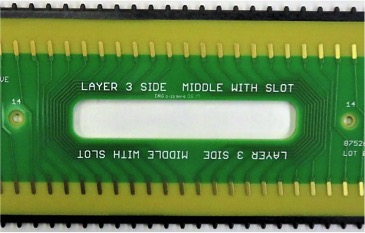
\includegraphics[height=0.28\textheight]{sp-apa-side-board-slot.jpg} \quad
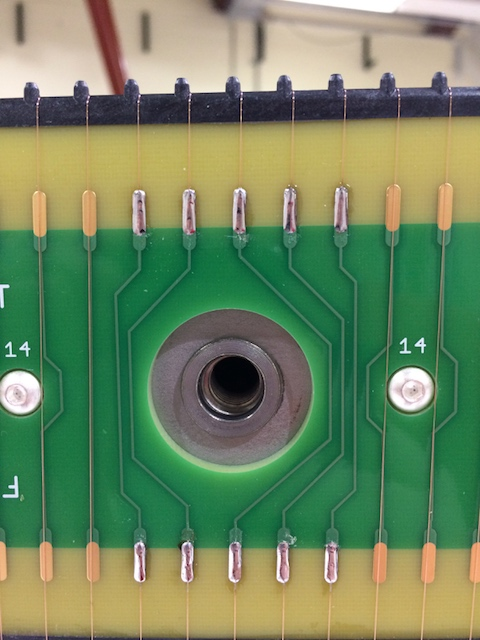
\includegraphics[height=0.28\textheight,trim=0mm 0mm 0mm 25mm,clip]{sp-apa-side-board-round-hole.jpg}
\end{dunefigure}

The edge boards need a number of hole or slot features to provide access to the underlying frame (see Figure~\ref{fig:tpc_apa_sideboardmodel} for examples).  In order that these openings not be covered by wires, the sections of wire that would go over the openings are replaced by traces on the boards.  After the wires are wrapped, the wires over the opening are soldered to pads at the ends of the traces, and the section of wire between the pads is snipped out.  These traces can be easily and economically added to the boards by the many commercial fabricators who make circuit boards. 

The placement of the angled wires are fixed by teeth that are part of an injected molded strip glued to the edge of the FR4 boards.  The polymer used for the strips is Vectra e130i (a trade name for 30$\%$ glass filled liquid crystal polymer, or LCP). It retains its strength at cryogenic temperature and has a CTE similar enough to FR4 that differential contraction is not a problem.  The wires make a partial wrap around the pin as they change direction from the face of the \dword{apa} to the edge.

%%%%%%%%%%%%%%%%%%%%%%%%%%%%%%%%%%%%%%%
\subsubsection{Support Combs}
\label{sec:combs}

Support combs are glued at four points along each side of the \dword{apa}, along the four cross beams. These combs maintain the wire and plane spacing along the length of the \dword{apa}. A dedicated jig is used to install the combs and also provides the alignment and pressure as the glue dries. The glue used is the Gray epoxy \num{2216} described below. Before the jig can be removed and production can continue, an eight-hour cure time is required after comb installation on each side of the \dword{apa}.  Figure~\ref{fig:tpc_apa_sideboardphoto} shows a detail of the wire support combs on a \dword{pdsp} \dword{apa}.

\begin{dunefigure}[Photos of APA side boards on the frame]{fig:tpc_apa_sideboardphoto}
{Left: \dword{apa} corner where end boards meet side boards.  The injection molded teeth that guide the $U$ and $V$ wires around the edge are visible at the bottom. Right: The wire support combs.}
%\setlength{\fboxsep}{0pt}
%\setlength{\fboxrule}{0.5pt}
%\fbox{\includegraphics[height=0.3\textheight]{apa-boards-with-pins.png}
%}\quad
%\fbox{\includegraphics[height=0.3\textheight]{apa-photo-combs.jpg}
%}
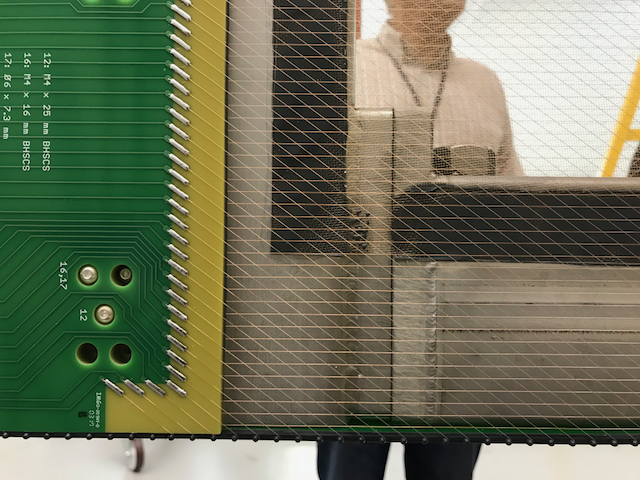
\includegraphics[height=0.32\textheight]{sp-apa-boards-with-pins.png} \quad
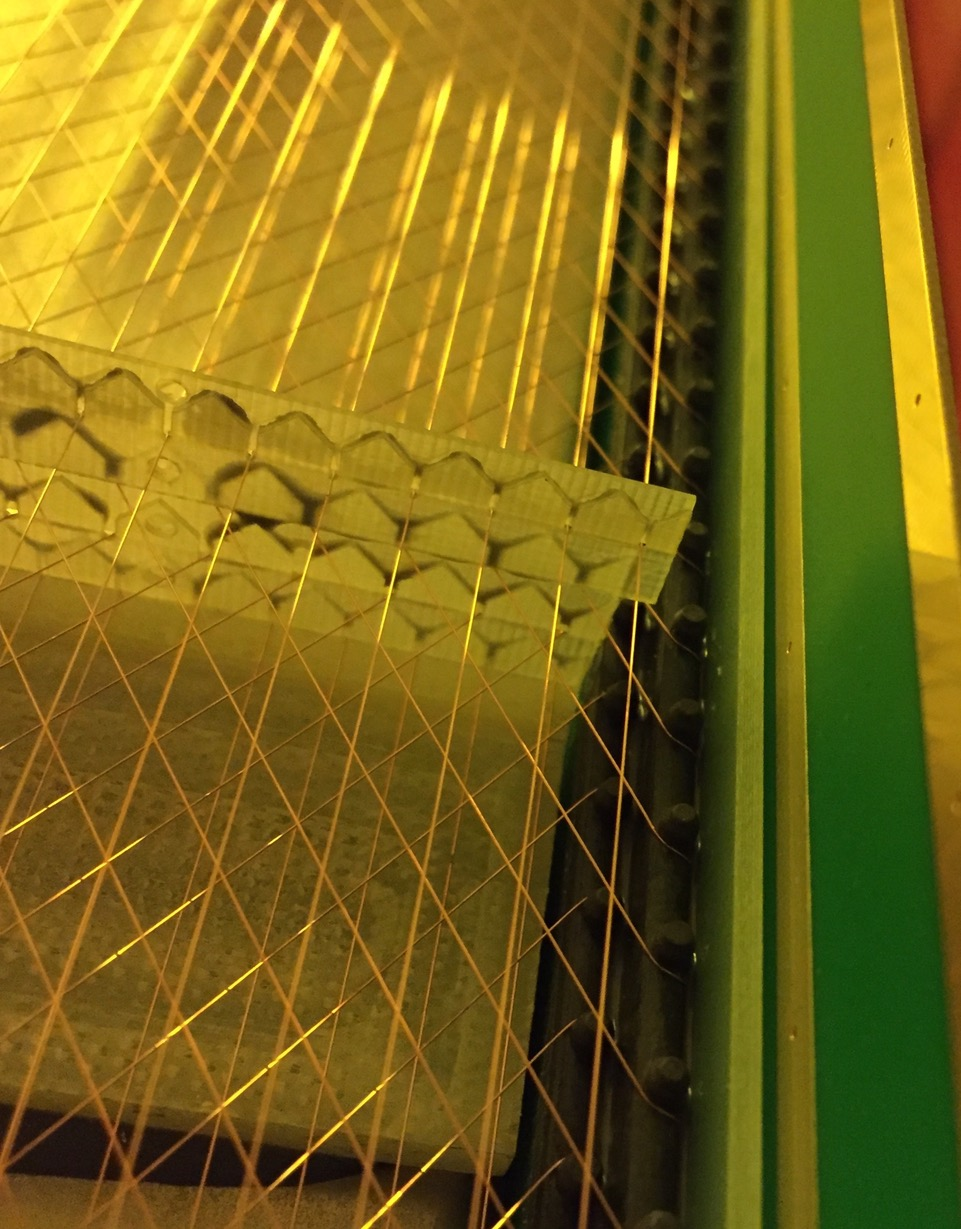
\includegraphics[height=0.32\textheight]{sp-apa-photo-combs.jpg}
\end{dunefigure}

%%%%%%%%%%%%%%%%%%%%%%%%%%%%%%%%%%%%%%%
\subsubsection{Solder and Epoxy}
\label{sec:glue-solder}

The ends of the wires are soldered to pads on the edges of the wire boards.  Solder provides both an electrical connection and a physical anchor to the wire pads. A 62$\%$ tin, 36$\%$ lead, and 2$\%$ silver solder was chosen.  A eutectic mix (63/37) is the best of the straight tin-lead solders, but the 2$\%$ added silver gives better creep resistance.  The solder contains a no-clean flux, and does not need to be removed after soldering. Most of it is encapsulated when subsequent boards are epoxied in place.  At room temperatures and below, the flux is not conductive or corrosive.

Once a wire layer is complete, the next layer of boards is glued on; this glue provides an additional physical anchor. Gray epoxy \num{2216} by 3M\footnote{3M\texttrademark ~\url{https://www.3m.com/}} is used for the glue.  It is strong and widely used (so much data is available), and it retains good properties at cryogenic temperatures.  


%%%%%%%%%%%%%%%%%%%%%%%%%%%%%%%%%
%\subsection{APA-to-APA Connections and Cable Routing}
\subsection{The APA Pair} %Doublet}
\label{sec:fdsp-apa-intfc-apa}

In a \dword{fd} \dword{spmod}, pairs of \SI{6}{m} tall \dword{apa} frames are mechanically connected at their ends to form a \SI{12}{m} tall readout surface.  Figure~\ref{fig:apa-doublet} showed a connected pair (turned on its side).  The \dword{tpc} readout electronics require that the individual \dword{apa} frames must be electrically isolated.   The left panel of Figure~\ref{fig:apa-connections} shows the design for mechanically connecting \dword{apa}s while maintaining electrical isolation.  The two \dword{apa}s are connected through a G10 link that is attached to both frames with a special shoulder screw.  The links connect to the side tubes with a special shoulder screw that screws into plates welded to the frame.  The link pieces are manufactured from G10 to electrically isolate the two frames as required by the \dword{fe} electronics.  

\begin{dunefigure}[Dimensioned diagram of a pair of APAs hanging vertically]{fig:apa-doublet}
{Diagram of an \dword{apa} pair, with connected bottom and top \dword{apa}. The dimensions of the \dword{apa} pair, including the accompanying cold electronics and mechanical supports (the yoke), are indicated.}
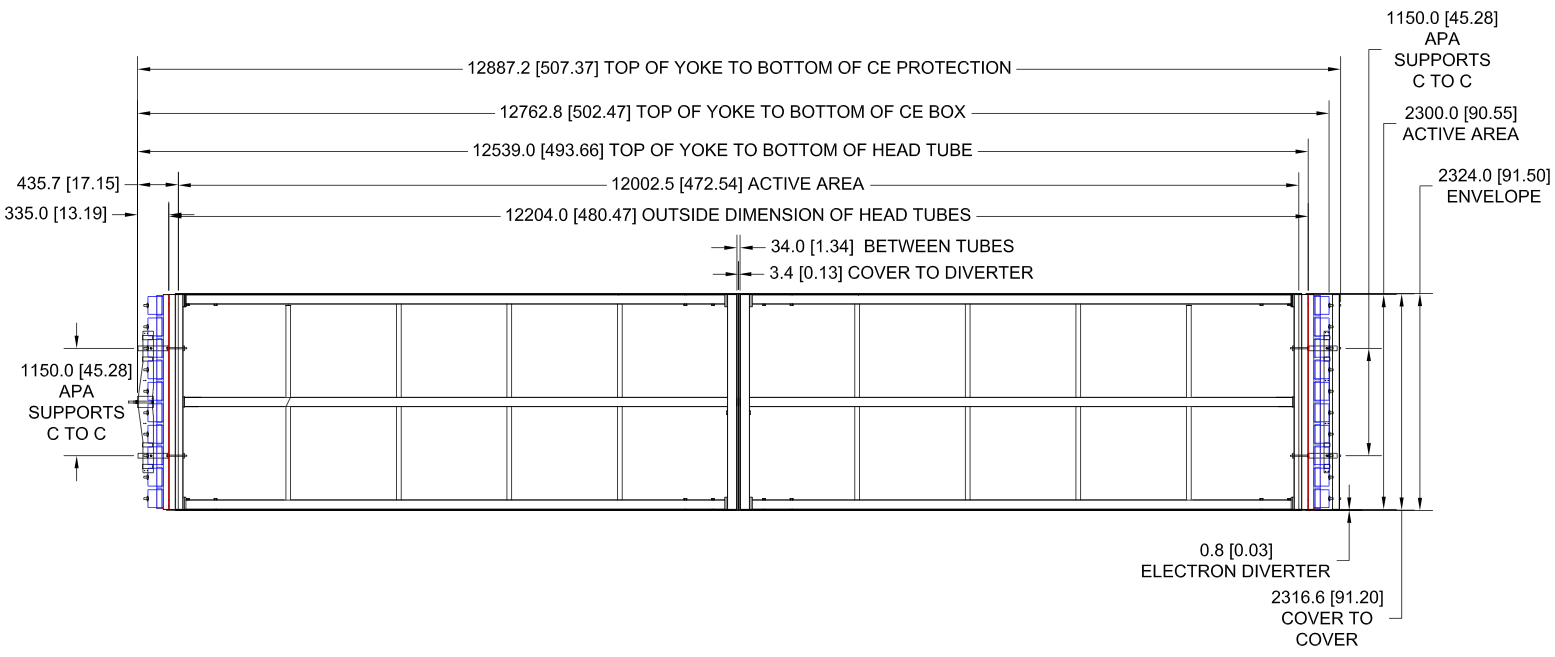
\includegraphics[width=1\textwidth]{sp-apa-stack.jpg} 
\end{dunefigure}

\begin{dunefigure}[APA-to-APA connections]{fig:apa-connections}
{Design for the \dword{apa}-to-\dword{apa} connections.  Left: For the vertical connection there are two G10 links joining the upper \dword{apa} to the lower \dword{apa}; one link connected to one \dword{apa} is shown here.  Right: Along adjoining vertical edges, two pins keep neighboring \dword{apa}s in plane. Two side tubes before engagement with the screw and insulating sleeve installed are shown at the top, and the engaged side tubes are shown below.   }  
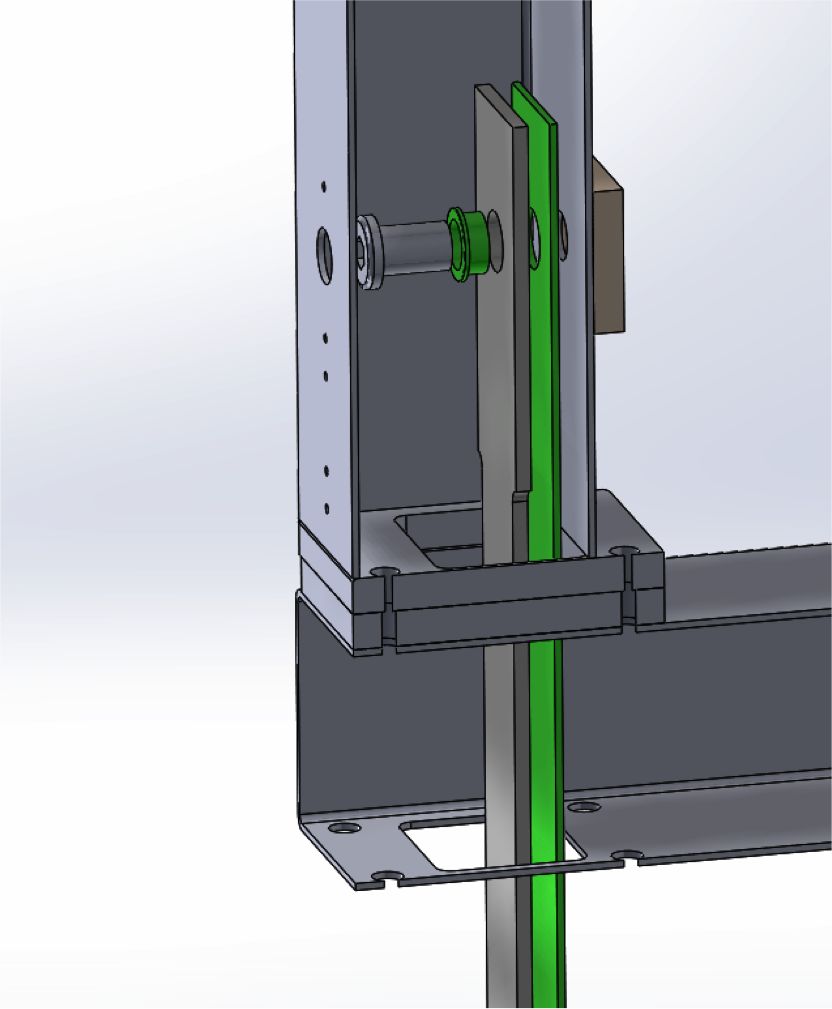
\includegraphics[height=0.32\textheight]{sp-apa-apa-mating.png} \qquad
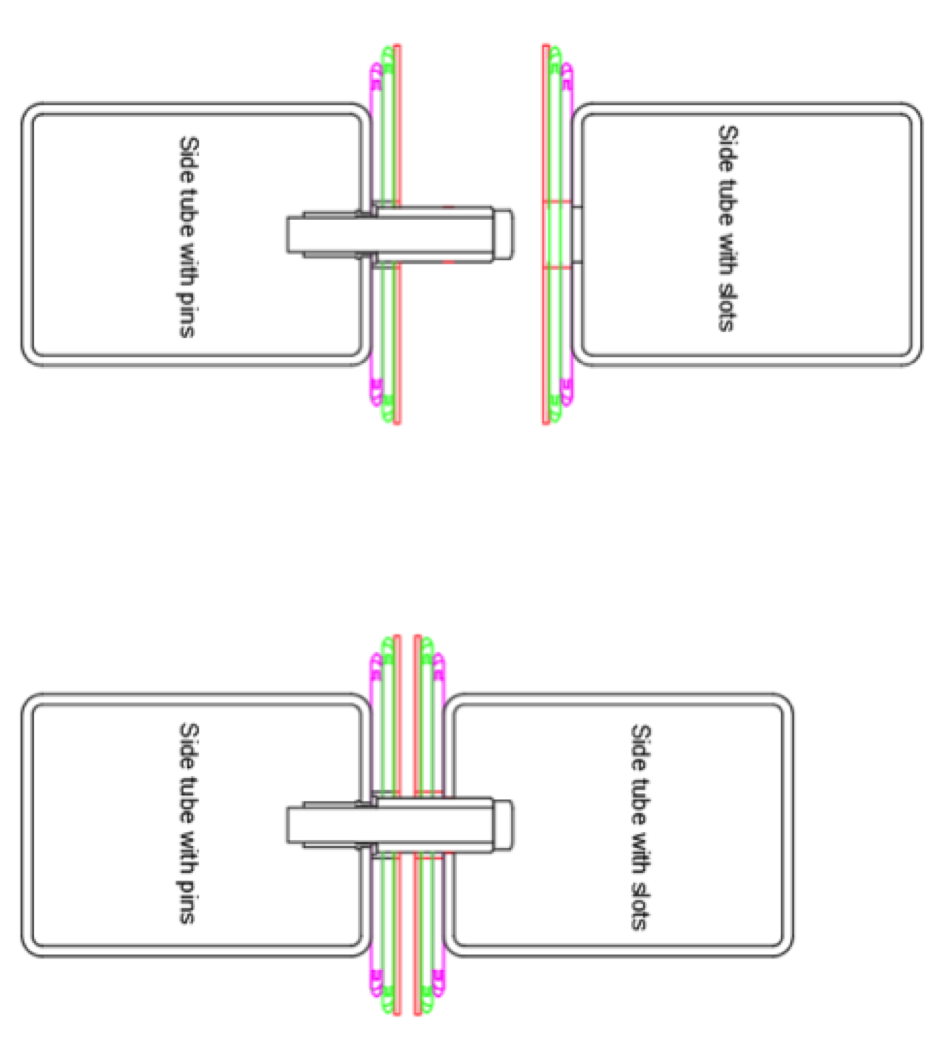
\includegraphics[height=0.32\textheight]{sp-apa-side-mating.png}
\end{dunefigure}

The \dword{apa} yoke, shown in Figure~\ref{fig:apa-yoke}, is a bolted stainless steel structural assembly with a central support point and a pair of pins to connect to the load.  Two tee-shaped brackets referred to as the ``structural tees'' mount to the head tube of the top \dword{apa} and provide the mating pin holes to connect the yoke to the \dword{apa}.  The center support point consists of a M20 stainless steel bolt, oversize washers and a PEEK washer for electrical isolation.   The yoke is mounted to the top \dword{apa} before an \dword{apa} pair %doublet 
is assembled.  To move into the cryostat, the pair %doublet 
is hung from two trolleys that connect to the structural tees. Once in final position the load of the \dword{apa} pair %doublet 
can be transferred from the trolleys to the \dword{dss} in the cryostat through the center support point of the yoke.  To accomplish this, the M20 bolt and washer assembly is inserted from the bottom of the yoke and the threaded end of the bolt connects to the DSS.

\begin{dunefigure}[Yoke that connects an APA pair %doublet 
to the DSS]{fig:apa-yoke} % I got rid of doublet in other chaps
{The yoke at the top of an \dword{apa} pair %doublet 
that provides connection to the \dword{dss}.}
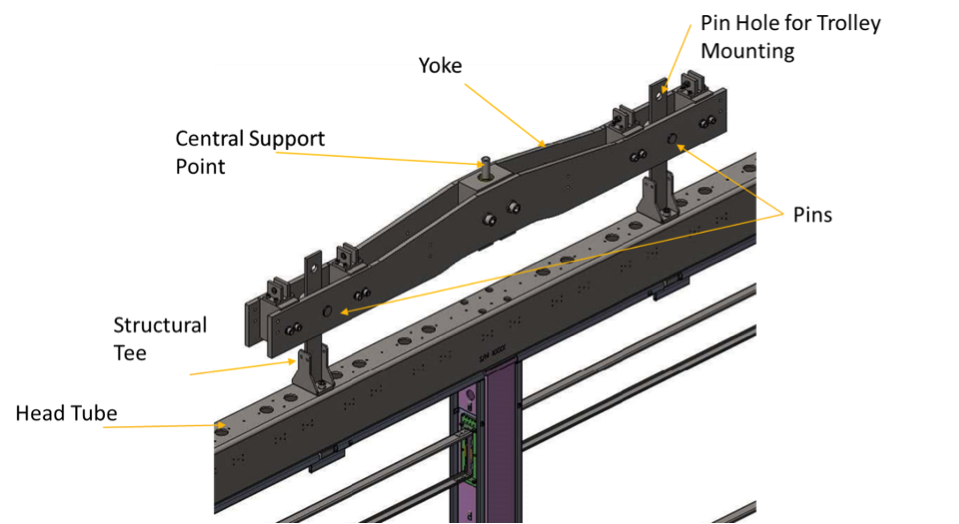
\includegraphics[width=0.95\textwidth]{sp-apa-yoke-labels.png} 
\end{dunefigure}

Adjacent \dword{apa} pairs %doublets 
are kept in plane with each other by simple insertion pins at the top and bottom of the side tubes.  The pins are made up of a screw and an insulating sleeve to ensure electrical isolation, and each pin engages a slot in the adjacent \dword{apa} pair %doublet 
side tubes. The right panel of Figure~\ref{fig:apa-connections} shows a schematic of the side pin connectors before and after insertion.  

Once installed in the detector, a physical gap of \SI{12}{mm} exists along this vertical connection between all adjacent \dword{apa}s at room temperature. Since the \dword{apa}s are suspended under the stainless steel \dword{dss} beams, which contract similarly to that of the \dword{apa} frames, the gaps between most adjacent \dword{apa}s stay about the same (\SI{12}{mm}) in the cold.  The \dword{dss} beams, however, are segmented at \SI{6.4}{m} length, and each beam segment is independently supported by two \dword{dss} feedthroughs, one of which does not allow lateral movement.  As a result, the gaps between \dword{dss} beams open up in the cold by another \SI{17}{mm},  %This additional \SI{17}{mm} needs to be added to the \dword{apa}s spanning the beam boundaries, 
making the physical gaps \SI{29}{mm} as shown in Figure~\ref{fig:sp-apa-gaps}.  The actual gap between the \dword{apa}s' active width, which is defined by the outside faces of the steel frame, is about \SI{16}{mm} wider than the physical gap, so \SI{28}{mm} and \SI{45}{mm}, respectively, in the two scenarios described above.

\begin{dunefigure}[APA-to-APA gaps]{fig:sp-apa-gaps}
{Illustration of the gap width between \dword{apa}s}  
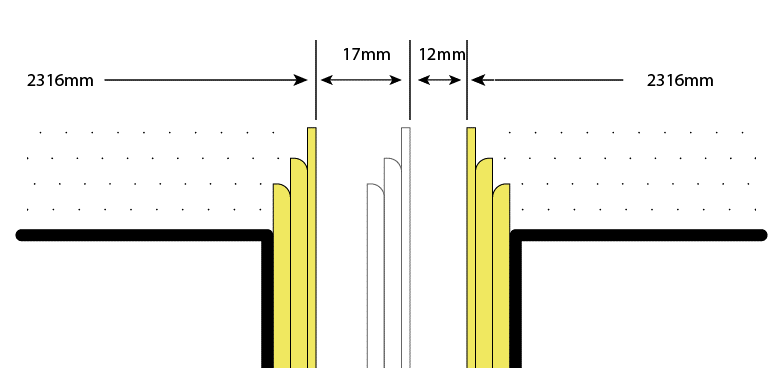
\includegraphics[width=0.8\textwidth]{sp-apa-gaps.png} 
\end{dunefigure}


%Therefore, in the two scenarios described above, the gaps between the active regions are \SI{28}{mm} and \SI{45}{mm}, respectively.  
To minimize the loss of signal charge over the gaps between \dword{apa}s, special electrodes (electron diverters) can be installed along the gaps to nudge the incoming electrons into the active regions of the \dword{apa}s.  Designs are under active consideration, and data from \dword{pd} will play an important role in determining if a diverter system is needed (\dword{pd} had some \dword{apa} gaps with electron diverters installed and some without, enabling comparisons of the tracking and calorimetry performance).  A decision regarding the need for and the design of electron diverters in \dword{dune} is expected by June 2019.

\begin{comment}
are designed to be installed along the gaps to nudge the incoming electrons into the active regions of the \dword{apa}s. The most challenging locations are those across the larger gaps at \dword{dss} beam ends; these gaps only form in the cold.

Figure~\ref{fig:sp-apa-ed-large} shows the design concept for this type of electron diverter.  The thin base plate is mounted over the side cover boards of one \dword{apa} using existing screws holding the cover boards. Along the long edges of the base plate, FRP or FR4 angle profiles are mounted using small screws.  On the faces of the angle profiles facing the drift volume, two sets of FR4 strips, laminated with a Kapton film with copper strip electrodes, form a triangular prism shaped structure. This structure overhangs the adjacent \dword{apa} when warm, and centers itself over the larger gap in the cold.  An FEA of the electric field lines show that one can push the field lines to the \dword{apa}'s active aperture with about -3500V bias at the tip of the triangle, and -1900V at the base of the triangle.

For the smaller gaps that does not change between warm and cold, a simple planar electron diverter similar to that in ProtoDUNE SP, with slightly higher bias voltages, will be implemented. 

Between each vertically stacked \dword{apa} pair, there is also a horizontal gap of about 30mm(?) wide formed by the combined thickness of 10 layers of PCBs serving as the wire boards and cover boards.  ProtoDUNE-SP style diverter boards will be installed in the middle of this gap.  

\begin{dunefigure}[electron diverter design]{fig:sp-apa-ed-large}
{Left: design concept for an electron divertor across a large vertical gap; right: electrostatic FEA of such electrode arrangement.}  
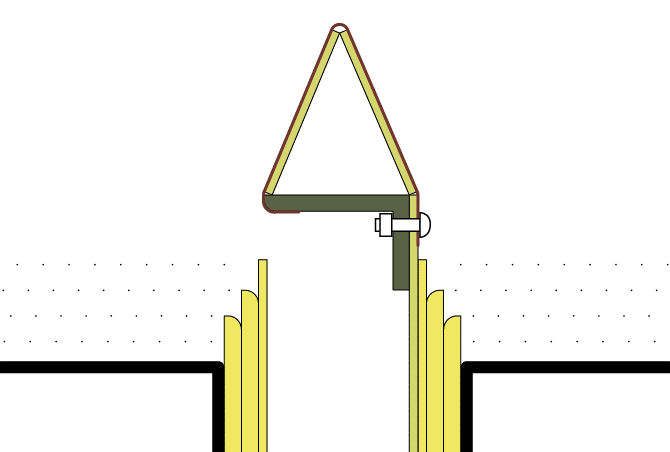
\includegraphics[width=0.55\textwidth]{sp-apa-ed-large.png} 
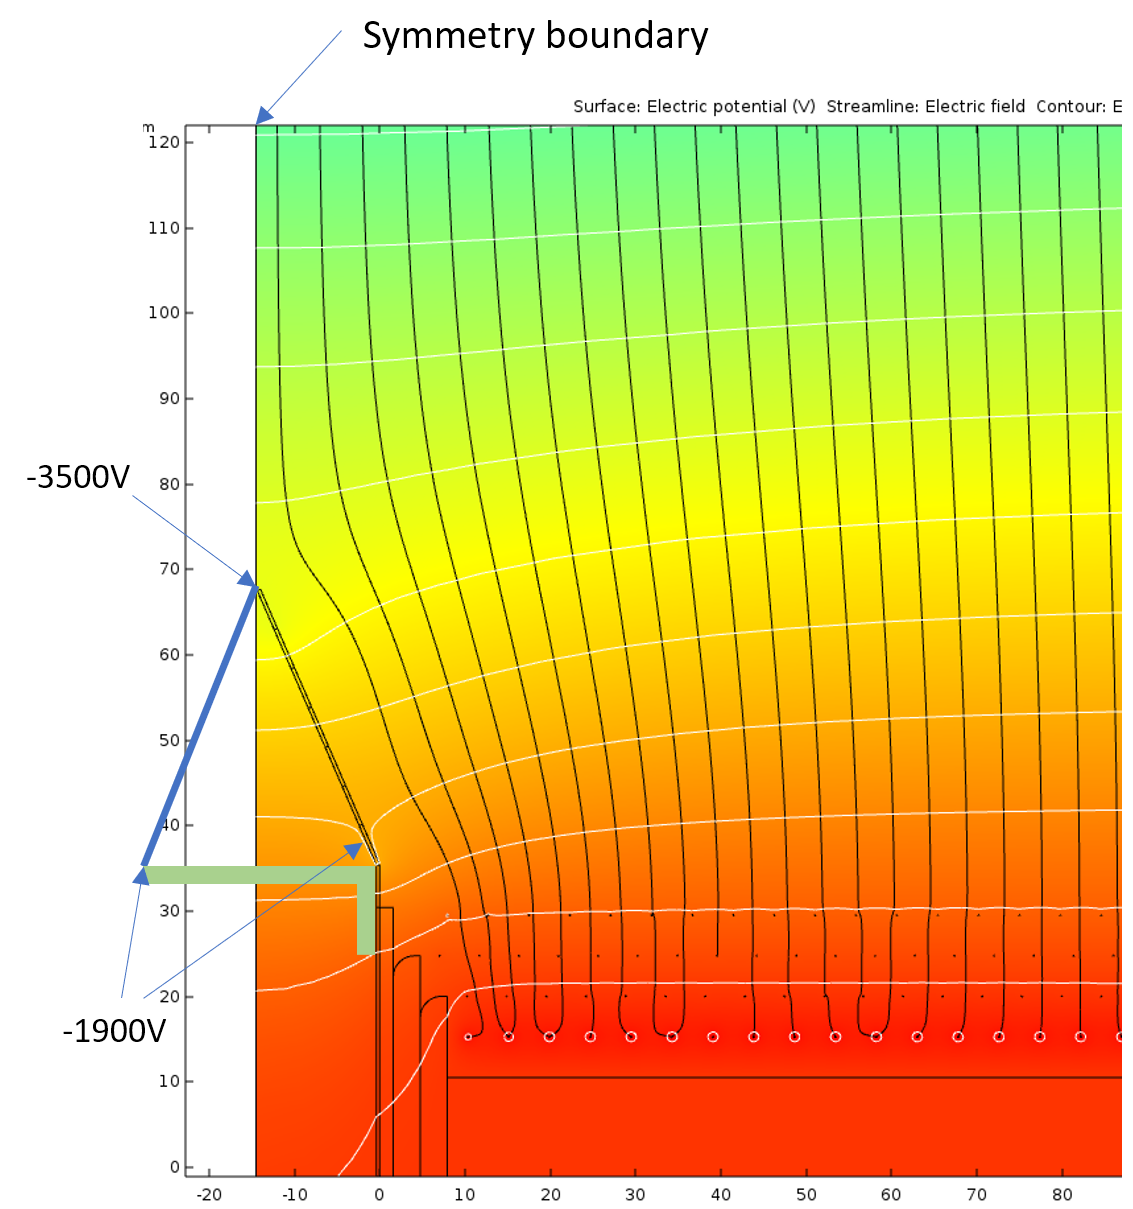
\includegraphics[width=0.4\textwidth]{sp-apa-ed-large-fea.png} 
\end{dunefigure}

\end{comment}


